\documentclass[twoside]{book}

% Packages required by doxygen
\usepackage{fixltx2e}
\usepackage{calc}
\usepackage{doxygen}
\usepackage[export]{adjustbox} % also loads graphicx
\usepackage{graphicx}
\usepackage[utf8]{inputenc}
\usepackage{makeidx}
\usepackage{multicol}
\usepackage{multirow}
\PassOptionsToPackage{warn}{textcomp}
\usepackage{textcomp}
\usepackage[nointegrals]{wasysym}
\usepackage[table]{xcolor}

% Font selection
\usepackage[T1]{fontenc}
\usepackage[scaled=.90]{helvet}
\usepackage{courier}
\usepackage{amssymb}
\usepackage{sectsty}
\renewcommand{\familydefault}{\sfdefault}
\allsectionsfont{%
  \fontseries{bc}\selectfont%
  \color{darkgray}%
}
\renewcommand{\DoxyLabelFont}{%
  \fontseries{bc}\selectfont%
  \color{darkgray}%
}
\newcommand{\+}{\discretionary{\mbox{\scriptsize$\hookleftarrow$}}{}{}}

% Page & text layout
\usepackage{geometry}
\geometry{%
  a4paper,%
  top=2.5cm,%
  bottom=2.5cm,%
  left=2.5cm,%
  right=2.5cm%
}
\tolerance=750
\hfuzz=15pt
\hbadness=750
\setlength{\emergencystretch}{15pt}
\setlength{\parindent}{0cm}
\setlength{\parskip}{3ex plus 2ex minus 2ex}
\makeatletter
\renewcommand{\paragraph}{%
  \@startsection{paragraph}{4}{0ex}{-1.0ex}{1.0ex}{%
    \normalfont\normalsize\bfseries\SS@parafont%
  }%
}
\renewcommand{\subparagraph}{%
  \@startsection{subparagraph}{5}{0ex}{-1.0ex}{1.0ex}{%
    \normalfont\normalsize\bfseries\SS@subparafont%
  }%
}
\makeatother

% Headers & footers
\usepackage{fancyhdr}
\pagestyle{fancyplain}
\fancyhead[LE]{\fancyplain{}{\bfseries\thepage}}
\fancyhead[CE]{\fancyplain{}{}}
\fancyhead[RE]{\fancyplain{}{\bfseries\leftmark}}
\fancyhead[LO]{\fancyplain{}{\bfseries\rightmark}}
\fancyhead[CO]{\fancyplain{}{}}
\fancyhead[RO]{\fancyplain{}{\bfseries\thepage}}
\fancyfoot[LE]{\fancyplain{}{}}
\fancyfoot[CE]{\fancyplain{}{}}
\fancyfoot[RE]{\fancyplain{}{\bfseries\scriptsize Generated by Doxygen }}
\fancyfoot[LO]{\fancyplain{}{\bfseries\scriptsize Generated by Doxygen }}
\fancyfoot[CO]{\fancyplain{}{}}
\fancyfoot[RO]{\fancyplain{}{}}
\renewcommand{\footrulewidth}{0.4pt}
\renewcommand{\chaptermark}[1]{%
  \markboth{#1}{}%
}
\renewcommand{\sectionmark}[1]{%
  \markright{\thesection\ #1}%
}

% Indices & bibliography
\usepackage{natbib}
\usepackage[titles]{tocloft}
\setcounter{tocdepth}{3}
\setcounter{secnumdepth}{5}
\makeindex

% Hyperlinks (required, but should be loaded last)
\usepackage{ifpdf}
\ifpdf
  \usepackage[pdftex,pagebackref=true]{hyperref}
\else
  \usepackage[ps2pdf,pagebackref=true]{hyperref}
\fi
\hypersetup{%
  colorlinks=true,%
  linkcolor=blue,%
  citecolor=blue,%
  unicode%
}

% Custom commands
\newcommand{\clearemptydoublepage}{%
  \newpage{\pagestyle{empty}\cleardoublepage}%
}

\usepackage{caption}
\captionsetup{labelsep=space,justification=centering,font={bf},singlelinecheck=off,skip=4pt,position=top}

%===== C O N T E N T S =====

\begin{document}

% Titlepage & ToC
\hypersetup{pageanchor=false,
             bookmarksnumbered=true,
             pdfencoding=unicode
            }
\pagenumbering{alph}
\begin{titlepage}
\vspace*{7cm}
\begin{center}%
{\Large Zelta\+Lib }\\
\vspace*{1cm}
{\large Generated by Doxygen 1.8.13}\\
\end{center}
\end{titlepage}
\clearemptydoublepage
\pagenumbering{roman}
\tableofcontents
\clearemptydoublepage
\pagenumbering{arabic}
\hypersetup{pageanchor=true}

%--- Begin generated contents ---
\chapter{Hierarchical Index}
\section{Class Hierarchy}
This inheritance list is sorted roughly, but not completely, alphabetically\+:\begin{DoxyCompactList}
\item \contentsline{section}{zt\+:\+:Animatable}{\pageref{classzt_1_1_animatable}}{}
\begin{DoxyCompactList}
\item \contentsline{section}{zt\+:\+:Animatable\+Container}{\pageref{classzt_1_1_animatable_container}}{}
\item \contentsline{section}{zt\+:\+:Scene}{\pageref{classzt_1_1_scene}}{}
\end{DoxyCompactList}
\item \contentsline{section}{zt\+:\+:Application}{\pageref{classzt_1_1_application}}{}
\item \contentsline{section}{zt\+:\+:Argument}{\pageref{classzt_1_1_argument}}{}
\item \contentsline{section}{zt\+:\+:Arguments}{\pageref{classzt_1_1_arguments}}{}
\item \contentsline{section}{zt\+:\+:Auto\+Lang}{\pageref{classzt_1_1_auto_lang}}{}
\item Clock\begin{DoxyCompactList}
\item \contentsline{section}{zt\+:\+:Clock}{\pageref{classzt_1_1_clock}}{}
\begin{DoxyCompactList}
\item \contentsline{section}{zt\+:\+:Nestable\+Clock}{\pageref{classzt_1_1_nestable_clock}}{}
\end{DoxyCompactList}
\end{DoxyCompactList}
\item \contentsline{section}{zt\+:\+:Discovered\+Node$<$ Node\+Type $>$}{\pageref{classzt_1_1_discovered_node}}{}
\item Drawable\begin{DoxyCompactList}
\item \contentsline{section}{zt\+:\+:Render\+Layer}{\pageref{classzt_1_1_render_layer}}{}
\item \contentsline{section}{zt\+:\+:Tilemap\+Layer$<$ T $>$}{\pageref{classzt_1_1_tilemap_layer}}{}
\item \contentsline{section}{zt\+:\+:Tilemap\+Renderer$<$ T $>$}{\pageref{classzt_1_1_tilemap_renderer}}{}
\end{DoxyCompactList}
\item exception\begin{DoxyCompactList}
\item \contentsline{section}{zt\+:\+:File\+Not\+Found\+Exception}{\pageref{classzt_1_1_file_not_found_exception}}{}
\item \contentsline{section}{zt\+:\+:Resource\+Not\+Found\+Exception}{\pageref{classzt_1_1_resource_not_found_exception}}{}
\end{DoxyCompactList}
\item \contentsline{section}{zt\+:\+:I\+Mesh$<$ Node\+Type $>$}{\pageref{classzt_1_1_i_mesh}}{}
\item \contentsline{section}{zt\+:\+:I\+Node}{\pageref{classzt_1_1_i_node}}{}
\item \contentsline{section}{zt\+:\+:tiled\+:\+:Layer}{\pageref{classzt_1_1tiled_1_1_layer}}{}
\item \contentsline{section}{zt\+:\+:Loading\+Target}{\pageref{classzt_1_1_loading_target}}{}
\begin{DoxyCompactList}
\item \contentsline{section}{zt\+:\+:Resource\+Manager$<$ sf\+:\+:Font $>$}{\pageref{classzt_1_1_resource_manager}}{}
\begin{DoxyCompactList}
\item \contentsline{section}{zt\+:\+:Font\+Manager}{\pageref{classzt_1_1_font_manager}}{}
\end{DoxyCompactList}
\item \contentsline{section}{zt\+:\+:Resource\+Manager$<$ sf\+:\+:Sound\+Buffer $>$}{\pageref{classzt_1_1_resource_manager}}{}
\begin{DoxyCompactList}
\item \contentsline{section}{zt\+:\+:Sound\+Buffer\+Manager}{\pageref{classzt_1_1_sound_buffer_manager}}{}
\end{DoxyCompactList}
\item \contentsline{section}{zt\+:\+:Resource\+Manager$<$ sf\+:\+:Texture $>$}{\pageref{classzt_1_1_resource_manager}}{}
\begin{DoxyCompactList}
\item \contentsline{section}{zt\+:\+:Texture\+Manager}{\pageref{classzt_1_1_texture_manager}}{}
\end{DoxyCompactList}
\item \contentsline{section}{zt\+:\+:Resource\+Manager$<$ X $>$}{\pageref{classzt_1_1_resource_manager}}{}
\end{DoxyCompactList}
\item \contentsline{section}{zt\+:\+:Log}{\pageref{classzt_1_1_log}}{}
\begin{DoxyCompactList}
\item \contentsline{section}{zt\+:\+:Console\+Log}{\pageref{classzt_1_1_console_log}}{}
\item \contentsline{section}{zt\+:\+:File\+Log}{\pageref{classzt_1_1_file_log}}{}
\end{DoxyCompactList}
\item \contentsline{section}{zt\+:\+:tiled\+:\+:Map}{\pageref{classzt_1_1tiled_1_1_map}}{}
\item \contentsline{section}{zt\+:\+:tiled\+:\+:Object}{\pageref{classzt_1_1tiled_1_1_object}}{}
\item \contentsline{section}{zt\+:\+:tiled\+:\+:Object\+Layer}{\pageref{classzt_1_1tiled_1_1_object_layer}}{}
\item \contentsline{section}{zt\+:\+:Package}{\pageref{classzt_1_1_package}}{}
\item \contentsline{section}{zt\+:\+:Package\+File\+Info}{\pageref{classzt_1_1_package_file_info}}{}
\item \contentsline{section}{zt\+:\+:Pathfinding$<$ Node\+Type $>$}{\pageref{classzt_1_1_pathfinding}}{}
\item \contentsline{section}{zt\+:\+:Resource\+Provider}{\pageref{classzt_1_1_resource_provider}}{}
\item \contentsline{section}{zt\+:\+:Scene\+Manager}{\pageref{classzt_1_1_scene_manager}}{}
\item \contentsline{section}{zt\+:\+:Screen\+Dimensions}{\pageref{classzt_1_1_screen_dimensions}}{}
\item \contentsline{section}{zt\+:\+:Singleton$<$ T $>$}{\pageref{classzt_1_1_singleton}}{}
\item \contentsline{section}{zt\+:\+:Task}{\pageref{classzt_1_1_task}}{}
\item \contentsline{section}{zt\+:\+:Task\+Pool}{\pageref{classzt_1_1_task_pool}}{}
\item Text\begin{DoxyCompactList}
\item \contentsline{section}{zt\+:\+:Text}{\pageref{classzt_1_1_text}}{}
\end{DoxyCompactList}
\item \contentsline{section}{zt\+:\+:Text\+Container}{\pageref{classzt_1_1_text_container}}{}
\item \contentsline{section}{zt\+:\+:tiled\+:\+:Tile}{\pageref{classzt_1_1tiled_1_1_tile}}{}
\item \contentsline{section}{zt\+:\+:Tile\+Container$<$ T $>$}{\pageref{classzt_1_1_tile_container}}{}
\item \contentsline{section}{zt\+:\+:tiled\+:\+:Tiled\+Loader}{\pageref{classzt_1_1tiled_1_1_tiled_loader}}{}
\item \contentsline{section}{zt\+:\+:Tileset}{\pageref{classzt_1_1_tileset}}{}
\item \contentsline{section}{zt\+:\+:Vector2f}{\pageref{classzt_1_1_vector2f}}{}
\item \contentsline{section}{zt\+:\+:Vector3f}{\pageref{classzt_1_1_vector3f}}{}
\item \contentsline{section}{zt\+:\+:Worker}{\pageref{classzt_1_1_worker}}{}
\end{DoxyCompactList}

\chapter{Class Index}
\section{Class List}
Here are the classes, structs, unions and interfaces with brief descriptions\+:\begin{DoxyCompactList}
\item\contentsline{section}{\hyperlink{classzt_1_1_animatable}{zt\+::\+Animatable} \\*\hyperlink{classzt_1_1_animatable}{Animatable} is a interface used to represent something that changes over time (that\textquotesingle{}s the reason its advance\+Time() method takes the delta time as parameter) }{\pageref{classzt_1_1_animatable}}{}
\item\contentsline{section}{\hyperlink{classzt_1_1_animatable_container}{zt\+::\+Animatable\+Container} \\*Container of \hyperlink{classzt_1_1_animatable}{Animatable} objects }{\pageref{classzt_1_1_animatable_container}}{}
\item\contentsline{section}{\hyperlink{classzt_1_1_application}{zt\+::\+Application} \\*This class is the main class of your program. Generally, this will be the first class to be instantiated and the last one to be destroyed. It does nothing special }{\pageref{classzt_1_1_application}}{}
\item\contentsline{section}{\hyperlink{classzt_1_1_argument}{zt\+::\+Argument} \\*Represents an argument }{\pageref{classzt_1_1_argument}}{}
\item\contentsline{section}{\hyperlink{classzt_1_1_arguments}{zt\+::\+Arguments} \\*Represents a set of arguments (e.\+g.\+: the command line arguments) }{\pageref{classzt_1_1_arguments}}{}
\item\contentsline{section}{\hyperlink{classzt_1_1_clock}{zt\+::\+Clock} \\*Class that measures time. Unlike sf\+::\+Clock, this one can be paused }{\pageref{classzt_1_1_clock}}{}
\item\contentsline{section}{\hyperlink{classzt_1_1_console_log}{zt\+::\+Console\+Log} \\*Class for logging to the console }{\pageref{classzt_1_1_console_log}}{}
\item\contentsline{section}{\hyperlink{classzt_1_1_discovered_node}{zt\+::\+Discovered\+Node$<$ Node\+Type $>$} }{\pageref{classzt_1_1_discovered_node}}{}
\item\contentsline{section}{\hyperlink{classzt_1_1_file_log}{zt\+::\+File\+Log} \\*Class for logging to a file }{\pageref{classzt_1_1_file_log}}{}
\item\contentsline{section}{\hyperlink{classzt_1_1_file_not_found_exception}{zt\+::\+File\+Not\+Found\+Exception} \\*Exception throwed when a file is not found }{\pageref{classzt_1_1_file_not_found_exception}}{}
\item\contentsline{section}{\hyperlink{classzt_1_1_font_manager}{zt\+::\+Font\+Manager} \\*Resource manager for sf\+::\+Font }{\pageref{classzt_1_1_font_manager}}{}
\item\contentsline{section}{\hyperlink{classzt_1_1_i_mesh}{zt\+::\+I\+Mesh$<$ Node\+Type $>$} }{\pageref{classzt_1_1_i_mesh}}{}
\item\contentsline{section}{\hyperlink{classzt_1_1_i_node}{zt\+::\+I\+Node} }{\pageref{classzt_1_1_i_node}}{}
\item\contentsline{section}{\hyperlink{classzt_1_1tiled_1_1_layer}{zt\+::tiled\+::\+Layer} }{\pageref{classzt_1_1tiled_1_1_layer}}{}
\item\contentsline{section}{\hyperlink{classzt_1_1_loading_target}{zt\+::\+Loading\+Target} \\*Base class for resource containers. It represents something you can load things into }{\pageref{classzt_1_1_loading_target}}{}
\item\contentsline{section}{\hyperlink{classzt_1_1_log}{zt\+::\+Log} \\*Base class for logging }{\pageref{classzt_1_1_log}}{}
\item\contentsline{section}{\hyperlink{classzt_1_1tiled_1_1_map}{zt\+::tiled\+::\+Map} }{\pageref{classzt_1_1tiled_1_1_map}}{}
\item\contentsline{section}{\hyperlink{classzt_1_1_nestable_clock}{zt\+::\+Nestable\+Clock} }{\pageref{classzt_1_1_nestable_clock}}{}
\item\contentsline{section}{\hyperlink{classzt_1_1tiled_1_1_object}{zt\+::tiled\+::\+Object} }{\pageref{classzt_1_1tiled_1_1_object}}{}
\item\contentsline{section}{\hyperlink{classzt_1_1tiled_1_1_object_layer}{zt\+::tiled\+::\+Object\+Layer} }{\pageref{classzt_1_1tiled_1_1_object_layer}}{}
\item\contentsline{section}{\hyperlink{classzt_1_1_package}{zt\+::\+Package} \\*Allows you to store all your assets (images, sounds, fonts) in the same file. The class also lets you load those files from the package easily }{\pageref{classzt_1_1_package}}{}
\item\contentsline{section}{\hyperlink{classzt_1_1_package_file_info}{zt\+::\+Package\+File\+Info} }{\pageref{classzt_1_1_package_file_info}}{}
\item\contentsline{section}{\hyperlink{classzt_1_1_pathfinding}{zt\+::\+Pathfinding$<$ Node\+Type $>$} \\*A$\ast$ algorithm implementation }{\pageref{classzt_1_1_pathfinding}}{}
\item\contentsline{section}{\hyperlink{classzt_1_1_render_layer}{zt\+::\+Render\+Layer} \\*Container for drawable objects. This class allows you to group sf\+::\+Drawable elements such as sf\+::\+Sprite. The container keeps pointers to the objects, so your drawable objects should be kept alive while using the render layer }{\pageref{classzt_1_1_render_layer}}{}
\item\contentsline{section}{\hyperlink{classzt_1_1_resource_manager}{zt\+::\+Resource\+Manager$<$ X $>$} \\*Base class for resource managers. A resource manager acts as a container for a specific resource type (e.\+g.\+: a sf\+::\+Texture, sf\+::\+Sound\+Buffer) }{\pageref{classzt_1_1_resource_manager}}{}
\item\contentsline{section}{\hyperlink{classzt_1_1_resource_not_found_exception}{zt\+::\+Resource\+Not\+Found\+Exception} \\*Exception throwed when a resource is not found }{\pageref{classzt_1_1_resource_not_found_exception}}{}
\item\contentsline{section}{\hyperlink{classzt_1_1_resource_provider}{zt\+::\+Resource\+Provider} \\*This class allows you to load resources from the filesystem or a package }{\pageref{classzt_1_1_resource_provider}}{}
\item\contentsline{section}{\hyperlink{classzt_1_1_scene}{zt\+::\+Scene} \\*Represents a game scene. It could be the main menu, the credits scene, etc. This class is made to be inherited from it. Scenes must have a unique name }{\pageref{classzt_1_1_scene}}{}
\item\contentsline{section}{\hyperlink{classzt_1_1_scene_manager}{zt\+::\+Scene\+Manager} \\*This class manages scenes. Scenes added to the scene manager must have a unique name. You\textquotesingle{}ll activate them through the \hyperlink{classzt_1_1_scene_manager}{Scene\+Manager} }{\pageref{classzt_1_1_scene_manager}}{}
\item\contentsline{section}{\hyperlink{classzt_1_1_screen_dimensions}{zt\+::\+Screen\+Dimensions} \\*This class performs some calculations to keep aspect ratio }{\pageref{classzt_1_1_screen_dimensions}}{}
\item\contentsline{section}{\hyperlink{classzt_1_1_singleton}{zt\+::\+Singleton$<$ T $>$} \\*Base class for other singleton classes }{\pageref{classzt_1_1_singleton}}{}
\item\contentsline{section}{\hyperlink{classzt_1_1_sound_buffer_manager}{zt\+::\+Sound\+Buffer\+Manager} \\*Resource manager for sf\+::\+Sound\+Buffer }{\pageref{classzt_1_1_sound_buffer_manager}}{}
\item\contentsline{section}{\hyperlink{classzt_1_1_task}{zt\+::\+Task} \\*A \hyperlink{classzt_1_1_task}{Task} is a unit of work }{\pageref{classzt_1_1_task}}{}
\item\contentsline{section}{\hyperlink{classzt_1_1_task_pool}{zt\+::\+Task\+Pool} \\*A \hyperlink{classzt_1_1_task_pool}{Task\+Pool} keeps a set of workers (threads represented by the \hyperlink{classzt_1_1_worker}{Worker} class). You can enqueue tasks in the \hyperlink{classzt_1_1_task_pool}{Task\+Pool} and they will be executed when a worker is free }{\pageref{classzt_1_1_task_pool}}{}
\item\contentsline{section}{\hyperlink{classzt_1_1_text}{zt\+::\+Text} }{\pageref{classzt_1_1_text}}{}
\item\contentsline{section}{\hyperlink{classzt_1_1_texture_manager}{zt\+::\+Texture\+Manager} \\*Resource manager for sf\+::\+Texture }{\pageref{classzt_1_1_texture_manager}}{}
\item\contentsline{section}{\hyperlink{classzt_1_1tiled_1_1_tile}{zt\+::tiled\+::\+Tile} }{\pageref{classzt_1_1tiled_1_1_tile}}{}
\item\contentsline{section}{\hyperlink{classzt_1_1_tile_container}{zt\+::\+Tile\+Container$<$ T $>$} }{\pageref{classzt_1_1_tile_container}}{}
\item\contentsline{section}{\hyperlink{classzt_1_1tiled_1_1_tiled_loader}{zt\+::tiled\+::\+Tiled\+Loader} }{\pageref{classzt_1_1tiled_1_1_tiled_loader}}{}
\item\contentsline{section}{\hyperlink{classzt_1_1_tilemap_layer}{zt\+::\+Tilemap\+Layer$<$ T $>$} }{\pageref{classzt_1_1_tilemap_layer}}{}
\item\contentsline{section}{\hyperlink{classzt_1_1_tilemap_renderer}{zt\+::\+Tilemap\+Renderer$<$ T $>$} }{\pageref{classzt_1_1_tilemap_renderer}}{}
\item\contentsline{section}{\hyperlink{classzt_1_1_tileset}{zt\+::\+Tileset} }{\pageref{classzt_1_1_tileset}}{}
\item\contentsline{section}{\hyperlink{classzt_1_1_vector2f}{zt\+::\+Vector2f} \\*Utility class for 2-\/dimensional vectors }{\pageref{classzt_1_1_vector2f}}{}
\item\contentsline{section}{\hyperlink{classzt_1_1_vector3f}{zt\+::\+Vector3f} \\*Utility class for 3-\/dimensional vectors }{\pageref{classzt_1_1_vector3f}}{}
\item\contentsline{section}{\hyperlink{classzt_1_1_worker}{zt\+::\+Worker} \\*Represents a thread. A \hyperlink{classzt_1_1_worker}{Worker} can have one task assigned at a time. It communicates with the \hyperlink{classzt_1_1_task_pool}{Task\+Pool} through a condition\+\_\+variable to send notifications when the task is done }{\pageref{classzt_1_1_worker}}{}
\end{DoxyCompactList}

\chapter{Class Documentation}
\hypertarget{classzt_1_1_animatable}{}\section{zt\+:\+:Animatable Class Reference}
\label{classzt_1_1_animatable}\index{zt\+::\+Animatable@{zt\+::\+Animatable}}


\hyperlink{classzt_1_1_animatable}{Animatable} is a interface used to represent something that changes over time (that\textquotesingle{}s the reason its advance\+Time() method takes the delta time as parameter).  




{\ttfamily \#include $<$Animatable.\+hpp$>$}

Inheritance diagram for zt\+:\+:Animatable\+:\begin{figure}[H]
\begin{center}
\leavevmode
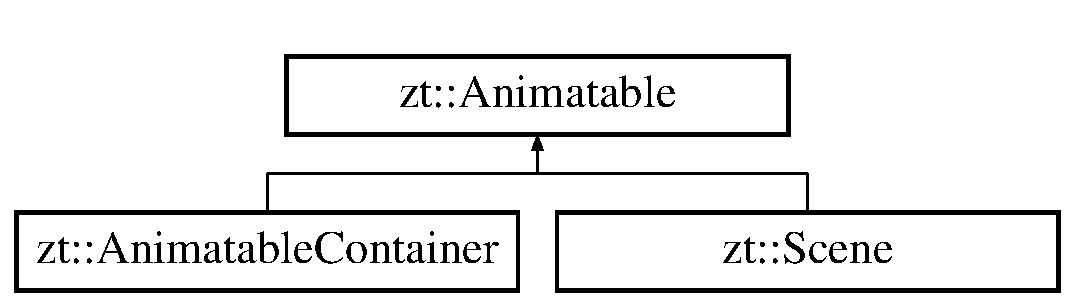
\includegraphics[height=2.000000cm]{classzt_1_1_animatable}
\end{center}
\end{figure}
\subsection*{Public Member Functions}
\begin{DoxyCompactItemize}
\item 
\mbox{\Hypertarget{classzt_1_1_animatable_a9d411c0fb6df48f5d6e5c6f72ee1019e}\label{classzt_1_1_animatable_a9d411c0fb6df48f5d6e5c6f72ee1019e}} 
virtual void {\bfseries advance\+Time} (float delta\+Time)=0
\end{DoxyCompactItemize}


\subsection{Detailed Description}
\hyperlink{classzt_1_1_animatable}{Animatable} is a interface used to represent something that changes over time (that\textquotesingle{}s the reason its advance\+Time() method takes the delta time as parameter). 

The documentation for this class was generated from the following file\+:\begin{DoxyCompactItemize}
\item 
include/\+Zelta/\+Core/Animatable.\+hpp\end{DoxyCompactItemize}

\hypertarget{classzt_1_1_animatable_container}{}\section{zt\+:\+:Animatable\+Container Class Reference}
\label{classzt_1_1_animatable_container}\index{zt\+::\+Animatable\+Container@{zt\+::\+Animatable\+Container}}


Container of \hyperlink{classzt_1_1_animatable}{Animatable} objects.  




{\ttfamily \#include $<$Animatable\+Container.\+hpp$>$}

Inheritance diagram for zt\+:\+:Animatable\+Container\+:\begin{figure}[H]
\begin{center}
\leavevmode
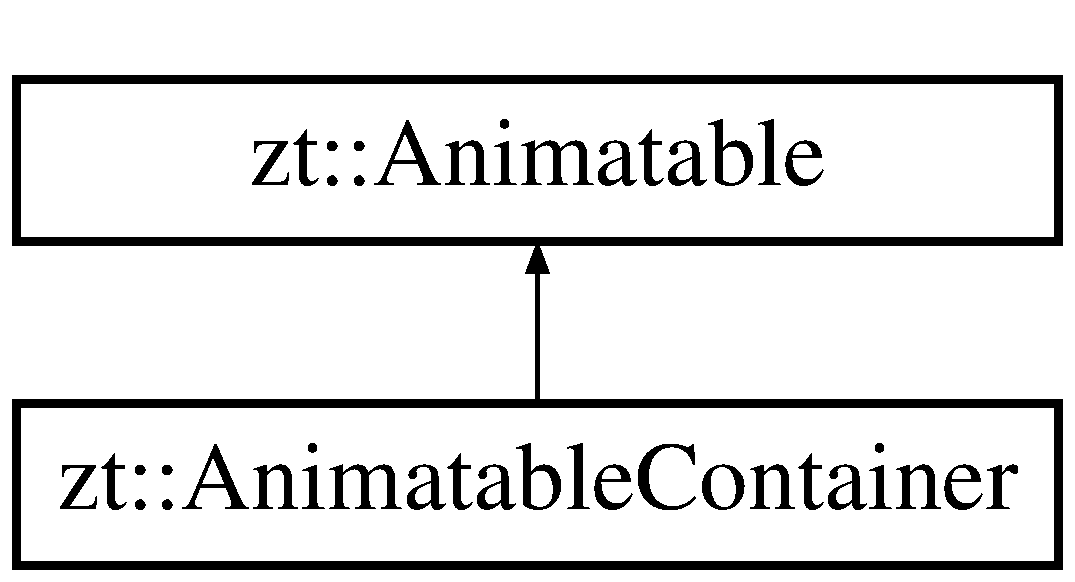
\includegraphics[height=2.000000cm]{classzt_1_1_animatable_container}
\end{center}
\end{figure}
\subsection*{Public Member Functions}
\begin{DoxyCompactItemize}
\item 
void \hyperlink{classzt_1_1_animatable_container_a4288e8efa0335f0f34b678a9f5b92219}{add} (\hyperlink{classzt_1_1_animatable}{Animatable} \&animatable)
\begin{DoxyCompactList}\small\item\em Adds an \hyperlink{classzt_1_1_animatable}{Animatable} to the container. \end{DoxyCompactList}\item 
void \hyperlink{classzt_1_1_animatable_container_ac6086455938dd4285bd6f7beca7d2eeb}{remove} (\hyperlink{classzt_1_1_animatable}{Animatable} \&animatable)
\begin{DoxyCompactList}\small\item\em Removes an \hyperlink{classzt_1_1_animatable}{Animatable} from the container. \end{DoxyCompactList}\item 
\mbox{\Hypertarget{classzt_1_1_animatable_container_a51c0d2047544bb0bc49162a5c8a303ce}\label{classzt_1_1_animatable_container_a51c0d2047544bb0bc49162a5c8a303ce}} 
void {\bfseries advance\+Time} (float delta\+Time)
\item 
bool \hyperlink{classzt_1_1_animatable_container_ad9101ffe27f3615e72bc66b04061b737}{is\+Paused} () const
\item 
void \hyperlink{classzt_1_1_animatable_container_a7c05633b4d68f39617f8ccc9bd752beb}{pause} ()
\begin{DoxyCompactList}\small\item\em Pauses all child animatable objects. \end{DoxyCompactList}\item 
\mbox{\Hypertarget{classzt_1_1_animatable_container_a82fbd2812fbcfeaae56397730ae6468b}\label{classzt_1_1_animatable_container_a82fbd2812fbcfeaae56397730ae6468b}} 
void \hyperlink{classzt_1_1_animatable_container_a82fbd2812fbcfeaae56397730ae6468b}{resume} ()
\begin{DoxyCompactList}\small\item\em Resumes all child animatable objects. \end{DoxyCompactList}\end{DoxyCompactItemize}


\subsection{Detailed Description}
Container of \hyperlink{classzt_1_1_animatable}{Animatable} objects. 

\subsection{Member Function Documentation}
\mbox{\Hypertarget{classzt_1_1_animatable_container_a4288e8efa0335f0f34b678a9f5b92219}\label{classzt_1_1_animatable_container_a4288e8efa0335f0f34b678a9f5b92219}} 
\index{zt\+::\+Animatable\+Container@{zt\+::\+Animatable\+Container}!add@{add}}
\index{add@{add}!zt\+::\+Animatable\+Container@{zt\+::\+Animatable\+Container}}
\subsubsection{\texorpdfstring{add()}{add()}}
{\footnotesize\ttfamily void zt\+::\+Animatable\+Container\+::add (\begin{DoxyParamCaption}\item[{\hyperlink{classzt_1_1_animatable}{Animatable} \&}]{animatable }\end{DoxyParamCaption})}



Adds an \hyperlink{classzt_1_1_animatable}{Animatable} to the container. 


\begin{DoxyParams}{Parameters}
{\em animatable} & \hyperlink{classzt_1_1_animatable}{Animatable}. \\
\hline
\end{DoxyParams}
\mbox{\Hypertarget{classzt_1_1_animatable_container_ad9101ffe27f3615e72bc66b04061b737}\label{classzt_1_1_animatable_container_ad9101ffe27f3615e72bc66b04061b737}} 
\index{zt\+::\+Animatable\+Container@{zt\+::\+Animatable\+Container}!is\+Paused@{is\+Paused}}
\index{is\+Paused@{is\+Paused}!zt\+::\+Animatable\+Container@{zt\+::\+Animatable\+Container}}
\subsubsection{\texorpdfstring{is\+Paused()}{isPaused()}}
{\footnotesize\ttfamily bool zt\+::\+Animatable\+Container\+::is\+Paused (\begin{DoxyParamCaption}{ }\end{DoxyParamCaption}) const}

\begin{DoxyReturn}{Returns}
Devuelve true si está pausado. 
\end{DoxyReturn}
\mbox{\Hypertarget{classzt_1_1_animatable_container_a7c05633b4d68f39617f8ccc9bd752beb}\label{classzt_1_1_animatable_container_a7c05633b4d68f39617f8ccc9bd752beb}} 
\index{zt\+::\+Animatable\+Container@{zt\+::\+Animatable\+Container}!pause@{pause}}
\index{pause@{pause}!zt\+::\+Animatable\+Container@{zt\+::\+Animatable\+Container}}
\subsubsection{\texorpdfstring{pause()}{pause()}}
{\footnotesize\ttfamily void zt\+::\+Animatable\+Container\+::pause (\begin{DoxyParamCaption}{ }\end{DoxyParamCaption})}



Pauses all child animatable objects. 

When the container is paused, advance\+Time() of child objects are not called. \mbox{\Hypertarget{classzt_1_1_animatable_container_ac6086455938dd4285bd6f7beca7d2eeb}\label{classzt_1_1_animatable_container_ac6086455938dd4285bd6f7beca7d2eeb}} 
\index{zt\+::\+Animatable\+Container@{zt\+::\+Animatable\+Container}!remove@{remove}}
\index{remove@{remove}!zt\+::\+Animatable\+Container@{zt\+::\+Animatable\+Container}}
\subsubsection{\texorpdfstring{remove()}{remove()}}
{\footnotesize\ttfamily void zt\+::\+Animatable\+Container\+::remove (\begin{DoxyParamCaption}\item[{\hyperlink{classzt_1_1_animatable}{Animatable} \&}]{animatable }\end{DoxyParamCaption})}



Removes an \hyperlink{classzt_1_1_animatable}{Animatable} from the container. 


\begin{DoxyParams}{Parameters}
{\em animatable} & \hyperlink{classzt_1_1_animatable}{Animatable}. \\
\hline
\end{DoxyParams}


The documentation for this class was generated from the following file\+:\begin{DoxyCompactItemize}
\item 
include/\+Zelta/\+Core/Animatable\+Container.\+hpp\end{DoxyCompactItemize}

\hypertarget{classzt_1_1_application}{}\section{zt\+:\+:Application Class Reference}
\label{classzt_1_1_application}\index{zt\+::\+Application@{zt\+::\+Application}}


This class is the main class of your program. Generally, this will be the first class to be instantiated and the last one to be destroyed. It does nothing special.  




{\ttfamily \#include $<$Application.\+hpp$>$}

\subsection*{Public Member Functions}
\begin{DoxyCompactItemize}
\item 
\mbox{\Hypertarget{classzt_1_1_application_afa0cd6ed2803717f73d602863f669c40}\label{classzt_1_1_application_afa0cd6ed2803717f73d602863f669c40}} 
{\bfseries Application} (int argc, char $\ast$$\ast$argv)
\item 
\mbox{\Hypertarget{classzt_1_1_application_a90a277ed91c864c953c1c20843b765af}\label{classzt_1_1_application_a90a277ed91c864c953c1c20843b765af}} 
virtual int {\bfseries run} ()=0
\item 
\mbox{\Hypertarget{classzt_1_1_application_a8c1357f7819e739d8c7e88712eab18da}\label{classzt_1_1_application_a8c1357f7819e739d8c7e88712eab18da}} 
virtual const \hyperlink{classzt_1_1_arguments}{Arguments} \& {\bfseries get\+Arguments} () const
\end{DoxyCompactItemize}
\subsection*{Protected Attributes}
\begin{DoxyCompactItemize}
\item 
\mbox{\Hypertarget{classzt_1_1_application_a0ccbf0d4c1aec8b3bc99430e948a8f5b}\label{classzt_1_1_application_a0ccbf0d4c1aec8b3bc99430e948a8f5b}} 
\hyperlink{classzt_1_1_arguments}{Arguments} {\bfseries arguments}
\end{DoxyCompactItemize}


\subsection{Detailed Description}
This class is the main class of your program. Generally, this will be the first class to be instantiated and the last one to be destroyed. It does nothing special. 

The documentation for this class was generated from the following file\+:\begin{DoxyCompactItemize}
\item 
include/\+Zelta/\+Core/Application.\+hpp\end{DoxyCompactItemize}

\hypertarget{classzt_1_1_argument}{}\section{zt\+:\+:Argument Class Reference}
\label{classzt_1_1_argument}\index{zt\+::\+Argument@{zt\+::\+Argument}}


Represents an argument.  




{\ttfamily \#include $<$Argument.\+hpp$>$}

\subsection*{Public Member Functions}
\begin{DoxyCompactItemize}
\item 
\mbox{\Hypertarget{classzt_1_1_argument_ac257d125029defd69739a2caac476238}\label{classzt_1_1_argument_ac257d125029defd69739a2caac476238}} 
{\bfseries Argument} (const std\+::string \&argument)
\item 
\mbox{\Hypertarget{classzt_1_1_argument_af5927508c283ada9b42ca1a077dc0615}\label{classzt_1_1_argument_af5927508c283ada9b42ca1a077dc0615}} 
const std\+::string \& {\bfseries to\+String} () const
\item 
\mbox{\Hypertarget{classzt_1_1_argument_acfa50891baa70815c227bb0f385dcb1c}\label{classzt_1_1_argument_acfa50891baa70815c227bb0f385dcb1c}} 
int {\bfseries to\+Int} () const
\item 
\mbox{\Hypertarget{classzt_1_1_argument_af937ac1ddbfd477a64e1052cbd37e8b7}\label{classzt_1_1_argument_af937ac1ddbfd477a64e1052cbd37e8b7}} 
float {\bfseries to\+Float} () const
\item 
\mbox{\Hypertarget{classzt_1_1_argument_a6242b3657c5a73d3d44cfe7f77488118}\label{classzt_1_1_argument_a6242b3657c5a73d3d44cfe7f77488118}} 
double {\bfseries to\+Double} () const
\end{DoxyCompactItemize}


\subsection{Detailed Description}
Represents an argument. 

The documentation for this class was generated from the following file\+:\begin{DoxyCompactItemize}
\item 
include/\+Zelta/\+Core/Argument.\+hpp\end{DoxyCompactItemize}

\hypertarget{classzt_1_1_arguments}{}\section{zt\+:\+:Arguments Class Reference}
\label{classzt_1_1_arguments}\index{zt\+::\+Arguments@{zt\+::\+Arguments}}


Represents a set of arguments (e.\+g.\+: the command line arguments).  




{\ttfamily \#include $<$Arguments.\+hpp$>$}

\subsection*{Public Member Functions}
\begin{DoxyCompactItemize}
\item 
\mbox{\Hypertarget{classzt_1_1_arguments_a54f00e2e61fa29ba5c371bb858b572aa}\label{classzt_1_1_arguments_a54f00e2e61fa29ba5c371bb858b572aa}} 
\hyperlink{classzt_1_1_arguments_a54f00e2e61fa29ba5c371bb858b572aa}{Arguments} ()
\begin{DoxyCompactList}\small\item\em Crea un conjunto de parámetros vacío. \end{DoxyCompactList}\item 
\hyperlink{classzt_1_1_arguments_a808eb391686c72c4196f4cf59610f427}{Arguments} (int argc, char $\ast$$\ast$argv)
\begin{DoxyCompactList}\small\item\em Conjunto de parámetros a partir de un puntero de punteros. \end{DoxyCompactList}\item 
\mbox{\Hypertarget{classzt_1_1_arguments_a82a314122a0b4944d824fb73bd6242a0}\label{classzt_1_1_arguments_a82a314122a0b4944d824fb73bd6242a0}} 
virtual void {\bfseries initialize} (int argc, char $\ast$$\ast$argv)
\item 
int \hyperlink{classzt_1_1_arguments_aee2e1c74257bd3a11d34edb1898341dc}{size} () const
\item 
const \hyperlink{classzt_1_1_argument}{Argument} \& \hyperlink{classzt_1_1_arguments_a0b71f588f3af4e114149773af8f31c2e}{get} (int i) const
\end{DoxyCompactItemize}


\subsection{Detailed Description}
Represents a set of arguments (e.\+g.\+: the command line arguments). 

\subsection{Constructor \& Destructor Documentation}
\mbox{\Hypertarget{classzt_1_1_arguments_a808eb391686c72c4196f4cf59610f427}\label{classzt_1_1_arguments_a808eb391686c72c4196f4cf59610f427}} 
\index{zt\+::\+Arguments@{zt\+::\+Arguments}!Arguments@{Arguments}}
\index{Arguments@{Arguments}!zt\+::\+Arguments@{zt\+::\+Arguments}}
\subsubsection{\texorpdfstring{Arguments()}{Arguments()}}
{\footnotesize\ttfamily zt\+::\+Arguments\+::\+Arguments (\begin{DoxyParamCaption}\item[{int}]{argc,  }\item[{char $\ast$$\ast$}]{argv }\end{DoxyParamCaption})}



Conjunto de parámetros a partir de un puntero de punteros. 


\begin{DoxyParams}{Parameters}
{\em argc} & Número de parámetros. \\
\hline
{\em argv} & Puntero a cadenas de caracteres. \\
\hline
\end{DoxyParams}


\subsection{Member Function Documentation}
\mbox{\Hypertarget{classzt_1_1_arguments_a0b71f588f3af4e114149773af8f31c2e}\label{classzt_1_1_arguments_a0b71f588f3af4e114149773af8f31c2e}} 
\index{zt\+::\+Arguments@{zt\+::\+Arguments}!get@{get}}
\index{get@{get}!zt\+::\+Arguments@{zt\+::\+Arguments}}
\subsubsection{\texorpdfstring{get()}{get()}}
{\footnotesize\ttfamily const \hyperlink{classzt_1_1_argument}{Argument}\& zt\+::\+Arguments\+::get (\begin{DoxyParamCaption}\item[{int}]{i }\end{DoxyParamCaption}) const}


\begin{DoxyParams}{Parameters}
{\em i} & Índice del parámetro. El 0 debería ser el nombre del ejecutable. \\
\hline
\end{DoxyParams}
\begin{DoxyReturn}{Returns}
Parámetro. 
\end{DoxyReturn}
\mbox{\Hypertarget{classzt_1_1_arguments_aee2e1c74257bd3a11d34edb1898341dc}\label{classzt_1_1_arguments_aee2e1c74257bd3a11d34edb1898341dc}} 
\index{zt\+::\+Arguments@{zt\+::\+Arguments}!size@{size}}
\index{size@{size}!zt\+::\+Arguments@{zt\+::\+Arguments}}
\subsubsection{\texorpdfstring{size()}{size()}}
{\footnotesize\ttfamily int zt\+::\+Arguments\+::size (\begin{DoxyParamCaption}{ }\end{DoxyParamCaption}) const}

\begin{DoxyReturn}{Returns}
Número de parámetros. 
\end{DoxyReturn}


The documentation for this class was generated from the following file\+:\begin{DoxyCompactItemize}
\item 
include/\+Zelta/\+Core/Arguments.\+hpp\end{DoxyCompactItemize}

\hypertarget{classzt_1_1_clock}{}\section{zt\+:\+:Clock Class Reference}
\label{classzt_1_1_clock}\index{zt\+::\+Clock@{zt\+::\+Clock}}


Class that measures time. Unlike sf\+::\+Clock, this one can be paused.  




{\ttfamily \#include $<$Clock.\+hpp$>$}

Inheritance diagram for zt\+:\+:Clock\+:\begin{figure}[H]
\begin{center}
\leavevmode
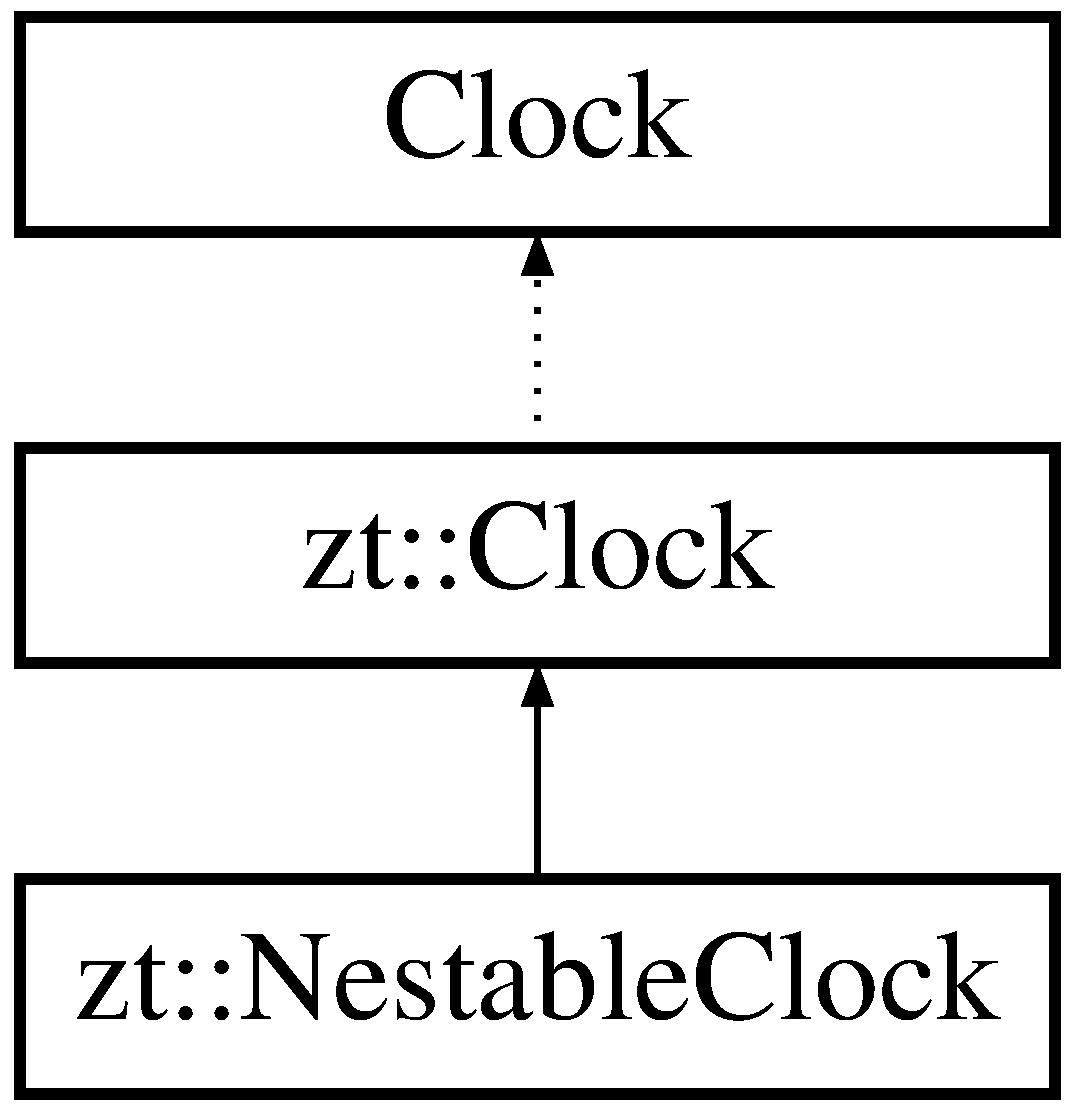
\includegraphics[height=3.000000cm]{classzt_1_1_clock}
\end{center}
\end{figure}
\subsection*{Public Member Functions}
\begin{DoxyCompactItemize}
\item 
sf\+::\+Time \hyperlink{classzt_1_1_clock_a7cd9408d376156ed1ef710ebdeed2615}{get\+Elapsed\+Time} () const
\item 
\mbox{\Hypertarget{classzt_1_1_clock_a58515712a76981f8cbbb4de15ea01198}\label{classzt_1_1_clock_a58515712a76981f8cbbb4de15ea01198}} 
void \hyperlink{classzt_1_1_clock_a58515712a76981f8cbbb4de15ea01198}{pause} ()
\begin{DoxyCompactList}\small\item\em Pauses the clock. \end{DoxyCompactList}\item 
sf\+::\+Time \hyperlink{classzt_1_1_clock_a25742e0b8d93ed9d9a03f1ebc01edd76}{restart} ()
\begin{DoxyCompactList}\small\item\em Restarts the clock. \end{DoxyCompactList}\item 
\mbox{\Hypertarget{classzt_1_1_clock_a5bc290d15ca92741d073e1b96014ad45}\label{classzt_1_1_clock_a5bc290d15ca92741d073e1b96014ad45}} 
void \hyperlink{classzt_1_1_clock_a5bc290d15ca92741d073e1b96014ad45}{resume} ()
\begin{DoxyCompactList}\small\item\em Resumes the clock. \end{DoxyCompactList}\item 
bool \hyperlink{classzt_1_1_clock_ad9ec39488832c24128d8b6af3b20fc80}{is\+Paused} () const
\end{DoxyCompactItemize}


\subsection{Detailed Description}
Class that measures time. Unlike sf\+::\+Clock, this one can be paused. 

\subsection{Member Function Documentation}
\mbox{\Hypertarget{classzt_1_1_clock_a7cd9408d376156ed1ef710ebdeed2615}\label{classzt_1_1_clock_a7cd9408d376156ed1ef710ebdeed2615}} 
\index{zt\+::\+Clock@{zt\+::\+Clock}!get\+Elapsed\+Time@{get\+Elapsed\+Time}}
\index{get\+Elapsed\+Time@{get\+Elapsed\+Time}!zt\+::\+Clock@{zt\+::\+Clock}}
\subsubsection{\texorpdfstring{get\+Elapsed\+Time()}{getElapsedTime()}}
{\footnotesize\ttfamily sf\+::\+Time zt\+::\+Clock\+::get\+Elapsed\+Time (\begin{DoxyParamCaption}{ }\end{DoxyParamCaption}) const}

\begin{DoxyReturn}{Returns}
Returns the elapsed time. 
\end{DoxyReturn}
\mbox{\Hypertarget{classzt_1_1_clock_ad9ec39488832c24128d8b6af3b20fc80}\label{classzt_1_1_clock_ad9ec39488832c24128d8b6af3b20fc80}} 
\index{zt\+::\+Clock@{zt\+::\+Clock}!is\+Paused@{is\+Paused}}
\index{is\+Paused@{is\+Paused}!zt\+::\+Clock@{zt\+::\+Clock}}
\subsubsection{\texorpdfstring{is\+Paused()}{isPaused()}}
{\footnotesize\ttfamily bool zt\+::\+Clock\+::is\+Paused (\begin{DoxyParamCaption}{ }\end{DoxyParamCaption}) const}

\begin{DoxyReturn}{Returns}
True if the clock is paused. 
\end{DoxyReturn}
\mbox{\Hypertarget{classzt_1_1_clock_a25742e0b8d93ed9d9a03f1ebc01edd76}\label{classzt_1_1_clock_a25742e0b8d93ed9d9a03f1ebc01edd76}} 
\index{zt\+::\+Clock@{zt\+::\+Clock}!restart@{restart}}
\index{restart@{restart}!zt\+::\+Clock@{zt\+::\+Clock}}
\subsubsection{\texorpdfstring{restart()}{restart()}}
{\footnotesize\ttfamily sf\+::\+Time zt\+::\+Clock\+::restart (\begin{DoxyParamCaption}{ }\end{DoxyParamCaption})}



Restarts the clock. 

\begin{DoxyReturn}{Returns}
Returns the elapsed time. 
\end{DoxyReturn}


The documentation for this class was generated from the following file\+:\begin{DoxyCompactItemize}
\item 
include/\+Zelta/\+Core/Clock.\+hpp\end{DoxyCompactItemize}

\hypertarget{classzt_1_1_console_log}{}\section{zt\+:\+:Console\+Log Class Reference}
\label{classzt_1_1_console_log}\index{zt\+::\+Console\+Log@{zt\+::\+Console\+Log}}


Class for logging to the console.  




{\ttfamily \#include $<$Console\+Log.\+hpp$>$}

Inheritance diagram for zt\+:\+:Console\+Log\+:\begin{figure}[H]
\begin{center}
\leavevmode
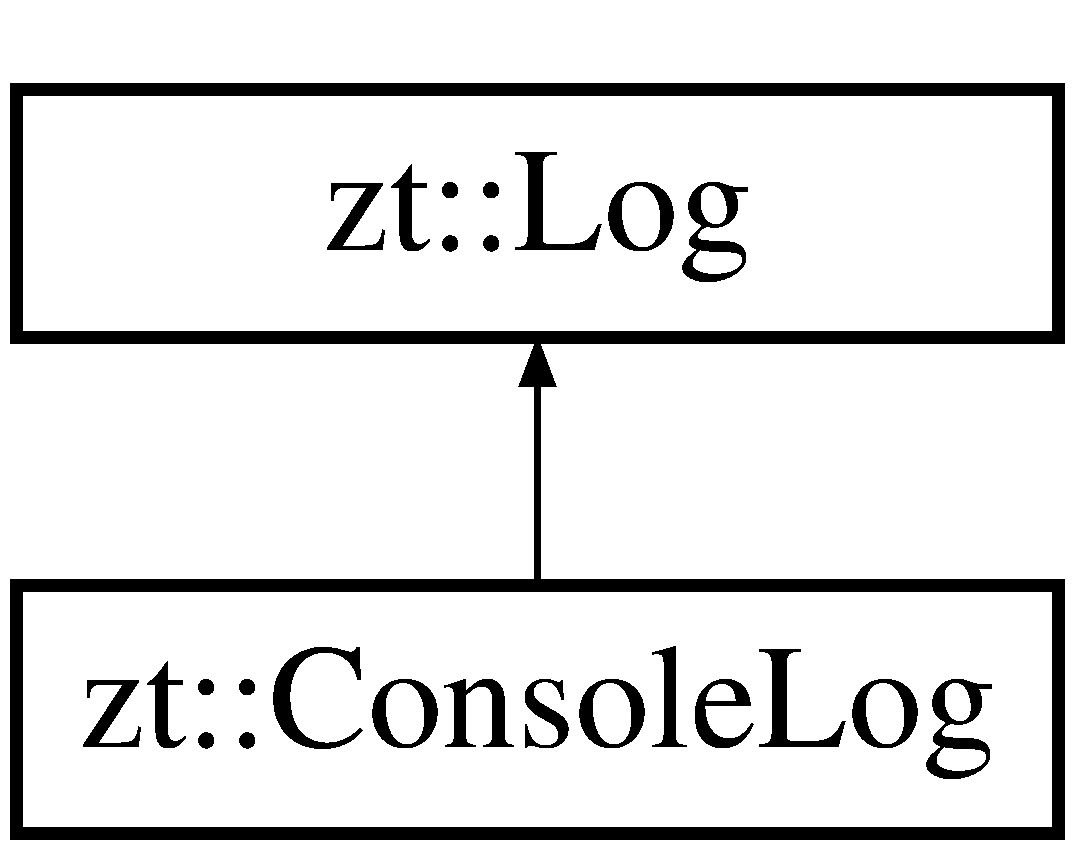
\includegraphics[height=2.000000cm]{classzt_1_1_console_log}
\end{center}
\end{figure}
\subsection*{Public Member Functions}
\begin{DoxyCompactItemize}
\item 
\mbox{\Hypertarget{classzt_1_1_console_log_a79bda0ffa25340ce72ded1cd12d4374b}\label{classzt_1_1_console_log_a79bda0ffa25340ce72ded1cd12d4374b}} 
void {\bfseries log} (Log\+::\+Type type, const std\+::string \&message)
\item 
\mbox{\Hypertarget{classzt_1_1_console_log_a3aa1b87161676976d85aaf34dbd9608d}\label{classzt_1_1_console_log_a3aa1b87161676976d85aaf34dbd9608d}} 
\hyperlink{classzt_1_1_console_log}{Console\+Log} \& {\bfseries operator$<$$<$} (const std\+::string \&message)
\item 
\mbox{\Hypertarget{classzt_1_1_console_log_abae5752feb7fb6bc7ed4c4cf22e04338}\label{classzt_1_1_console_log_abae5752feb7fb6bc7ed4c4cf22e04338}} 
\hyperlink{classzt_1_1_console_log}{Console\+Log} \& {\bfseries operator$<$$<$} (const Log\+::\+Type \&type)
\end{DoxyCompactItemize}
\subsection*{Additional Inherited Members}


\subsection{Detailed Description}
Class for logging to the console. 

The documentation for this class was generated from the following file\+:\begin{DoxyCompactItemize}
\item 
include/\+Zelta/\+Core/Console\+Log.\+hpp\end{DoxyCompactItemize}

\hypertarget{classzt_1_1_discovered_node}{}\section{zt\+:\+:Discovered\+Node$<$ Node\+Type $>$ Class Template Reference}
\label{classzt_1_1_discovered_node}\index{zt\+::\+Discovered\+Node$<$ Node\+Type $>$@{zt\+::\+Discovered\+Node$<$ Node\+Type $>$}}
\subsection*{Public Member Functions}
\begin{DoxyCompactItemize}
\item 
\mbox{\Hypertarget{classzt_1_1_discovered_node_acc9dce4d6f7e699242fb152f5efea7f2}\label{classzt_1_1_discovered_node_acc9dce4d6f7e699242fb152f5efea7f2}} 
{\bfseries Discovered\+Node} (const Node\+Type \&node, float g=0, float h=0)
\item 
\mbox{\Hypertarget{classzt_1_1_discovered_node_a436ccf9eba587d174a4878a6159f6d66}\label{classzt_1_1_discovered_node_a436ccf9eba587d174a4878a6159f6d66}} 
{\bfseries Discovered\+Node} (const Node\+Type \&node, const Node\+Type \&previous\+Node, float g=0, float h=0)
\item 
\mbox{\Hypertarget{classzt_1_1_discovered_node_ac6140ccb435b77f07f46ef586dd2d229}\label{classzt_1_1_discovered_node_ac6140ccb435b77f07f46ef586dd2d229}} 
{\bfseries Discovered\+Node} (const \hyperlink{classzt_1_1_discovered_node}{Discovered\+Node} \&other)
\item 
\mbox{\Hypertarget{classzt_1_1_discovered_node_aeba9dd862ef02be644eb60a0f00c3755}\label{classzt_1_1_discovered_node_aeba9dd862ef02be644eb60a0f00c3755}} 
float {\bfseries f} () const
\item 
\mbox{\Hypertarget{classzt_1_1_discovered_node_a66ffa8ece48f93dc68cdca70b5926b55}\label{classzt_1_1_discovered_node_a66ffa8ece48f93dc68cdca70b5926b55}} 
bool {\bfseries operator==} (const \hyperlink{classzt_1_1_discovered_node}{Discovered\+Node} \&other) const
\end{DoxyCompactItemize}
\subsection*{Public Attributes}
\begin{DoxyCompactItemize}
\item 
\mbox{\Hypertarget{classzt_1_1_discovered_node_abd40a3c5ffa8c7d7eb8acad9947ecfac}\label{classzt_1_1_discovered_node_abd40a3c5ffa8c7d7eb8acad9947ecfac}} 
float {\bfseries g}
\item 
\mbox{\Hypertarget{classzt_1_1_discovered_node_aa7ba76666a021a6241aa50ed14eaf876}\label{classzt_1_1_discovered_node_aa7ba76666a021a6241aa50ed14eaf876}} 
float {\bfseries h}
\item 
\mbox{\Hypertarget{classzt_1_1_discovered_node_a628117da1b7aaa57c668e84ad854cab2}\label{classzt_1_1_discovered_node_a628117da1b7aaa57c668e84ad854cab2}} 
Node\+Type {\bfseries node}
\item 
\mbox{\Hypertarget{classzt_1_1_discovered_node_a360b2f052598bde2eaf7f24a8f9130ce}\label{classzt_1_1_discovered_node_a360b2f052598bde2eaf7f24a8f9130ce}} 
Node\+Type {\bfseries previous\+Node}
\item 
\mbox{\Hypertarget{classzt_1_1_discovered_node_a0c59165132e985ad8cedc2b370cddfe4}\label{classzt_1_1_discovered_node_a0c59165132e985ad8cedc2b370cddfe4}} 
bool {\bfseries initial}
\end{DoxyCompactItemize}


The documentation for this class was generated from the following file\+:\begin{DoxyCompactItemize}
\item 
include/\+Zelta/\+A\+I/Pathfinding.\+hpp\end{DoxyCompactItemize}

\hypertarget{classzt_1_1_file_log}{}\section{zt\+:\+:File\+Log Class Reference}
\label{classzt_1_1_file_log}\index{zt\+::\+File\+Log@{zt\+::\+File\+Log}}


Class for logging to a file.  




{\ttfamily \#include $<$File\+Log.\+hpp$>$}

Inheritance diagram for zt\+:\+:File\+Log\+:\begin{figure}[H]
\begin{center}
\leavevmode
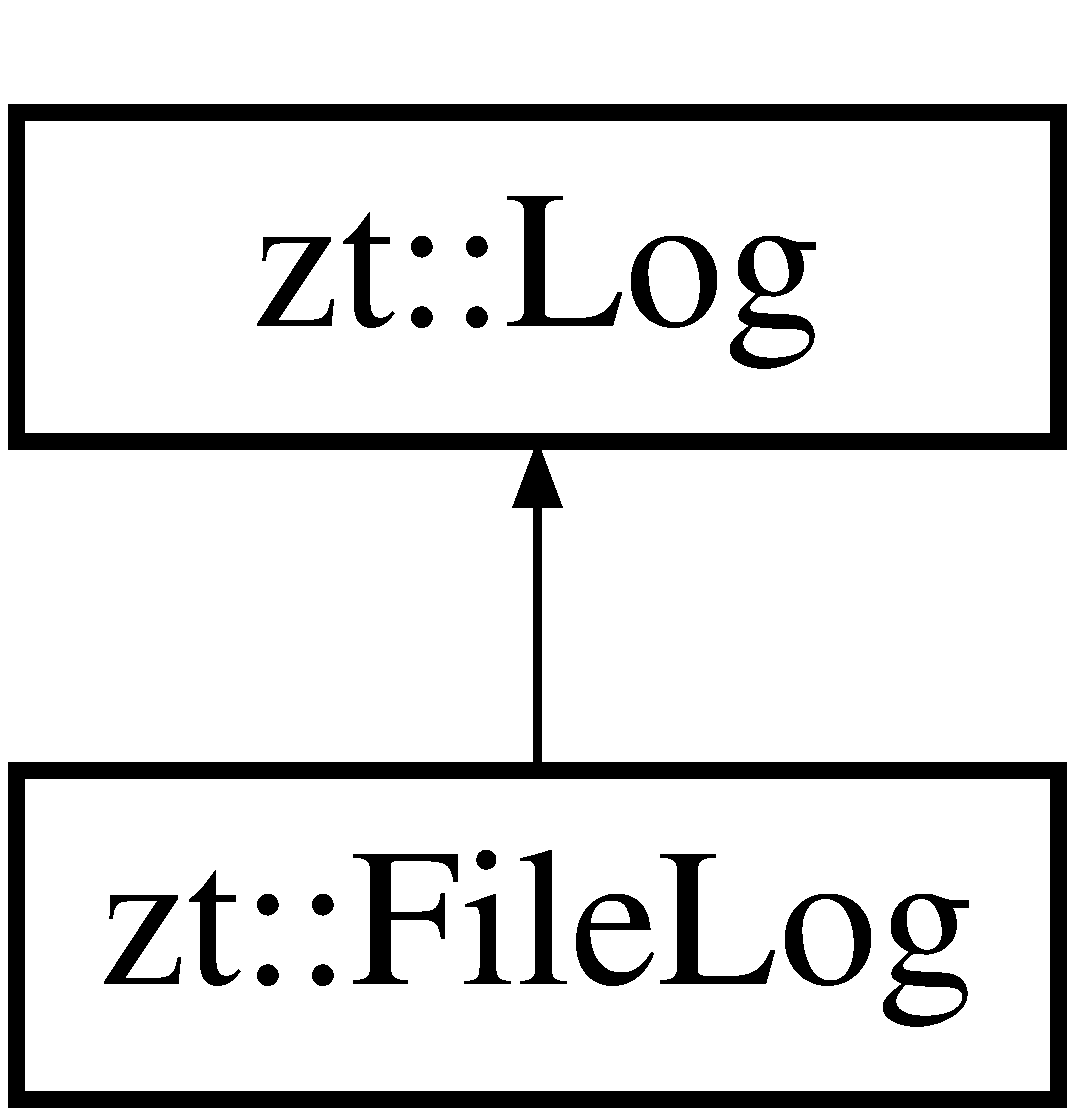
\includegraphics[height=2.000000cm]{classzt_1_1_file_log}
\end{center}
\end{figure}
\subsection*{Public Types}
\begin{DoxyCompactItemize}
\item 
\mbox{\Hypertarget{classzt_1_1_file_log_a9cfc1f53da3e577208c3559c7bf2bc2c}\label{classzt_1_1_file_log_a9cfc1f53da3e577208c3559c7bf2bc2c}} 
enum {\bfseries Mode} \{ {\bfseries K\+E\+E\+P\+\_\+\+P\+R\+E\+V\+I\+O\+U\+S\+\_\+\+L\+OG}, 
{\bfseries R\+E\+M\+O\+V\+E\+\_\+\+P\+R\+E\+V\+I\+O\+U\+S\+\_\+\+L\+OG}
 \}
\end{DoxyCompactItemize}
\subsection*{Public Member Functions}
\begin{DoxyCompactItemize}
\item 
\hyperlink{classzt_1_1_file_log_a9641437081c1f57fb9f439e077dd97f7}{File\+Log} ()
\item 
\hyperlink{classzt_1_1_file_log_ac54d6900bdf714cfb297e066651905a3}{File\+Log} (const std\+::string \&filename, Mode mode=Mode\+::\+K\+E\+E\+P\+\_\+\+P\+R\+E\+V\+I\+O\+U\+S\+\_\+\+L\+OG)
\item 
bool \hyperlink{classzt_1_1_file_log_a4ef54c06277e13646f014d77a62fa2d6}{open} (const std\+::string \&filename, Mode mode=Mode\+::\+K\+E\+E\+P\+\_\+\+P\+R\+E\+V\+I\+O\+U\+S\+\_\+\+L\+OG)
\begin{DoxyCompactList}\small\item\em Open the log file. \end{DoxyCompactList}\item 
\mbox{\Hypertarget{classzt_1_1_file_log_a363d3a84506f56ac0dae23765ec32a04}\label{classzt_1_1_file_log_a363d3a84506f56ac0dae23765ec32a04}} 
void \hyperlink{classzt_1_1_file_log_a363d3a84506f56ac0dae23765ec32a04}{close} ()
\begin{DoxyCompactList}\small\item\em Closes the log file. You won\textquotesingle{}t be able to write after closing it. If you don\textquotesingle{}t call it explicitly it will be called in the destructor. \end{DoxyCompactList}\item 
\mbox{\Hypertarget{classzt_1_1_file_log_a7b17c16a57f5b610416a685f7e9b2bfb}\label{classzt_1_1_file_log_a7b17c16a57f5b610416a685f7e9b2bfb}} 
void {\bfseries log} (Log\+::\+Type type, const std\+::string \&message)
\item 
\mbox{\Hypertarget{classzt_1_1_file_log_a02ae73fbaf82e487d17ca6a6a1462c46}\label{classzt_1_1_file_log_a02ae73fbaf82e487d17ca6a6a1462c46}} 
\hyperlink{classzt_1_1_file_log}{File\+Log} \& {\bfseries operator$<$$<$} (const std\+::string \&message)
\item 
\mbox{\Hypertarget{classzt_1_1_file_log_af578e4259455ae5e304b0dba1f2bb097}\label{classzt_1_1_file_log_af578e4259455ae5e304b0dba1f2bb097}} 
\hyperlink{classzt_1_1_file_log}{File\+Log} \& {\bfseries operator$<$$<$} (const Log\+::\+Type \&type)
\end{DoxyCompactItemize}
\subsection*{Additional Inherited Members}


\subsection{Detailed Description}
Class for logging to a file. 

\subsection{Constructor \& Destructor Documentation}
\mbox{\Hypertarget{classzt_1_1_file_log_a9641437081c1f57fb9f439e077dd97f7}\label{classzt_1_1_file_log_a9641437081c1f57fb9f439e077dd97f7}} 
\index{zt\+::\+File\+Log@{zt\+::\+File\+Log}!File\+Log@{File\+Log}}
\index{File\+Log@{File\+Log}!zt\+::\+File\+Log@{zt\+::\+File\+Log}}
\subsubsection{\texorpdfstring{File\+Log()}{FileLog()}\hspace{0.1cm}{\footnotesize\ttfamily [1/2]}}
{\footnotesize\ttfamily zt\+::\+File\+Log\+::\+File\+Log (\begin{DoxyParamCaption}{ }\end{DoxyParamCaption})}

Constructs a \hyperlink{classzt_1_1_file_log}{File\+Log}. You should open the file before logging using the \hyperlink{classzt_1_1_file_log_a4ef54c06277e13646f014d77a62fa2d6}{open()} method or using the second constructor instead. \mbox{\Hypertarget{classzt_1_1_file_log_ac54d6900bdf714cfb297e066651905a3}\label{classzt_1_1_file_log_ac54d6900bdf714cfb297e066651905a3}} 
\index{zt\+::\+File\+Log@{zt\+::\+File\+Log}!File\+Log@{File\+Log}}
\index{File\+Log@{File\+Log}!zt\+::\+File\+Log@{zt\+::\+File\+Log}}
\subsubsection{\texorpdfstring{File\+Log()}{FileLog()}\hspace{0.1cm}{\footnotesize\ttfamily [2/2]}}
{\footnotesize\ttfamily zt\+::\+File\+Log\+::\+File\+Log (\begin{DoxyParamCaption}\item[{const std\+::string \&}]{filename,  }\item[{Mode}]{mode = {\ttfamily Mode\+:\+:KEEP\+\_\+PREVIOUS\+\_\+LOG} }\end{DoxyParamCaption})}


\begin{DoxyParams}{Parameters}
{\em filename} & Output file. \\
\hline
{\em mode} & If the file already exists you can either keep it or override it. \\
\hline
\end{DoxyParams}


\subsection{Member Function Documentation}
\mbox{\Hypertarget{classzt_1_1_file_log_a4ef54c06277e13646f014d77a62fa2d6}\label{classzt_1_1_file_log_a4ef54c06277e13646f014d77a62fa2d6}} 
\index{zt\+::\+File\+Log@{zt\+::\+File\+Log}!open@{open}}
\index{open@{open}!zt\+::\+File\+Log@{zt\+::\+File\+Log}}
\subsubsection{\texorpdfstring{open()}{open()}}
{\footnotesize\ttfamily bool zt\+::\+File\+Log\+::open (\begin{DoxyParamCaption}\item[{const std\+::string \&}]{filename,  }\item[{Mode}]{mode = {\ttfamily Mode\+:\+:KEEP\+\_\+PREVIOUS\+\_\+LOG} }\end{DoxyParamCaption})}



Open the log file. 


\begin{DoxyParams}{Parameters}
{\em Filename.} & \\
\hline
{\em M\+O\+DE} & If the file already exists you can keep it or you can override it. \\
\hline
\end{DoxyParams}
\begin{DoxyReturn}{Returns}
T\+R\+UE si el archivo está abierto y se puede escribir, si no, F\+A\+L\+SE. 
\end{DoxyReturn}


The documentation for this class was generated from the following file\+:\begin{DoxyCompactItemize}
\item 
include/\+Zelta/\+Core/File\+Log.\+hpp\end{DoxyCompactItemize}

\hypertarget{classzt_1_1_file_not_found_exception}{}\section{zt\+:\+:File\+Not\+Found\+Exception Class Reference}
\label{classzt_1_1_file_not_found_exception}\index{zt\+::\+File\+Not\+Found\+Exception@{zt\+::\+File\+Not\+Found\+Exception}}


Exception throwed when a file is not found.  




{\ttfamily \#include $<$File\+Not\+Found\+Exception.\+hpp$>$}

Inheritance diagram for zt\+:\+:File\+Not\+Found\+Exception\+:\begin{figure}[H]
\begin{center}
\leavevmode
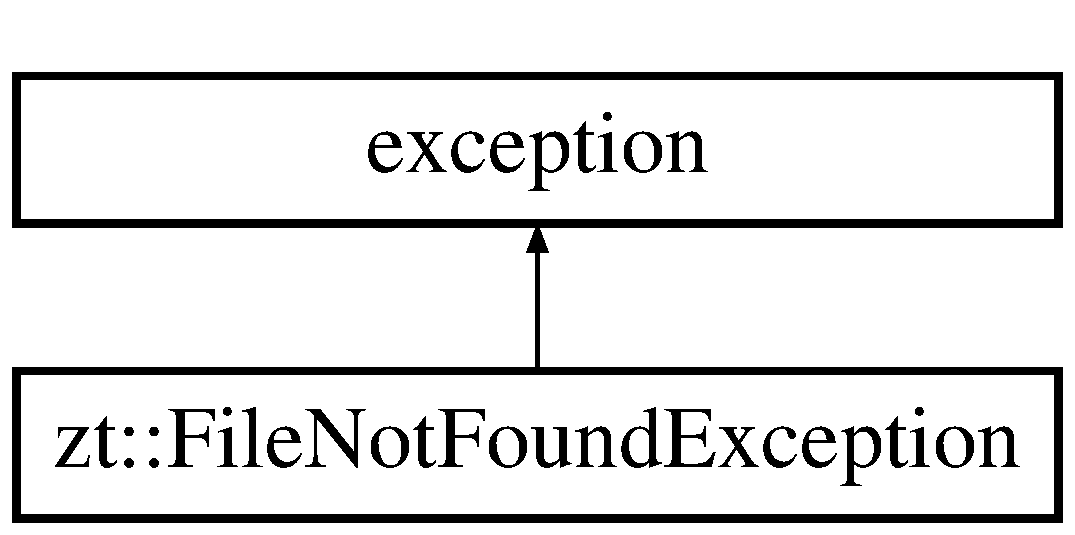
\includegraphics[height=2.000000cm]{classzt_1_1_file_not_found_exception}
\end{center}
\end{figure}
\subsection*{Public Member Functions}
\begin{DoxyCompactItemize}
\item 
\mbox{\Hypertarget{classzt_1_1_file_not_found_exception_a091a0f51ae4994992c0b14dbf2c418e7}\label{classzt_1_1_file_not_found_exception_a091a0f51ae4994992c0b14dbf2c418e7}} 
{\bfseries File\+Not\+Found\+Exception} (const std\+::string \&file\+Name)
\item 
\mbox{\Hypertarget{classzt_1_1_file_not_found_exception_a920c22b2905a4a871d8373543167cadb}\label{classzt_1_1_file_not_found_exception_a920c22b2905a4a871d8373543167cadb}} 
const char $\ast$ {\bfseries what} () const noexcept
\end{DoxyCompactItemize}


\subsection{Detailed Description}
Exception throwed when a file is not found. 

The documentation for this class was generated from the following file\+:\begin{DoxyCompactItemize}
\item 
include/\+Zelta/\+Core/File\+Not\+Found\+Exception.\+hpp\end{DoxyCompactItemize}

\hypertarget{classzt_1_1_font_manager}{}\section{zt\+:\+:Font\+Manager Class Reference}
\label{classzt_1_1_font_manager}\index{zt\+::\+Font\+Manager@{zt\+::\+Font\+Manager}}


Resource manager for sf\+::\+Font.  




{\ttfamily \#include $<$Font\+Manager.\+hpp$>$}

Inheritance diagram for zt\+:\+:Font\+Manager\+:\begin{figure}[H]
\begin{center}
\leavevmode
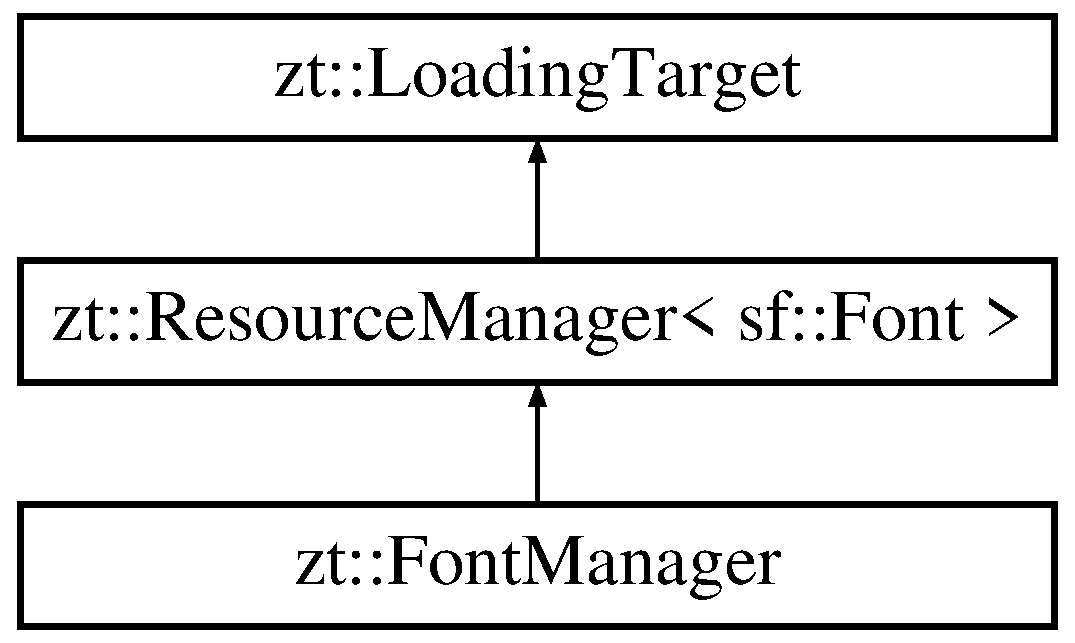
\includegraphics[height=3.000000cm]{classzt_1_1_font_manager}
\end{center}
\end{figure}
\subsection*{Public Member Functions}
\begin{DoxyCompactItemize}
\item 
\mbox{\Hypertarget{classzt_1_1_font_manager_aa6fec447efd9a704bb38996264db7397}\label{classzt_1_1_font_manager_aa6fec447efd9a704bb38996264db7397}} 
virtual void {\bfseries load\+From\+File} (const std\+::string \&name, const std\+::string \&file)
\item 
\mbox{\Hypertarget{classzt_1_1_font_manager_a499f87da8cf45045869b7e018b2ed150}\label{classzt_1_1_font_manager_a499f87da8cf45045869b7e018b2ed150}} 
virtual void {\bfseries load\+From\+Memory} (const std\+::string \&name, const void $\ast$data, std\+::size\+\_\+t size)
\end{DoxyCompactItemize}
\subsection*{Additional Inherited Members}


\subsection{Detailed Description}
Resource manager for sf\+::\+Font. 

The documentation for this class was generated from the following file\+:\begin{DoxyCompactItemize}
\item 
include/\+Zelta/\+Core/Font\+Manager.\+hpp\end{DoxyCompactItemize}

\hypertarget{classzt_1_1_i_mesh}{}\section{zt\+:\+:I\+Mesh$<$ Node\+Type $>$ Class Template Reference}
\label{classzt_1_1_i_mesh}\index{zt\+::\+I\+Mesh$<$ Node\+Type $>$@{zt\+::\+I\+Mesh$<$ Node\+Type $>$}}
\subsection*{Public Member Functions}
\begin{DoxyCompactItemize}
\item 
\mbox{\Hypertarget{classzt_1_1_i_mesh_a88bfc73418c80edbdd6fc4027448a47c}\label{classzt_1_1_i_mesh_a88bfc73418c80edbdd6fc4027448a47c}} 
virtual std\+::vector$<$ Node\+Type $>$ {\bfseries get\+Adjacents} (const Node\+Type \&node) const =0
\item 
\mbox{\Hypertarget{classzt_1_1_i_mesh_a80e2dffb3dfd54075cb4ac9372ceeb96}\label{classzt_1_1_i_mesh_a80e2dffb3dfd54075cb4ac9372ceeb96}} 
virtual float {\bfseries cost} (const Node\+Type \&node1, const Node\+Type \&node2) const =0
\item 
\mbox{\Hypertarget{classzt_1_1_i_mesh_a4a6d526ba6f809e0e6ab6df8549754c7}\label{classzt_1_1_i_mesh_a4a6d526ba6f809e0e6ab6df8549754c7}} 
virtual float {\bfseries estimate} (const Node\+Type \&node1, const Node\+Type \&node2) const =0
\end{DoxyCompactItemize}


The documentation for this class was generated from the following file\+:\begin{DoxyCompactItemize}
\item 
include/\+Zelta/\+A\+I/Pathfinding.\+hpp\end{DoxyCompactItemize}

\hypertarget{classzt_1_1_i_node}{}\section{zt\+:\+:I\+Node Class Reference}
\label{classzt_1_1_i_node}\index{zt\+::\+I\+Node@{zt\+::\+I\+Node}}


The documentation for this class was generated from the following file\+:\begin{DoxyCompactItemize}
\item 
include/\+Zelta/\+A\+I/Pathfinding.\+hpp\end{DoxyCompactItemize}

\hypertarget{classzt_1_1tiled_1_1_layer}{}\section{zt\+:\+:tiled\+:\+:Layer Class Reference}
\label{classzt_1_1tiled_1_1_layer}\index{zt\+::tiled\+::\+Layer@{zt\+::tiled\+::\+Layer}}
\subsection*{Public Member Functions}
\begin{DoxyCompactItemize}
\item 
\mbox{\Hypertarget{classzt_1_1tiled_1_1_layer_a13adb1b0b39d84449c87459dd975977e}\label{classzt_1_1tiled_1_1_layer_a13adb1b0b39d84449c87459dd975977e}} 
{\bfseries Layer} (const std\+::wstring \&name, int width, int height)
\item 
\mbox{\Hypertarget{classzt_1_1tiled_1_1_layer_a1ea8418548abbc6af971692debe2f960}\label{classzt_1_1tiled_1_1_layer_a1ea8418548abbc6af971692debe2f960}} 
int {\bfseries get\+Width} () const
\item 
\mbox{\Hypertarget{classzt_1_1tiled_1_1_layer_aa492ded76f951bfce818dd4a10b35133}\label{classzt_1_1tiled_1_1_layer_aa492ded76f951bfce818dd4a10b35133}} 
int {\bfseries get\+Height} () const
\item 
\mbox{\Hypertarget{classzt_1_1tiled_1_1_layer_a0e0978346385a32ccd397ce260179644}\label{classzt_1_1tiled_1_1_layer_a0e0978346385a32ccd397ce260179644}} 
std\+::wstring {\bfseries get\+Name} () const
\item 
\mbox{\Hypertarget{classzt_1_1tiled_1_1_layer_ae3275e8593025156d90addcaa424f447}\label{classzt_1_1tiled_1_1_layer_ae3275e8593025156d90addcaa424f447}} 
\hyperlink{classzt_1_1tiled_1_1_tile}{Tile} \& {\bfseries operator\mbox{[}$\,$\mbox{]}} (int index)
\item 
\mbox{\Hypertarget{classzt_1_1tiled_1_1_layer_a4d99e5bcfc8ab9d463822de93dfa6cbf}\label{classzt_1_1tiled_1_1_layer_a4d99e5bcfc8ab9d463822de93dfa6cbf}} 
\hyperlink{classzt_1_1tiled_1_1_tile}{Tile} \& {\bfseries at} (int x, int y)
\item 
\mbox{\Hypertarget{classzt_1_1tiled_1_1_layer_a3d02819c7de5dba5028b186c09ebf411}\label{classzt_1_1tiled_1_1_layer_a3d02819c7de5dba5028b186c09ebf411}} 
void {\bfseries add\+Tile} (const \hyperlink{classzt_1_1tiled_1_1_tile}{Tile} \&tile)
\end{DoxyCompactItemize}
\subsection*{Protected Attributes}
\begin{DoxyCompactItemize}
\item 
\mbox{\Hypertarget{classzt_1_1tiled_1_1_layer_a65bd471d225baa753d3cb7e76800a7f1}\label{classzt_1_1tiled_1_1_layer_a65bd471d225baa753d3cb7e76800a7f1}} 
std\+::vector$<$ \hyperlink{classzt_1_1tiled_1_1_tile}{Tile} $>$ {\bfseries tiles}
\item 
\mbox{\Hypertarget{classzt_1_1tiled_1_1_layer_accf8e58c7bf6e047d93af28baa793fe2}\label{classzt_1_1tiled_1_1_layer_accf8e58c7bf6e047d93af28baa793fe2}} 
std\+::wstring {\bfseries name}
\item 
\mbox{\Hypertarget{classzt_1_1tiled_1_1_layer_ac0465586e45f5cb485c45599763e3b7d}\label{classzt_1_1tiled_1_1_layer_ac0465586e45f5cb485c45599763e3b7d}} 
int {\bfseries width}
\item 
\mbox{\Hypertarget{classzt_1_1tiled_1_1_layer_a3f98f0840078a3713ada2e756b05da57}\label{classzt_1_1tiled_1_1_layer_a3f98f0840078a3713ada2e756b05da57}} 
int {\bfseries height}
\end{DoxyCompactItemize}


The documentation for this class was generated from the following file\+:\begin{DoxyCompactItemize}
\item 
include/\+Zelta/\+Tile\+Engine/\+Tiled\+Loader/Layer.\+hpp\end{DoxyCompactItemize}

\hypertarget{classzt_1_1_loading_target}{}\section{zt\+:\+:Loading\+Target Class Reference}
\label{classzt_1_1_loading_target}\index{zt\+::\+Loading\+Target@{zt\+::\+Loading\+Target}}


Base class for resource containers. It represents something you can load things into.  




{\ttfamily \#include $<$Loading\+Target.\+hpp$>$}

Inheritance diagram for zt\+:\+:Loading\+Target\+:\begin{figure}[H]
\begin{center}
\leavevmode
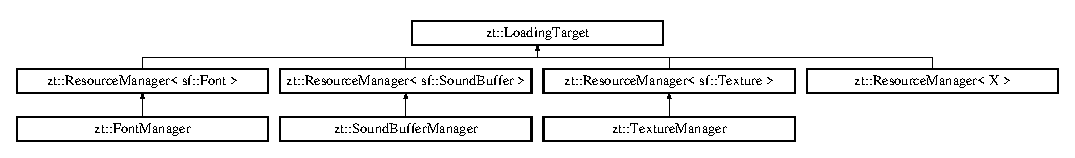
\includegraphics[height=1.673307cm]{classzt_1_1_loading_target}
\end{center}
\end{figure}
\subsection*{Public Member Functions}
\begin{DoxyCompactItemize}
\item 
\mbox{\Hypertarget{classzt_1_1_loading_target_ab83041e95e2f3584af0e2ce726528246}\label{classzt_1_1_loading_target_ab83041e95e2f3584af0e2ce726528246}} 
virtual void {\bfseries load\+From\+File} (const std\+::string \&name, const std\+::string \&path)=0
\item 
\mbox{\Hypertarget{classzt_1_1_loading_target_a9f5edbd26bb353be24d7cf0c862f62b3}\label{classzt_1_1_loading_target_a9f5edbd26bb353be24d7cf0c862f62b3}} 
virtual void {\bfseries load\+From\+Memory} (const std\+::string \&name, const void $\ast$data, std\+::size\+\_\+t size)=0
\item 
\mbox{\Hypertarget{classzt_1_1_loading_target_afa0e97a98e68d1b55689498e15513d9e}\label{classzt_1_1_loading_target_afa0e97a98e68d1b55689498e15513d9e}} 
virtual void {\bfseries release} (const std\+::string \&name)=0
\item 
\mbox{\Hypertarget{classzt_1_1_loading_target_a1e325d02640f2f80d1a11fb06d9cc154}\label{classzt_1_1_loading_target_a1e325d02640f2f80d1a11fb06d9cc154}} 
virtual const std\+::string \& {\bfseries get\+Name} () const =0
\item 
\mbox{\Hypertarget{classzt_1_1_loading_target_a90f011dd3aac3369ada59a3776e8e598}\label{classzt_1_1_loading_target_a90f011dd3aac3369ada59a3776e8e598}} 
virtual void {\bfseries pendant} (const std\+::string \&name, \hyperlink{classzt_1_1_resource_provider}{Resource\+Provider} \&provider)=0
\item 
\mbox{\Hypertarget{classzt_1_1_loading_target_aef330cfe486b1927b7b4c155b36043f2}\label{classzt_1_1_loading_target_aef330cfe486b1927b7b4c155b36043f2}} 
virtual void {\bfseries not\+Pendant} (const std\+::string \&name)=0
\item 
\mbox{\Hypertarget{classzt_1_1_loading_target_afb1845a9d49b2d5f0e01d1688405a479}\label{classzt_1_1_loading_target_afb1845a9d49b2d5f0e01d1688405a479}} 
virtual bool {\bfseries exists} (const std\+::string \&name) const =0
\item 
\mbox{\Hypertarget{classzt_1_1_loading_target_a42246fda572f1c00c52e3fed55209d0b}\label{classzt_1_1_loading_target_a42246fda572f1c00c52e3fed55209d0b}} 
virtual bool {\bfseries is\+Loaded} (const std\+::string \&name) const =0
\end{DoxyCompactItemize}


\subsection{Detailed Description}
Base class for resource containers. It represents something you can load things into. 

The documentation for this class was generated from the following file\+:\begin{DoxyCompactItemize}
\item 
include/\+Zelta/\+Core/Loading\+Target.\+hpp\end{DoxyCompactItemize}

\hypertarget{classzt_1_1_log}{}\section{zt\+:\+:Log Class Reference}
\label{classzt_1_1_log}\index{zt\+::\+Log@{zt\+::\+Log}}


Base class for logging.  




{\ttfamily \#include $<$Log.\+hpp$>$}

Inheritance diagram for zt\+:\+:Log\+:\begin{figure}[H]
\begin{center}
\leavevmode
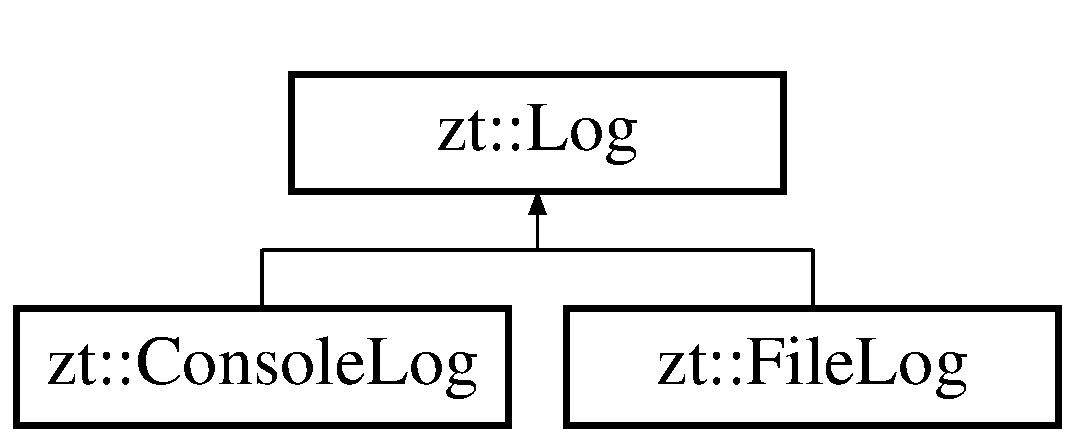
\includegraphics[height=2.000000cm]{classzt_1_1_log}
\end{center}
\end{figure}
\subsection*{Public Types}
\begin{DoxyCompactItemize}
\item 
\mbox{\Hypertarget{classzt_1_1_log_aec3ae67596b29202b7154380cbdb3ae9}\label{classzt_1_1_log_aec3ae67596b29202b7154380cbdb3ae9}} 
enum {\bfseries Type} \{ {\bfseries E\+R\+R\+OR}, 
{\bfseries W\+A\+R\+N\+I\+NG}, 
{\bfseries I\+N\+FO}, 
{\bfseries S\+U\+C\+C\+E\+SS}
 \}
\end{DoxyCompactItemize}
\subsection*{Public Member Functions}
\begin{DoxyCompactItemize}
\item 
\mbox{\Hypertarget{classzt_1_1_log_ad2cf7a53c6646b187dca65cbcf667d6c}\label{classzt_1_1_log_ad2cf7a53c6646b187dca65cbcf667d6c}} 
virtual void {\bfseries log} (Log\+::\+Type type, const std\+::string \&message)=0
\item 
\mbox{\Hypertarget{classzt_1_1_log_a07977fb4dc29aea94383c5700f72492a}\label{classzt_1_1_log_a07977fb4dc29aea94383c5700f72492a}} 
virtual void {\bfseries error} (const std\+::string \&message)
\item 
\mbox{\Hypertarget{classzt_1_1_log_ac6e0e1586ccf2239136df6e1a98e2b8e}\label{classzt_1_1_log_ac6e0e1586ccf2239136df6e1a98e2b8e}} 
virtual void {\bfseries info} (const std\+::string \&message)
\item 
\mbox{\Hypertarget{classzt_1_1_log_a11094b09c3e1d6d60ca501f4889fe266}\label{classzt_1_1_log_a11094b09c3e1d6d60ca501f4889fe266}} 
virtual void {\bfseries warning} (const std\+::string \&message)
\item 
\mbox{\Hypertarget{classzt_1_1_log_a00f9214b32a771bc11a08d2fac88dea7}\label{classzt_1_1_log_a00f9214b32a771bc11a08d2fac88dea7}} 
virtual void {\bfseries success} (const std\+::string \&message)
\end{DoxyCompactItemize}
\subsection*{Protected Attributes}
\begin{DoxyCompactItemize}
\item 
\mbox{\Hypertarget{classzt_1_1_log_a95116d9d99af0b6196d17819b34f42d9}\label{classzt_1_1_log_a95116d9d99af0b6196d17819b34f42d9}} 
Type {\bfseries last\+Mode}
\end{DoxyCompactItemize}


\subsection{Detailed Description}
Base class for logging. 

You may find useful the Z\+E\+L\+T\+A\+\_\+\+L\+O\+G\+\_\+\+W\+A\+R\+N\+I\+NG(...), Z\+E\+L\+T\+A\+\_\+\+L\+O\+G\+\_\+\+I\+N\+FO(...), Z\+E\+L\+T\+A\+\_\+\+L\+O\+G\+\_\+\+E\+R\+R\+OR(...) and Z\+E\+L\+T\+A\+\_\+\+L\+O\+G\+\_\+\+S\+U\+C\+C\+E\+SS(...) directives that only logs when the Z\+E\+L\+T\+A\+L\+I\+B\+\_\+\+D\+E\+B\+UG directive si defined. 

The documentation for this class was generated from the following file\+:\begin{DoxyCompactItemize}
\item 
include/\+Zelta/\+Core/Log.\+hpp\end{DoxyCompactItemize}

\hypertarget{classzt_1_1tiled_1_1_map}{}\section{zt\+:\+:tiled\+:\+:Map Class Reference}
\label{classzt_1_1tiled_1_1_map}\index{zt\+::tiled\+::\+Map@{zt\+::tiled\+::\+Map}}
\subsection*{Public Types}
\begin{DoxyCompactItemize}
\item 
\mbox{\Hypertarget{classzt_1_1tiled_1_1_map_a9f333709d2b355070a8ba573af0133a5}\label{classzt_1_1tiled_1_1_map_a9f333709d2b355070a8ba573af0133a5}} 
enum {\bfseries Orientation} \{ {\bfseries Orthogonal}, 
{\bfseries Isometric}, 
{\bfseries Staggered}, 
{\bfseries Hexagonal}
 \}
\end{DoxyCompactItemize}
\subsection*{Public Member Functions}
\begin{DoxyCompactItemize}
\item 
\mbox{\Hypertarget{classzt_1_1tiled_1_1_map_aea345c396798c0325610d6d3719bd4ca}\label{classzt_1_1tiled_1_1_map_aea345c396798c0325610d6d3719bd4ca}} 
{\bfseries Map} (int width, int height, int tile\+Width, int tile\+Height, Orientation orientation)
\item 
\mbox{\Hypertarget{classzt_1_1tiled_1_1_map_ab159d99e9fa5c9665e641ecddc69849d}\label{classzt_1_1tiled_1_1_map_ab159d99e9fa5c9665e641ecddc69849d}} 
int {\bfseries get\+Width} () const
\item 
\mbox{\Hypertarget{classzt_1_1tiled_1_1_map_a97c432d47f009bd961c39ff24a0aec32}\label{classzt_1_1tiled_1_1_map_a97c432d47f009bd961c39ff24a0aec32}} 
int {\bfseries get\+Height} () const
\item 
\mbox{\Hypertarget{classzt_1_1tiled_1_1_map_a318c7fab2dd0054662b5743a99a5b183}\label{classzt_1_1tiled_1_1_map_a318c7fab2dd0054662b5743a99a5b183}} 
int {\bfseries get\+Tile\+Width} () const
\item 
\mbox{\Hypertarget{classzt_1_1tiled_1_1_map_a8317f25e7c01eeba26929bab350a6f61}\label{classzt_1_1tiled_1_1_map_a8317f25e7c01eeba26929bab350a6f61}} 
int {\bfseries get\+Tile\+Height} () const
\item 
\mbox{\Hypertarget{classzt_1_1tiled_1_1_map_abeae78f4a66d89e7c458d9b842de01b7}\label{classzt_1_1tiled_1_1_map_abeae78f4a66d89e7c458d9b842de01b7}} 
Orientation {\bfseries get\+Orientation} () const
\item 
\mbox{\Hypertarget{classzt_1_1tiled_1_1_map_ab0cd802b94079f5322ad8584fe22ae91}\label{classzt_1_1tiled_1_1_map_ab0cd802b94079f5322ad8584fe22ae91}} 
void {\bfseries add\+Layer} (const \hyperlink{classzt_1_1tiled_1_1_layer}{Layer} \&layer)
\item 
\mbox{\Hypertarget{classzt_1_1tiled_1_1_map_ab5735ce37acd2c58f7aa855e97123258}\label{classzt_1_1tiled_1_1_map_ab5735ce37acd2c58f7aa855e97123258}} 
std\+::vector$<$ \hyperlink{classzt_1_1tiled_1_1_layer}{Layer} $>$ \& {\bfseries get\+Layers} ()
\item 
\mbox{\Hypertarget{classzt_1_1tiled_1_1_map_a4061885e6af9816c053da0415bb6be48}\label{classzt_1_1tiled_1_1_map_a4061885e6af9816c053da0415bb6be48}} 
void {\bfseries add\+Object\+Layer} (const \hyperlink{classzt_1_1tiled_1_1_object_layer}{Object\+Layer} \&object\+Layer)
\item 
\mbox{\Hypertarget{classzt_1_1tiled_1_1_map_abe765796c91b94dfa089ef7547015582}\label{classzt_1_1tiled_1_1_map_abe765796c91b94dfa089ef7547015582}} 
std\+::vector$<$ \hyperlink{classzt_1_1tiled_1_1_object_layer}{Object\+Layer} $>$ \& {\bfseries get\+Object\+Layers} ()
\end{DoxyCompactItemize}
\subsection*{Protected Attributes}
\begin{DoxyCompactItemize}
\item 
\mbox{\Hypertarget{classzt_1_1tiled_1_1_map_a7b065317a42d6a98ae275182729a59d5}\label{classzt_1_1tiled_1_1_map_a7b065317a42d6a98ae275182729a59d5}} 
int {\bfseries width}
\item 
\mbox{\Hypertarget{classzt_1_1tiled_1_1_map_a9c29ddcafc21491f8520e1b0f99e9c39}\label{classzt_1_1tiled_1_1_map_a9c29ddcafc21491f8520e1b0f99e9c39}} 
int {\bfseries height}
\item 
\mbox{\Hypertarget{classzt_1_1tiled_1_1_map_a693997ec67f196932c2b5423164cd39e}\label{classzt_1_1tiled_1_1_map_a693997ec67f196932c2b5423164cd39e}} 
int {\bfseries tile\+Width}
\item 
\mbox{\Hypertarget{classzt_1_1tiled_1_1_map_a8777e8e66e02ecef64559d1d7e319ec5}\label{classzt_1_1tiled_1_1_map_a8777e8e66e02ecef64559d1d7e319ec5}} 
int {\bfseries tile\+Height}
\item 
\mbox{\Hypertarget{classzt_1_1tiled_1_1_map_a35cbc297da3e7c99935ef3d05a12d1eb}\label{classzt_1_1tiled_1_1_map_a35cbc297da3e7c99935ef3d05a12d1eb}} 
Orientation {\bfseries orientation}
\item 
\mbox{\Hypertarget{classzt_1_1tiled_1_1_map_a655966027df4fb07327780d944f47373}\label{classzt_1_1tiled_1_1_map_a655966027df4fb07327780d944f47373}} 
std\+::vector$<$ \hyperlink{classzt_1_1tiled_1_1_layer}{Layer} $>$ {\bfseries layers}
\item 
\mbox{\Hypertarget{classzt_1_1tiled_1_1_map_aa511c68193fd8a6cb627ce65378f6e5e}\label{classzt_1_1tiled_1_1_map_aa511c68193fd8a6cb627ce65378f6e5e}} 
std\+::vector$<$ \hyperlink{classzt_1_1tiled_1_1_object_layer}{Object\+Layer} $>$ {\bfseries object\+Layers}
\end{DoxyCompactItemize}


The documentation for this class was generated from the following file\+:\begin{DoxyCompactItemize}
\item 
include/\+Zelta/\+Tile\+Engine/\+Tiled\+Loader/Map.\+hpp\end{DoxyCompactItemize}

\hypertarget{classzt_1_1_nestable_clock}{}\section{zt\+:\+:Nestable\+Clock Class Reference}
\label{classzt_1_1_nestable_clock}\index{zt\+::\+Nestable\+Clock@{zt\+::\+Nestable\+Clock}}
Inheritance diagram for zt\+:\+:Nestable\+Clock\+:\begin{figure}[H]
\begin{center}
\leavevmode
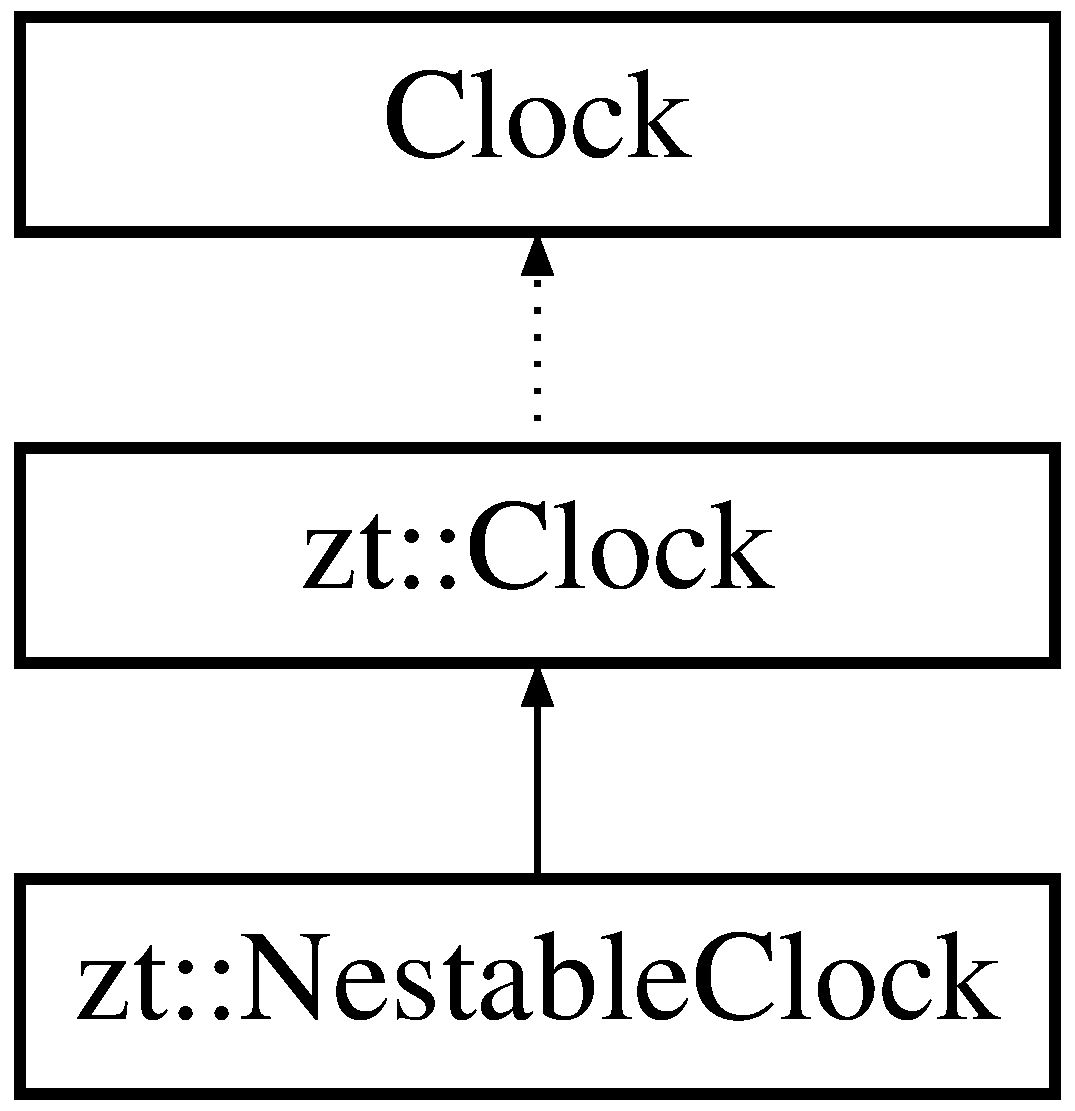
\includegraphics[height=3.000000cm]{classzt_1_1_nestable_clock}
\end{center}
\end{figure}
\subsection*{Public Member Functions}
\begin{DoxyCompactItemize}
\item 
\mbox{\Hypertarget{classzt_1_1_nestable_clock_afc262bba7ae3fedec80f58d8daf74575}\label{classzt_1_1_nestable_clock_afc262bba7ae3fedec80f58d8daf74575}} 
void {\bfseries add\+Clock} (\hyperlink{classzt_1_1_nestable_clock}{zt\+::\+Nestable\+Clock} \&clock)
\item 
\mbox{\Hypertarget{classzt_1_1_nestable_clock_a429fd96903819349981f10523b1a45b6}\label{classzt_1_1_nestable_clock_a429fd96903819349981f10523b1a45b6}} 
void {\bfseries pause} ()
\item 
\mbox{\Hypertarget{classzt_1_1_nestable_clock_ae157673580027b82b54964f1380f5b9d}\label{classzt_1_1_nestable_clock_ae157673580027b82b54964f1380f5b9d}} 
void {\bfseries resume} ()
\item 
\mbox{\Hypertarget{classzt_1_1_nestable_clock_a0c7d3b6e91465e14cbeab841b888d55b}\label{classzt_1_1_nestable_clock_a0c7d3b6e91465e14cbeab841b888d55b}} 
bool {\bfseries is\+Locked} () const
\item 
\mbox{\Hypertarget{classzt_1_1_nestable_clock_a00ef4ad0179e820e8e0d960acec19e2f}\label{classzt_1_1_nestable_clock_a00ef4ad0179e820e8e0d960acec19e2f}} 
\hyperlink{classzt_1_1_nestable_clock}{Nestable\+Clock} \& {\bfseries lock} ()
\end{DoxyCompactItemize}


The documentation for this class was generated from the following file\+:\begin{DoxyCompactItemize}
\item 
include/\+Zelta/\+Core/Nestable\+Clock.\+hpp\end{DoxyCompactItemize}

\hypertarget{classzt_1_1tiled_1_1_object}{}\section{zt\+:\+:tiled\+:\+:Object Class Reference}
\label{classzt_1_1tiled_1_1_object}\index{zt\+::tiled\+::\+Object@{zt\+::tiled\+::\+Object}}
\subsection*{Public Member Functions}
\begin{DoxyCompactItemize}
\item 
\mbox{\Hypertarget{classzt_1_1tiled_1_1_object_a38cb0a9040104272f100723e19ee2d1f}\label{classzt_1_1tiled_1_1_object_a38cb0a9040104272f100723e19ee2d1f}} 
{\bfseries Object} (int id, const std\+::wstring \&name, const std\+::wstring \&type, int x, int y, int gid)
\item 
\mbox{\Hypertarget{classzt_1_1tiled_1_1_object_a4463f1634e0c0caf10ab1e8d2d7fea5f}\label{classzt_1_1tiled_1_1_object_a4463f1634e0c0caf10ab1e8d2d7fea5f}} 
{\bfseries Object} (int id, const std\+::wstring \&name, const std\+::wstring \&type, int x, int y)
\item 
\mbox{\Hypertarget{classzt_1_1tiled_1_1_object_ad4edde1dde628b11a563361c4f27d85c}\label{classzt_1_1tiled_1_1_object_ad4edde1dde628b11a563361c4f27d85c}} 
int {\bfseries get\+Id} () const
\item 
\mbox{\Hypertarget{classzt_1_1tiled_1_1_object_a3e0a50131d3a736d618433bd2952db3d}\label{classzt_1_1tiled_1_1_object_a3e0a50131d3a736d618433bd2952db3d}} 
const std\+::wstring \& {\bfseries get\+Name} () const
\item 
\mbox{\Hypertarget{classzt_1_1tiled_1_1_object_ad6507d7d2869bccc17a2f929cb1e5c08}\label{classzt_1_1tiled_1_1_object_ad6507d7d2869bccc17a2f929cb1e5c08}} 
const std\+::wstring \& {\bfseries get\+Type} () const
\item 
\mbox{\Hypertarget{classzt_1_1tiled_1_1_object_abd81c25aa43deb1aed520b290db126df}\label{classzt_1_1tiled_1_1_object_abd81c25aa43deb1aed520b290db126df}} 
int {\bfseries getX} () const
\item 
\mbox{\Hypertarget{classzt_1_1tiled_1_1_object_a1eb3865ba23cd299101861583d692856}\label{classzt_1_1tiled_1_1_object_a1eb3865ba23cd299101861583d692856}} 
int {\bfseries getY} () const
\item 
\mbox{\Hypertarget{classzt_1_1tiled_1_1_object_a6cad5d27d93c4dc8b2c1779029f11cd1}\label{classzt_1_1tiled_1_1_object_a6cad5d27d93c4dc8b2c1779029f11cd1}} 
int {\bfseries get\+G\+ID} () const
\item 
\mbox{\Hypertarget{classzt_1_1tiled_1_1_object_aa2d833f560921209b0a7c809c5abbcc4}\label{classzt_1_1tiled_1_1_object_aa2d833f560921209b0a7c809c5abbcc4}} 
bool {\bfseries is\+Tile} () const
\end{DoxyCompactItemize}


The documentation for this class was generated from the following file\+:\begin{DoxyCompactItemize}
\item 
include/\+Zelta/\+Tile\+Engine/\+Tiled\+Loader/Object.\+hpp\end{DoxyCompactItemize}

\hypertarget{classzt_1_1tiled_1_1_object_layer}{}\section{zt\+:\+:tiled\+:\+:Object\+Layer Class Reference}
\label{classzt_1_1tiled_1_1_object_layer}\index{zt\+::tiled\+::\+Object\+Layer@{zt\+::tiled\+::\+Object\+Layer}}
\subsection*{Public Member Functions}
\begin{DoxyCompactItemize}
\item 
\mbox{\Hypertarget{classzt_1_1tiled_1_1_object_layer_ae946042ce79a6672304d2bf96b06223a}\label{classzt_1_1tiled_1_1_object_layer_ae946042ce79a6672304d2bf96b06223a}} 
{\bfseries Object\+Layer} (const std\+::wstring \&name)
\item 
\mbox{\Hypertarget{classzt_1_1tiled_1_1_object_layer_aa9876d979c17fd3cb87673b87949657f}\label{classzt_1_1tiled_1_1_object_layer_aa9876d979c17fd3cb87673b87949657f}} 
void {\bfseries add\+Object} (const \hyperlink{classzt_1_1tiled_1_1_object}{Object} \&object)
\item 
\mbox{\Hypertarget{classzt_1_1tiled_1_1_object_layer_add151e3bd53f59f41189068e2353f3c2}\label{classzt_1_1tiled_1_1_object_layer_add151e3bd53f59f41189068e2353f3c2}} 
int {\bfseries size} () const
\item 
\mbox{\Hypertarget{classzt_1_1tiled_1_1_object_layer_a342f9402bce1aa03c51f3a1cae719105}\label{classzt_1_1tiled_1_1_object_layer_a342f9402bce1aa03c51f3a1cae719105}} 
\hyperlink{classzt_1_1tiled_1_1_object}{Object} \& {\bfseries operator\mbox{[}$\,$\mbox{]}} (int index)
\item 
\mbox{\Hypertarget{classzt_1_1tiled_1_1_object_layer_a2523d73c57790290840a8ad113988188}\label{classzt_1_1tiled_1_1_object_layer_a2523d73c57790290840a8ad113988188}} 
const std\+::wstring \& {\bfseries get\+Name} () const
\end{DoxyCompactItemize}


The documentation for this class was generated from the following file\+:\begin{DoxyCompactItemize}
\item 
include/\+Zelta/\+Tile\+Engine/\+Tiled\+Loader/Object\+Layer.\+hpp\end{DoxyCompactItemize}

\hypertarget{classzt_1_1_package}{}\section{zt\+:\+:Package Class Reference}
\label{classzt_1_1_package}\index{zt\+::\+Package@{zt\+::\+Package}}


The \hyperlink{classzt_1_1_package}{Package} class allows you to store all your assets (images, sounds, fonts) in the same file. The class also lets you load those files from the package easily.  




{\ttfamily \#include $<$Package.\+hpp$>$}

\subsection*{Public Member Functions}
\begin{DoxyCompactItemize}
\item 
void \hyperlink{classzt_1_1_package_a985b5fd2f225911709782ec42ea8dc48}{create} (const std\+::string \&file, unsigned int compression=C\+O\+M\+P\+R\+E\+S\+S\+I\+O\+N\+\_\+\+N\+O\+NE)
\begin{DoxyCompactList}\small\item\em Creates a new empty package. \end{DoxyCompactList}\item 
void \hyperlink{classzt_1_1_package_a30d7195cbd7b4856dda6207fd8ec785b}{open} (const std\+::string \&file)
\begin{DoxyCompactList}\small\item\em Opens an existing package. \end{DoxyCompactList}\item 
void \hyperlink{classzt_1_1_package_a5410213f58e0f08e648d6424474e0a5d}{add\+File} (const std\+::string \&input, const std\+::string \&target)
\begin{DoxyCompactList}\small\item\em Adds a file to the package. \end{DoxyCompactList}\item 
void \hyperlink{classzt_1_1_package_a6f528593a7a56b9d2c7ec6df0a6b2bb2}{add\+Directory} (const std\+::string \&directory)
\begin{DoxyCompactList}\small\item\em Adds the content of a directory to the package. \end{DoxyCompactList}\item 
void \hyperlink{classzt_1_1_package_af62e37955ffe46a4c37cd76c99405763}{remove\+File} (const std\+::string \&file)
\begin{DoxyCompactList}\small\item\em Removes a file from the package. This is an expensive task which involves reading the whole package and writing it again without the removed file. \end{DoxyCompactList}\item 
std\+::vector$<$ std\+::string $>$ \hyperlink{classzt_1_1_package_a9454a5a20192952e1d4d2c0ef9e434f4}{get\+Names} () const
\item 
std\+::vector$<$ uint8\+\_\+t $>$ \hyperlink{classzt_1_1_package_ab30b4acb16a680075b9d61de978181f4}{get\+File\+Data} (const std\+::string \&file)
\item 
\mbox{\Hypertarget{classzt_1_1_package_a33d762728678ba4b1769cf99440e54bc}\label{classzt_1_1_package_a33d762728678ba4b1769cf99440e54bc}} 
std\+::string {\bfseries get\+File\+Data\+As\+String} (const std\+::string \&file)
\item 
unsigned long \hyperlink{classzt_1_1_package_a5c8234b81f3076072f5284a257bf0b51}{get\+File\+Size} (const std\+::string \&file)
\end{DoxyCompactItemize}
\subsection*{Static Public Attributes}
\begin{DoxyCompactItemize}
\item 
\mbox{\Hypertarget{classzt_1_1_package_affccb63e5c40c8ab8cd8a4bab5db6914}\label{classzt_1_1_package_affccb63e5c40c8ab8cd8a4bab5db6914}} 
static const unsigned int {\bfseries C\+O\+M\+P\+R\+E\+S\+S\+I\+O\+N\+\_\+\+N\+O\+NE} = 0
\end{DoxyCompactItemize}
\subsection*{Protected Attributes}
\begin{DoxyCompactItemize}
\item 
\mbox{\Hypertarget{classzt_1_1_package_a6937a1bdbb54efd3dd0184590f72a038}\label{classzt_1_1_package_a6937a1bdbb54efd3dd0184590f72a038}} 
std\+::fstream {\bfseries file}
\item 
\mbox{\Hypertarget{classzt_1_1_package_a178f1e16598632e9a28a36c244afadc8}\label{classzt_1_1_package_a178f1e16598632e9a28a36c244afadc8}} 
std\+::string {\bfseries package\+Name}
\item 
\mbox{\Hypertarget{classzt_1_1_package_aed3f124a5138a835ab59d001fd24b8bf}\label{classzt_1_1_package_aed3f124a5138a835ab59d001fd24b8bf}} 
std\+::map$<$ std\+::string, \hyperlink{classzt_1_1_package_file_info}{Package\+File\+Info} $>$ {\bfseries file\+Index}
\item 
\mbox{\Hypertarget{classzt_1_1_package_a06cb77eccd578fe53a04d9b8b9b0c002}\label{classzt_1_1_package_a06cb77eccd578fe53a04d9b8b9b0c002}} 
const unsigned int {\bfseries N\+A\+M\+E\+\_\+\+B\+Y\+T\+ES} = 512
\item 
\mbox{\Hypertarget{classzt_1_1_package_ace3614899778aca2fb25bd0cf1bacb8f}\label{classzt_1_1_package_ace3614899778aca2fb25bd0cf1bacb8f}} 
const unsigned int {\bfseries S\+I\+Z\+E\+\_\+\+B\+Y\+T\+ES} = 8
\item 
\mbox{\Hypertarget{classzt_1_1_package_a02b53b1351ab587787171e9d4a80a424}\label{classzt_1_1_package_a02b53b1351ab587787171e9d4a80a424}} 
const unsigned int {\bfseries V\+E\+R\+S\+I\+ON} = 1
\item 
\mbox{\Hypertarget{classzt_1_1_package_a0a744c3d635b242b2312465822b59dbc}\label{classzt_1_1_package_a0a744c3d635b242b2312465822b59dbc}} 
const char $\ast$ {\bfseries M\+A\+G\+I\+C\+\_\+\+N\+U\+M\+B\+ER} = \char`\"{}Z\+P\+KG\char`\"{}
\end{DoxyCompactItemize}


\subsection{Detailed Description}
The \hyperlink{classzt_1_1_package}{Package} class allows you to store all your assets (images, sounds, fonts) in the same file. The class also lets you load those files from the package easily. 

The package use a custom format called Z\+P\+KG (Zelta\+Lib \hyperlink{classzt_1_1_package}{Package}). A Z\+P\+KG file has a 12 bytes header. -\/\+The first four bytes are the magic number (Z\+P\+KG codified in A\+S\+C\+II). -\/\+The next four bytes represent the version of the format (1, at the moment). -\/\+The last four bytes represent the compression used. At the moment this library does not compress the data (a zero is written).

After the header, we can have zero or more files stored in the package. Each file is composed of a header and the actual data. The header takes 8 bytes to represent the file size and 512 more bytes to represent the file name and path. 

\subsection{Member Function Documentation}
\mbox{\Hypertarget{classzt_1_1_package_a6f528593a7a56b9d2c7ec6df0a6b2bb2}\label{classzt_1_1_package_a6f528593a7a56b9d2c7ec6df0a6b2bb2}} 
\index{zt\+::\+Package@{zt\+::\+Package}!add\+Directory@{add\+Directory}}
\index{add\+Directory@{add\+Directory}!zt\+::\+Package@{zt\+::\+Package}}
\subsubsection{\texorpdfstring{add\+Directory()}{addDirectory()}}
{\footnotesize\ttfamily void zt\+::\+Package\+::add\+Directory (\begin{DoxyParamCaption}\item[{const std\+::string \&}]{directory }\end{DoxyParamCaption})}



Adds the content of a directory to the package. 

\begin{DoxyWarning}{Warning}
It\textquotesingle{}s just implemented in Linux. 
\end{DoxyWarning}

\begin{DoxyParams}{Parameters}
{\em file} & \\
\hline
\end{DoxyParams}
\mbox{\Hypertarget{classzt_1_1_package_a5410213f58e0f08e648d6424474e0a5d}\label{classzt_1_1_package_a5410213f58e0f08e648d6424474e0a5d}} 
\index{zt\+::\+Package@{zt\+::\+Package}!add\+File@{add\+File}}
\index{add\+File@{add\+File}!zt\+::\+Package@{zt\+::\+Package}}
\subsubsection{\texorpdfstring{add\+File()}{addFile()}}
{\footnotesize\ttfamily void zt\+::\+Package\+::add\+File (\begin{DoxyParamCaption}\item[{const std\+::string \&}]{input,  }\item[{const std\+::string \&}]{target }\end{DoxyParamCaption})}



Adds a file to the package. 


\begin{DoxyParams}{Parameters}
{\em input} & Input file. \\
\hline
{\em target} & Path and name of the file inside the package. \\
\hline
\end{DoxyParams}
\mbox{\Hypertarget{classzt_1_1_package_a985b5fd2f225911709782ec42ea8dc48}\label{classzt_1_1_package_a985b5fd2f225911709782ec42ea8dc48}} 
\index{zt\+::\+Package@{zt\+::\+Package}!create@{create}}
\index{create@{create}!zt\+::\+Package@{zt\+::\+Package}}
\subsubsection{\texorpdfstring{create()}{create()}}
{\footnotesize\ttfamily void zt\+::\+Package\+::create (\begin{DoxyParamCaption}\item[{const std\+::string \&}]{file,  }\item[{unsigned int}]{compression = {\ttfamily COMPRESSION\+\_\+NONE} }\end{DoxyParamCaption})}



Creates a new empty package. 


\begin{DoxyParams}{Parameters}
{\em Name} & of the package. You may consider using the .zpkg extension. \\
\hline
{\em compression} & The compression is not supported at the moment. \\
\hline
\end{DoxyParams}
\mbox{\Hypertarget{classzt_1_1_package_ab30b4acb16a680075b9d61de978181f4}\label{classzt_1_1_package_ab30b4acb16a680075b9d61de978181f4}} 
\index{zt\+::\+Package@{zt\+::\+Package}!get\+File\+Data@{get\+File\+Data}}
\index{get\+File\+Data@{get\+File\+Data}!zt\+::\+Package@{zt\+::\+Package}}
\subsubsection{\texorpdfstring{get\+File\+Data()}{getFileData()}}
{\footnotesize\ttfamily std\+::vector$<$uint8\+\_\+t$>$ zt\+::\+Package\+::get\+File\+Data (\begin{DoxyParamCaption}\item[{const std\+::string \&}]{file }\end{DoxyParamCaption})}

Returns the bytes (uint8\+\_\+t) of a file. 
\begin{DoxyParams}{Parameters}
{\em file} & File name. \\
\hline
\end{DoxyParams}
\begin{DoxyReturn}{Returns}
Vector of bytes. 
\end{DoxyReturn}
\mbox{\Hypertarget{classzt_1_1_package_a5c8234b81f3076072f5284a257bf0b51}\label{classzt_1_1_package_a5c8234b81f3076072f5284a257bf0b51}} 
\index{zt\+::\+Package@{zt\+::\+Package}!get\+File\+Size@{get\+File\+Size}}
\index{get\+File\+Size@{get\+File\+Size}!zt\+::\+Package@{zt\+::\+Package}}
\subsubsection{\texorpdfstring{get\+File\+Size()}{getFileSize()}}
{\footnotesize\ttfamily unsigned long zt\+::\+Package\+::get\+File\+Size (\begin{DoxyParamCaption}\item[{const std\+::string \&}]{file }\end{DoxyParamCaption})}

Returns the size of a file in bytes. 
\begin{DoxyParams}{Parameters}
{\em file} & \\
\hline
\end{DoxyParams}
\begin{DoxyReturn}{Returns}

\end{DoxyReturn}
\mbox{\Hypertarget{classzt_1_1_package_a9454a5a20192952e1d4d2c0ef9e434f4}\label{classzt_1_1_package_a9454a5a20192952e1d4d2c0ef9e434f4}} 
\index{zt\+::\+Package@{zt\+::\+Package}!get\+Names@{get\+Names}}
\index{get\+Names@{get\+Names}!zt\+::\+Package@{zt\+::\+Package}}
\subsubsection{\texorpdfstring{get\+Names()}{getNames()}}
{\footnotesize\ttfamily std\+::vector$<$std\+::string$>$ zt\+::\+Package\+::get\+Names (\begin{DoxyParamCaption}{ }\end{DoxyParamCaption}) const}

Returns all file names in the package. \begin{DoxyReturn}{Returns}

\end{DoxyReturn}
\mbox{\Hypertarget{classzt_1_1_package_a30d7195cbd7b4856dda6207fd8ec785b}\label{classzt_1_1_package_a30d7195cbd7b4856dda6207fd8ec785b}} 
\index{zt\+::\+Package@{zt\+::\+Package}!open@{open}}
\index{open@{open}!zt\+::\+Package@{zt\+::\+Package}}
\subsubsection{\texorpdfstring{open()}{open()}}
{\footnotesize\ttfamily void zt\+::\+Package\+::open (\begin{DoxyParamCaption}\item[{const std\+::string \&}]{file }\end{DoxyParamCaption})}



Opens an existing package. 

When you open a package the whole file is read to build an index. Note that, despite having been read, it has not been loaded on memory. The index will help the class to find the files you request faster. 
\begin{DoxyParams}{Parameters}
{\em file} & \\
\hline
\end{DoxyParams}
\mbox{\Hypertarget{classzt_1_1_package_af62e37955ffe46a4c37cd76c99405763}\label{classzt_1_1_package_af62e37955ffe46a4c37cd76c99405763}} 
\index{zt\+::\+Package@{zt\+::\+Package}!remove\+File@{remove\+File}}
\index{remove\+File@{remove\+File}!zt\+::\+Package@{zt\+::\+Package}}
\subsubsection{\texorpdfstring{remove\+File()}{removeFile()}}
{\footnotesize\ttfamily void zt\+::\+Package\+::remove\+File (\begin{DoxyParamCaption}\item[{const std\+::string \&}]{file }\end{DoxyParamCaption})}



Removes a file from the package. This is an expensive task which involves reading the whole package and writing it again without the removed file. 


\begin{DoxyParams}{Parameters}
{\em file} & Name of the file in the package. \\
\hline
\end{DoxyParams}


The documentation for this class was generated from the following file\+:\begin{DoxyCompactItemize}
\item 
include/\+Zelta/\+Core/Package.\+hpp\end{DoxyCompactItemize}

\hypertarget{classzt_1_1_package_file_info}{}\section{zt\+:\+:Package\+File\+Info Class Reference}
\label{classzt_1_1_package_file_info}\index{zt\+::\+Package\+File\+Info@{zt\+::\+Package\+File\+Info}}
\subsection*{Public Member Functions}
\begin{DoxyCompactItemize}
\item 
\mbox{\Hypertarget{classzt_1_1_package_file_info_a82366282b45819666d65ba1b13037bba}\label{classzt_1_1_package_file_info_a82366282b45819666d65ba1b13037bba}} 
{\bfseries Package\+File\+Info} (unsigned long position, unsigned long size)
\end{DoxyCompactItemize}
\subsection*{Public Attributes}
\begin{DoxyCompactItemize}
\item 
\mbox{\Hypertarget{classzt_1_1_package_file_info_ad7514e8e4ecbafa9f4ba0ea1e0c83056}\label{classzt_1_1_package_file_info_ad7514e8e4ecbafa9f4ba0ea1e0c83056}} 
unsigned long {\bfseries position}
\item 
\mbox{\Hypertarget{classzt_1_1_package_file_info_aaaf8579d1fdb64bc0eb5040bfb967e1f}\label{classzt_1_1_package_file_info_aaaf8579d1fdb64bc0eb5040bfb967e1f}} 
unsigned long {\bfseries size}
\end{DoxyCompactItemize}


The documentation for this class was generated from the following file\+:\begin{DoxyCompactItemize}
\item 
include/\+Zelta/\+Core/Package.\+hpp\end{DoxyCompactItemize}

\hypertarget{classzt_1_1_pathfinding}{}\section{zt\+:\+:Pathfinding$<$ Node\+Type $>$ Class Template Reference}
\label{classzt_1_1_pathfinding}\index{zt\+::\+Pathfinding$<$ Node\+Type $>$@{zt\+::\+Pathfinding$<$ Node\+Type $>$}}


A$\ast$ algorithm implementation.  




{\ttfamily \#include $<$Pathfinding.\+hpp$>$}

\subsection*{Public Member Functions}
\begin{DoxyCompactItemize}
\item 
\mbox{\Hypertarget{classzt_1_1_pathfinding_a9aa122d407ddce167ae47c3cf8b6b613}\label{classzt_1_1_pathfinding_a9aa122d407ddce167ae47c3cf8b6b613}} 
{\bfseries Pathfinding} (const \hyperlink{classzt_1_1_i_mesh}{I\+Mesh}$<$ Node\+Type $>$ \&mesh)
\item 
\mbox{\Hypertarget{classzt_1_1_pathfinding_a02410ef203e86cf562d32b0a585ada12}\label{classzt_1_1_pathfinding_a02410ef203e86cf562d32b0a585ada12}} 
std\+::vector$<$ Node\+Type $>$ {\bfseries get\+Path} (Node\+Type origin, Node\+Type destination)
\end{DoxyCompactItemize}


\subsection{Detailed Description}
\subsubsection*{template$<$class Node\+Type$>$\newline
class zt\+::\+Pathfinding$<$ Node\+Type $>$}

A$\ast$ algorithm implementation. 

The documentation for this class was generated from the following file\+:\begin{DoxyCompactItemize}
\item 
include/\+Zelta/\+A\+I/Pathfinding.\+hpp\end{DoxyCompactItemize}

\hypertarget{classzt_1_1_render_layer}{}\section{zt\+:\+:Render\+Layer Class Reference}
\label{classzt_1_1_render_layer}\index{zt\+::\+Render\+Layer@{zt\+::\+Render\+Layer}}


Container for drawable objects. This class allows you to group sf\+::\+Drawable elements such as sf\+::\+Sprite. The container keeps pointers to the objects, so your drawable objects should be kept alive while using the render layer.  




{\ttfamily \#include $<$Render\+Layer.\+hpp$>$}

Inheritance diagram for zt\+:\+:Render\+Layer\+:\begin{figure}[H]
\begin{center}
\leavevmode
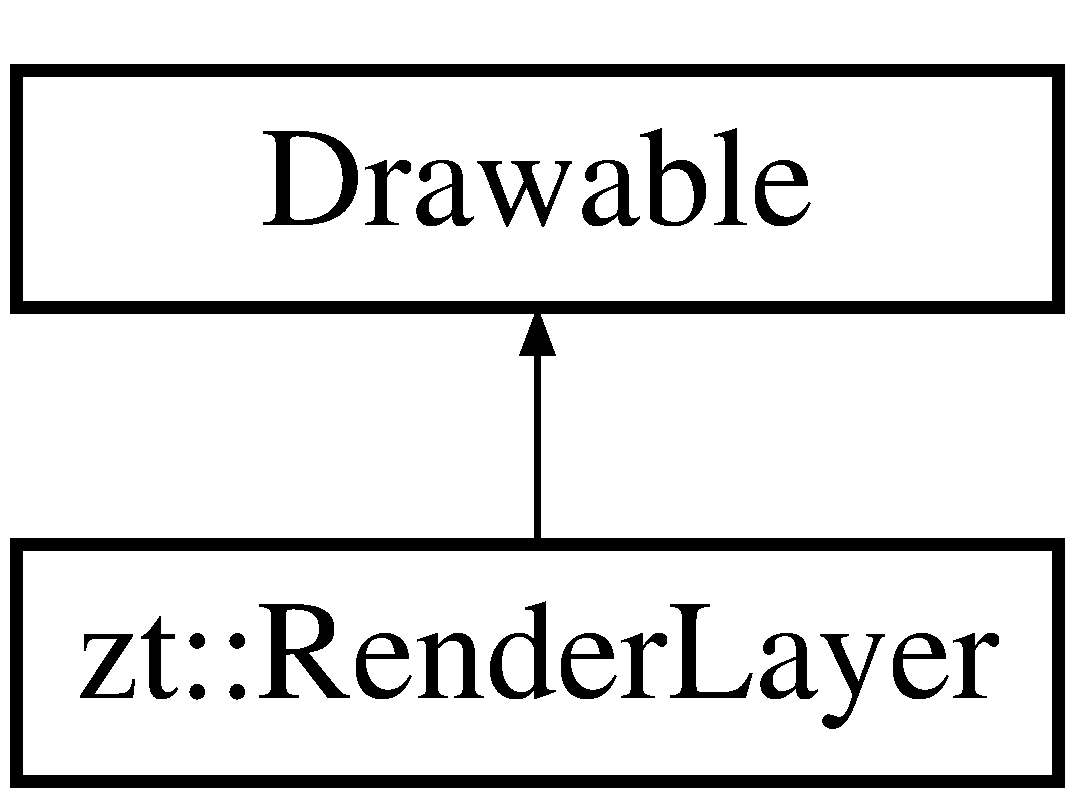
\includegraphics[height=2.000000cm]{classzt_1_1_render_layer}
\end{center}
\end{figure}
\subsection*{Public Member Functions}
\begin{DoxyCompactItemize}
\item 
\mbox{\Hypertarget{classzt_1_1_render_layer_ab612013a9d82ccbe66a7d86b2eb474f2}\label{classzt_1_1_render_layer_ab612013a9d82ccbe66a7d86b2eb474f2}} 
\hyperlink{classzt_1_1_render_layer_ab612013a9d82ccbe66a7d86b2eb474f2}{Render\+Layer} (bool \hyperlink{classzt_1_1_render_layer_a5a6dc2d742807bad7533992512d060b4}{visible}=true)
\begin{DoxyCompactList}\small\item\em Constructs an empty layer. \end{DoxyCompactList}\item 
\mbox{\Hypertarget{classzt_1_1_render_layer_aa1ffedae44104604d9b1ffac7349d181}\label{classzt_1_1_render_layer_aa1ffedae44104604d9b1ffac7349d181}} 
virtual void \hyperlink{classzt_1_1_render_layer_aa1ffedae44104604d9b1ffac7349d181}{draw} (sf\+::\+Render\+Target \&target, sf\+::\+Render\+States states) const
\begin{DoxyCompactList}\small\item\em Draws all contained objects if the layer is visible. \end{DoxyCompactList}\item 
\mbox{\Hypertarget{classzt_1_1_render_layer_a3495a2e7991826fb6459381cd483c96b}\label{classzt_1_1_render_layer_a3495a2e7991826fb6459381cd483c96b}} 
void \hyperlink{classzt_1_1_render_layer_a3495a2e7991826fb6459381cd483c96b}{add\+Drawable} (sf\+::\+Drawable \&item)
\begin{DoxyCompactList}\small\item\em Adds a drawable. \end{DoxyCompactList}\item 
bool \hyperlink{classzt_1_1_render_layer_a7273e706c4f0a727cc363a02b762ebe3}{remove\+Drawable} (sf\+::\+Drawable \&item)
\begin{DoxyCompactList}\small\item\em Removes a drawable if it exists. \end{DoxyCompactList}\item 
\mbox{\Hypertarget{classzt_1_1_render_layer_a93bcd3f29fc6af62bd92ecf670c6368a}\label{classzt_1_1_render_layer_a93bcd3f29fc6af62bd92ecf670c6368a}} 
void \hyperlink{classzt_1_1_render_layer_a93bcd3f29fc6af62bd92ecf670c6368a}{set\+Visible} (bool \hyperlink{classzt_1_1_render_layer_a5a6dc2d742807bad7533992512d060b4}{visible})
\begin{DoxyCompactList}\small\item\em Sets the visibility. \end{DoxyCompactList}\item 
\mbox{\Hypertarget{classzt_1_1_render_layer_a8c7c33d51d373350a5973a55584b394d}\label{classzt_1_1_render_layer_a8c7c33d51d373350a5973a55584b394d}} 
bool {\bfseries is\+Visible} () const
\item 
\mbox{\Hypertarget{classzt_1_1_render_layer_a4a875d392ad3e03acb653f295005909f}\label{classzt_1_1_render_layer_a4a875d392ad3e03acb653f295005909f}} 
int {\bfseries getZ} () const
\item 
\mbox{\Hypertarget{classzt_1_1_render_layer_a112e8fea237b99ab0075a48cc2963b96}\label{classzt_1_1_render_layer_a112e8fea237b99ab0075a48cc2963b96}} 
void {\bfseries setZ} (int z)
\item 
\mbox{\Hypertarget{classzt_1_1_render_layer_a77dc63ee7dc9f16a1d0c2a35beea98f9}\label{classzt_1_1_render_layer_a77dc63ee7dc9f16a1d0c2a35beea98f9}} 
unsigned int {\bfseries count} () const
\item 
\mbox{\Hypertarget{classzt_1_1_render_layer_ad0bbedf8a92173823d16bb7aebedccc6}\label{classzt_1_1_render_layer_ad0bbedf8a92173823d16bb7aebedccc6}} 
bool {\bfseries is\+Empty} () const
\item 
bool \hyperlink{classzt_1_1_render_layer_a7eb4504147aee10b610602c8363311ca}{operator$<$} (\hyperlink{classzt_1_1_render_layer}{zt\+::\+Render\+Layer} \&other) const
\end{DoxyCompactItemize}
\subsection*{Protected Attributes}
\begin{DoxyCompactItemize}
\item 
\mbox{\Hypertarget{classzt_1_1_render_layer_a5a6dc2d742807bad7533992512d060b4}\label{classzt_1_1_render_layer_a5a6dc2d742807bad7533992512d060b4}} 
bool \hyperlink{classzt_1_1_render_layer_a5a6dc2d742807bad7533992512d060b4}{visible}
\begin{DoxyCompactList}\small\item\em If it\textquotesingle{}s false the contained objects won\textquotesingle{}t be drawn. \end{DoxyCompactList}\item 
\mbox{\Hypertarget{classzt_1_1_render_layer_ac19c3e70a9a3329d46b8a16e91aa17e9}\label{classzt_1_1_render_layer_ac19c3e70a9a3329d46b8a16e91aa17e9}} 
std\+::vector$<$ sf\+::\+Drawable $\ast$ $>$ \hyperlink{classzt_1_1_render_layer_ac19c3e70a9a3329d46b8a16e91aa17e9}{drawable\+Items}
\begin{DoxyCompactList}\small\item\em Vector que contiene un puntero a los dibujables de esta capa. \end{DoxyCompactList}\end{DoxyCompactItemize}


\subsection{Detailed Description}
Container for drawable objects. This class allows you to group sf\+::\+Drawable elements such as sf\+::\+Sprite. The container keeps pointers to the objects, so your drawable objects should be kept alive while using the render layer. 

\subsection{Member Function Documentation}
\mbox{\Hypertarget{classzt_1_1_render_layer_a7eb4504147aee10b610602c8363311ca}\label{classzt_1_1_render_layer_a7eb4504147aee10b610602c8363311ca}} 
\index{zt\+::\+Render\+Layer@{zt\+::\+Render\+Layer}!operator$<$@{operator$<$}}
\index{operator$<$@{operator$<$}!zt\+::\+Render\+Layer@{zt\+::\+Render\+Layer}}
\subsubsection{\texorpdfstring{operator$<$()}{operator<()}}
{\footnotesize\ttfamily bool zt\+::\+Render\+Layer\+::operator$<$ (\begin{DoxyParamCaption}\item[{\hyperlink{classzt_1_1_render_layer}{zt\+::\+Render\+Layer} \&}]{other }\end{DoxyParamCaption}) const}

Compares the depth of the layer. 
\begin{DoxyParams}{Parameters}
{\em other} & \\
\hline
\end{DoxyParams}
\begin{DoxyReturn}{Returns}

\end{DoxyReturn}
\mbox{\Hypertarget{classzt_1_1_render_layer_a7273e706c4f0a727cc363a02b762ebe3}\label{classzt_1_1_render_layer_a7273e706c4f0a727cc363a02b762ebe3}} 
\index{zt\+::\+Render\+Layer@{zt\+::\+Render\+Layer}!remove\+Drawable@{remove\+Drawable}}
\index{remove\+Drawable@{remove\+Drawable}!zt\+::\+Render\+Layer@{zt\+::\+Render\+Layer}}
\subsubsection{\texorpdfstring{remove\+Drawable()}{removeDrawable()}}
{\footnotesize\ttfamily bool zt\+::\+Render\+Layer\+::remove\+Drawable (\begin{DoxyParamCaption}\item[{sf\+::\+Drawable \&}]{item }\end{DoxyParamCaption})}



Removes a drawable if it exists. 


\begin{DoxyParams}{Parameters}
{\em item} & Drawable you cant to remove. \\
\hline
\end{DoxyParams}
\begin{DoxyReturn}{Returns}
True if it was removed. 
\end{DoxyReturn}


The documentation for this class was generated from the following file\+:\begin{DoxyCompactItemize}
\item 
include/\+Zelta/\+Core/Render\+Layer.\+hpp\end{DoxyCompactItemize}

\hypertarget{classzt_1_1_resource_manager}{}\section{zt\+:\+:Resource\+Manager$<$ X $>$ Class Template Reference}
\label{classzt_1_1_resource_manager}\index{zt\+::\+Resource\+Manager$<$ X $>$@{zt\+::\+Resource\+Manager$<$ X $>$}}


Base class for resource managers. A resource manager acts as a container for a specific resource type (e.\+g.\+: a sf\+::\+Texture, sf\+::\+Sound\+Buffer).  




{\ttfamily \#include $<$Resource\+Manager.\+hpp$>$}

Inheritance diagram for zt\+:\+:Resource\+Manager$<$ X $>$\+:\begin{figure}[H]
\begin{center}
\leavevmode
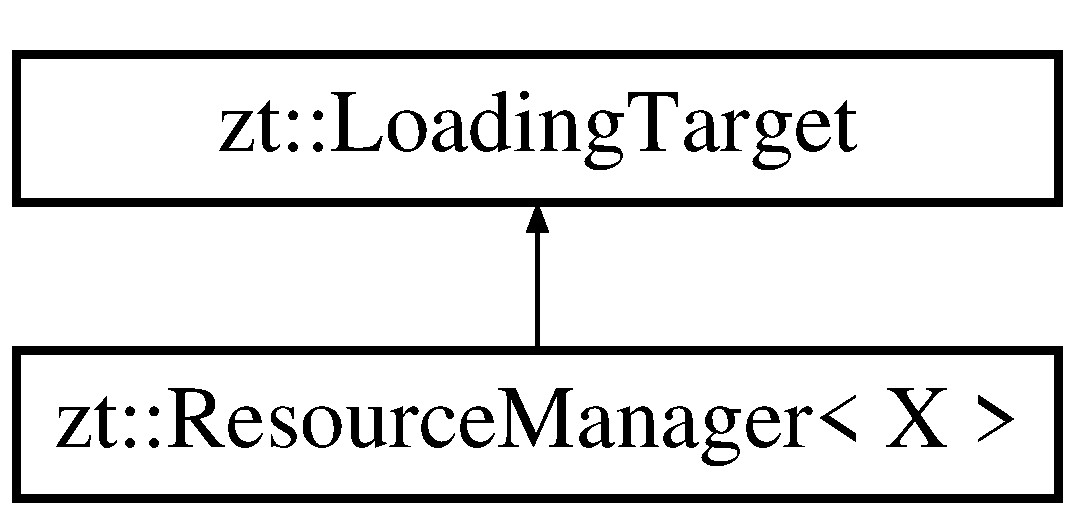
\includegraphics[height=2.000000cm]{classzt_1_1_resource_manager}
\end{center}
\end{figure}
\subsection*{Public Member Functions}
\begin{DoxyCompactItemize}
\item 
\hyperlink{classzt_1_1_resource_manager_aa0973ae6bf2db29a560064101f7e3aa2}{Resource\+Manager} (const std\+::string \&name)
\item 
X \& \hyperlink{classzt_1_1_resource_manager_a5db7d69f549152f521d3e6dc8dceab9d}{get} (const std\+::string \&name)
\item 
X \& \hyperlink{classzt_1_1_resource_manager_a4eeebff68670999944d5a663bbf2c9ed}{operator\mbox{[}$\,$\mbox{]}} (const std\+::string \&name)
\item 
void \hyperlink{classzt_1_1_resource_manager_ad89a189ae9a569688fba24a053e2cd21}{release} (const std\+::string \&name)
\item 
const std\+::string \& \hyperlink{classzt_1_1_resource_manager_a53eff2997bb98a45bce592be5a8cfd89}{get\+Name} () const
\item 
\mbox{\Hypertarget{classzt_1_1_resource_manager_ad9b2235e6ca7136905fc0e9831ca8d19}\label{classzt_1_1_resource_manager_ad9b2235e6ca7136905fc0e9831ca8d19}} 
void {\bfseries pendant} (const std\+::string \&name, \hyperlink{classzt_1_1_resource_provider}{Resource\+Provider} \&provider)
\item 
\mbox{\Hypertarget{classzt_1_1_resource_manager_a52ede9719df15de6396783071b73fed4}\label{classzt_1_1_resource_manager_a52ede9719df15de6396783071b73fed4}} 
void {\bfseries not\+Pendant} (const std\+::string \&name)
\item 
\mbox{\Hypertarget{classzt_1_1_resource_manager_af37584a0c96930f860ea0fc0bfdd11a4}\label{classzt_1_1_resource_manager_af37584a0c96930f860ea0fc0bfdd11a4}} 
bool {\bfseries exists} (const std\+::string \&resource\+Name) const
\item 
\mbox{\Hypertarget{classzt_1_1_resource_manager_a2c4a7986157152012fc7792f9faedf69}\label{classzt_1_1_resource_manager_a2c4a7986157152012fc7792f9faedf69}} 
bool {\bfseries is\+Loaded} (const std\+::string \&resource\+Name) const
\end{DoxyCompactItemize}
\subsection*{Protected Attributes}
\begin{DoxyCompactItemize}
\item 
\mbox{\Hypertarget{classzt_1_1_resource_manager_a78d09009c29b7358e6edf927a82221cf}\label{classzt_1_1_resource_manager_a78d09009c29b7358e6edf927a82221cf}} 
std\+::map$<$ std\+::string, Resource $>$ {\bfseries resources}
\item 
\mbox{\Hypertarget{classzt_1_1_resource_manager_a2bcd33206c69c33054fef8446b78801f}\label{classzt_1_1_resource_manager_a2bcd33206c69c33054fef8446b78801f}} 
std\+::string {\bfseries name}
\end{DoxyCompactItemize}


\subsection{Detailed Description}
\subsubsection*{template$<$class X$>$\newline
class zt\+::\+Resource\+Manager$<$ X $>$}

Base class for resource managers. A resource manager acts as a container for a specific resource type (e.\+g.\+: a sf\+::\+Texture, sf\+::\+Sound\+Buffer). 

\hyperlink{classzt_1_1_resource_manager}{Resource\+Manager} inherits from \hyperlink{classzt_1_1_loading_target}{Loading\+Target}. That means that \hyperlink{classzt_1_1_resource_manager}{Resource\+Manager} is something you can load resources into. All resources in the resource manager are identified by a name that should be unique. You\textquotesingle{}ll request those resources by using that name.

Resources managers also have a unique name which will help the Resource\+Loader to determine to which resource manager load certain resource. 

\subsection{Constructor \& Destructor Documentation}
\mbox{\Hypertarget{classzt_1_1_resource_manager_aa0973ae6bf2db29a560064101f7e3aa2}\label{classzt_1_1_resource_manager_aa0973ae6bf2db29a560064101f7e3aa2}} 
\index{zt\+::\+Resource\+Manager@{zt\+::\+Resource\+Manager}!Resource\+Manager@{Resource\+Manager}}
\index{Resource\+Manager@{Resource\+Manager}!zt\+::\+Resource\+Manager@{zt\+::\+Resource\+Manager}}
\subsubsection{\texorpdfstring{Resource\+Manager()}{ResourceManager()}}
{\footnotesize\ttfamily template$<$class X$>$ \\
\hyperlink{classzt_1_1_resource_manager}{zt\+::\+Resource\+Manager}$<$ X $>$\+::\hyperlink{classzt_1_1_resource_manager}{Resource\+Manager} (\begin{DoxyParamCaption}\item[{const std\+::string \&}]{name }\end{DoxyParamCaption})\hspace{0.3cm}{\ttfamily [inline]}}

Constructs the \hyperlink{classzt_1_1_resource_manager}{Resource\+Manager}. 
\begin{DoxyParams}{Parameters}
{\em name} & Unique name for this \hyperlink{classzt_1_1_resource_manager}{Resource\+Manager}. \\
\hline
\end{DoxyParams}


\subsection{Member Function Documentation}
\mbox{\Hypertarget{classzt_1_1_resource_manager_a5db7d69f549152f521d3e6dc8dceab9d}\label{classzt_1_1_resource_manager_a5db7d69f549152f521d3e6dc8dceab9d}} 
\index{zt\+::\+Resource\+Manager@{zt\+::\+Resource\+Manager}!get@{get}}
\index{get@{get}!zt\+::\+Resource\+Manager@{zt\+::\+Resource\+Manager}}
\subsubsection{\texorpdfstring{get()}{get()}}
{\footnotesize\ttfamily template$<$class X$>$ \\
X\& \hyperlink{classzt_1_1_resource_manager}{zt\+::\+Resource\+Manager}$<$ X $>$\+::get (\begin{DoxyParamCaption}\item[{const std\+::string \&}]{name }\end{DoxyParamCaption})\hspace{0.3cm}{\ttfamily [inline]}}

Get a resource by its name. If the resource is not present it throws a \hyperlink{classzt_1_1_resource_not_found_exception}{Resource\+Not\+Found\+Exception}. 
\begin{DoxyParams}{Parameters}
{\em name} & Name of the resource. \\
\hline
\end{DoxyParams}
\begin{DoxyReturn}{Returns}
Resource. 
\end{DoxyReturn}
\mbox{\Hypertarget{classzt_1_1_resource_manager_a53eff2997bb98a45bce592be5a8cfd89}\label{classzt_1_1_resource_manager_a53eff2997bb98a45bce592be5a8cfd89}} 
\index{zt\+::\+Resource\+Manager@{zt\+::\+Resource\+Manager}!get\+Name@{get\+Name}}
\index{get\+Name@{get\+Name}!zt\+::\+Resource\+Manager@{zt\+::\+Resource\+Manager}}
\subsubsection{\texorpdfstring{get\+Name()}{getName()}}
{\footnotesize\ttfamily template$<$class X$>$ \\
const std\+::string\& \hyperlink{classzt_1_1_resource_manager}{zt\+::\+Resource\+Manager}$<$ X $>$\+::get\+Name (\begin{DoxyParamCaption}{ }\end{DoxyParamCaption}) const\hspace{0.3cm}{\ttfamily [inline]}, {\ttfamily [virtual]}}

Returns the name of this resource manager. \begin{DoxyReturn}{Returns}

\end{DoxyReturn}


Implements \hyperlink{classzt_1_1_loading_target}{zt\+::\+Loading\+Target}.

\mbox{\Hypertarget{classzt_1_1_resource_manager_a4eeebff68670999944d5a663bbf2c9ed}\label{classzt_1_1_resource_manager_a4eeebff68670999944d5a663bbf2c9ed}} 
\index{zt\+::\+Resource\+Manager@{zt\+::\+Resource\+Manager}!operator\mbox{[}\mbox{]}@{operator[]}}
\index{operator\mbox{[}\mbox{]}@{operator[]}!zt\+::\+Resource\+Manager@{zt\+::\+Resource\+Manager}}
\subsubsection{\texorpdfstring{operator[]()}{operator[]()}}
{\footnotesize\ttfamily template$<$class X$>$ \\
X\& \hyperlink{classzt_1_1_resource_manager}{zt\+::\+Resource\+Manager}$<$ X $>$\+::operator\mbox{[}$\,$\mbox{]} (\begin{DoxyParamCaption}\item[{const std\+::string \&}]{name }\end{DoxyParamCaption})\hspace{0.3cm}{\ttfamily [inline]}}

Equivalent to \hyperlink{classzt_1_1_resource_manager_a5db7d69f549152f521d3e6dc8dceab9d}{get()}. \begin{DoxySeeAlso}{See also}
\hyperlink{classzt_1_1_resource_manager_a5db7d69f549152f521d3e6dc8dceab9d}{get()} 
\end{DoxySeeAlso}

\begin{DoxyParams}{Parameters}
{\em name} & Name of the resource. \\
\hline
\end{DoxyParams}
\begin{DoxyReturn}{Returns}
Resource. 
\end{DoxyReturn}
\mbox{\Hypertarget{classzt_1_1_resource_manager_ad89a189ae9a569688fba24a053e2cd21}\label{classzt_1_1_resource_manager_ad89a189ae9a569688fba24a053e2cd21}} 
\index{zt\+::\+Resource\+Manager@{zt\+::\+Resource\+Manager}!release@{release}}
\index{release@{release}!zt\+::\+Resource\+Manager@{zt\+::\+Resource\+Manager}}
\subsubsection{\texorpdfstring{release()}{release()}}
{\footnotesize\ttfamily template$<$class X$>$ \\
void \hyperlink{classzt_1_1_resource_manager}{zt\+::\+Resource\+Manager}$<$ X $>$\+::release (\begin{DoxyParamCaption}\item[{const std\+::string \&}]{name }\end{DoxyParamCaption})\hspace{0.3cm}{\ttfamily [inline]}, {\ttfamily [virtual]}}

Releases a resource. If it does not exist a \hyperlink{classzt_1_1_resource_not_found_exception}{Resource\+Not\+Found\+Exception} is thrown. 
\begin{DoxyParams}{Parameters}
{\em name} & \\
\hline
\end{DoxyParams}


Implements \hyperlink{classzt_1_1_loading_target}{zt\+::\+Loading\+Target}.



The documentation for this class was generated from the following file\+:\begin{DoxyCompactItemize}
\item 
include/\+Zelta/\+Core/Resource\+Manager.\+hpp\end{DoxyCompactItemize}

\hypertarget{classzt_1_1_resource_not_found_exception}{}\section{zt\+:\+:Resource\+Not\+Found\+Exception Class Reference}
\label{classzt_1_1_resource_not_found_exception}\index{zt\+::\+Resource\+Not\+Found\+Exception@{zt\+::\+Resource\+Not\+Found\+Exception}}


Exception throwed when a resource is not found.  




{\ttfamily \#include $<$Resource\+Not\+Found\+Exception.\+hpp$>$}

Inheritance diagram for zt\+:\+:Resource\+Not\+Found\+Exception\+:\begin{figure}[H]
\begin{center}
\leavevmode
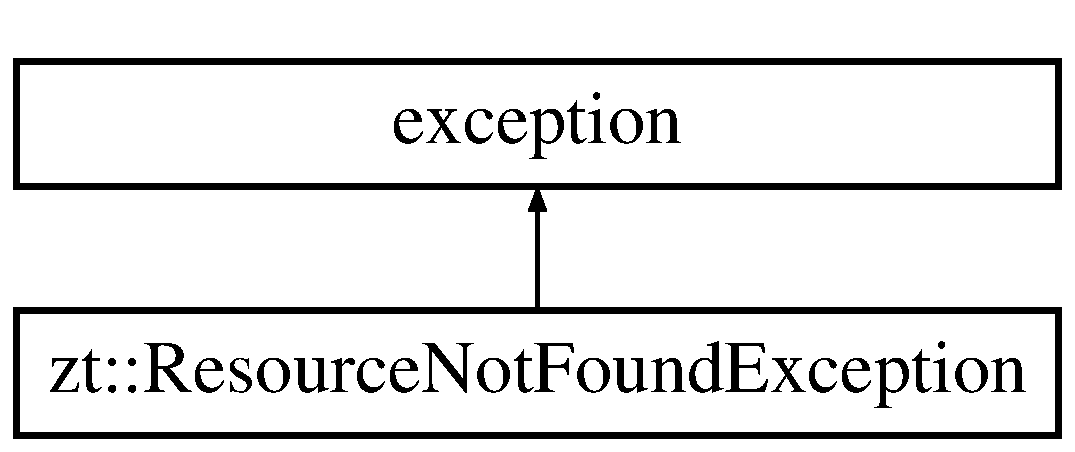
\includegraphics[height=2.000000cm]{classzt_1_1_resource_not_found_exception}
\end{center}
\end{figure}
\subsection*{Public Member Functions}
\begin{DoxyCompactItemize}
\item 
\mbox{\Hypertarget{classzt_1_1_resource_not_found_exception_a3ee4e4b82f9c315f7ab9407905556cc4}\label{classzt_1_1_resource_not_found_exception_a3ee4e4b82f9c315f7ab9407905556cc4}} 
{\bfseries Resource\+Not\+Found\+Exception} (const std\+::string \&resource\+Name)
\item 
\mbox{\Hypertarget{classzt_1_1_resource_not_found_exception_a2cebe772d62daef314041f9ab21d13dd}\label{classzt_1_1_resource_not_found_exception_a2cebe772d62daef314041f9ab21d13dd}} 
const char $\ast$ {\bfseries what} () const noexcept
\end{DoxyCompactItemize}


\subsection{Detailed Description}
Exception throwed when a resource is not found. 

The documentation for this class was generated from the following file\+:\begin{DoxyCompactItemize}
\item 
include/\+Zelta/\+Core/Resource\+Not\+Found\+Exception.\+hpp\end{DoxyCompactItemize}

\hypertarget{classzt_1_1_resource_provider}{}\section{zt\+:\+:Resource\+Provider Class Reference}
\label{classzt_1_1_resource_provider}\index{zt\+::\+Resource\+Provider@{zt\+::\+Resource\+Provider}}


This class allows you to load resources from the filesystem or a package.  




{\ttfamily \#include $<$Resource\+Provider.\+hpp$>$}

\subsection*{Public Member Functions}
\begin{DoxyCompactItemize}
\item 
\mbox{\Hypertarget{classzt_1_1_resource_provider_a377d158f908a51223c9c42f262333ba0}\label{classzt_1_1_resource_provider_a377d158f908a51223c9c42f262333ba0}} 
\hyperlink{classzt_1_1_resource_provider}{Resource\+Provider} \& {\bfseries load} (const std\+::string \&file)
\item 
\mbox{\Hypertarget{classzt_1_1_resource_provider_a4cd1f6c58eef9685bd6ffc761f82168c}\label{classzt_1_1_resource_provider_a4cd1f6c58eef9685bd6ffc761f82168c}} 
\hyperlink{classzt_1_1_resource_provider}{Resource\+Provider} \& {\bfseries from\+File\+System} ()
\item 
\mbox{\Hypertarget{classzt_1_1_resource_provider_aebac197b2ed0b1d95ae366a0732da9ce}\label{classzt_1_1_resource_provider_aebac197b2ed0b1d95ae366a0732da9ce}} 
\hyperlink{classzt_1_1_resource_provider}{Resource\+Provider} \& {\bfseries from\+Package} (const std\+::string \&path)
\item 
\mbox{\Hypertarget{classzt_1_1_resource_provider_aa74e82606ac01a1cc1077fac6a7865ea}\label{classzt_1_1_resource_provider_aa74e82606ac01a1cc1077fac6a7865ea}} 
\hyperlink{classzt_1_1_resource_provider}{Resource\+Provider} \& {\bfseries now} ()
\item 
\mbox{\Hypertarget{classzt_1_1_resource_provider_ac080a462bf92e2d12a4ad15c90e1c182}\label{classzt_1_1_resource_provider_ac080a462bf92e2d12a4ad15c90e1c182}} 
\hyperlink{classzt_1_1_resource_provider}{Resource\+Provider} \& {\bfseries on\+Demand} ()
\item 
\mbox{\Hypertarget{classzt_1_1_resource_provider_aedd409bf8d7bc826d04f8b7750cbd75d}\label{classzt_1_1_resource_provider_aedd409bf8d7bc826d04f8b7750cbd75d}} 
void {\bfseries into} ()
\item 
\mbox{\Hypertarget{classzt_1_1_resource_provider_aa23d6aefb7e5f147b37cf08e3c617b5b}\label{classzt_1_1_resource_provider_aa23d6aefb7e5f147b37cf08e3c617b5b}} 
{\footnotesize template$<$class... TS$>$ }\\void {\bfseries into} (\hyperlink{classzt_1_1_loading_target}{Loading\+Target} \&t, TS \&... ts)
\item 
\mbox{\Hypertarget{classzt_1_1_resource_provider_ac54b02898020c6de5d55698d02383b85}\label{classzt_1_1_resource_provider_ac54b02898020c6de5d55698d02383b85}} 
void {\bfseries require} ()
\item 
{\footnotesize template$<$class S , class... SS$>$ }\\void \hyperlink{classzt_1_1_resource_provider_af7a24c529d5255270e032198c985e603}{require} (S \&t, SS \&...ts)
\begin{DoxyCompactList}\small\item\em This method makes sure that the given resource names are loaded. If they are not, they will be. \end{DoxyCompactList}\item 
\mbox{\Hypertarget{classzt_1_1_resource_provider_aa52dfc3f3022366aa279b78ca36b673e}\label{classzt_1_1_resource_provider_aa52dfc3f3022366aa279b78ca36b673e}} 
void {\bfseries request} (const std\+::string \&type, const std\+::string \&name)
\end{DoxyCompactItemize}
\subsection*{Protected Member Functions}
\begin{DoxyCompactItemize}
\item 
\mbox{\Hypertarget{classzt_1_1_resource_provider_a77afe93ee461dffaa8c1f83b0641d3be}\label{classzt_1_1_resource_provider_a77afe93ee461dffaa8c1f83b0641d3be}} 
void {\bfseries load} (const std\+::string \&type, const std\+::string \&name, const std\+::string \&path)
\item 
bool \hyperlink{classzt_1_1_resource_provider_a40819044cb7a63200d99f73a66887be1}{is\+Loaded} (const std\+::string \&type, const std\+::string \&name)
\begin{DoxyCompactList}\small\item\em This method tells if one resource of certain type is loaded. \end{DoxyCompactList}\end{DoxyCompactItemize}


\subsection{Detailed Description}
This class allows you to load resources from the filesystem or a package. 

The set of resources that will be loaded is determined by a resource file that you set through the load(file) method. (Note\+: that file must not be in a package.) Then you can specify with from\+Filesystem() or from\+Package() where you want to load the resources from. Then you can call the on\+Demand() method, that way the resources will be loaded only when they are requested. Finally, is important to call the into() method to set to which resource managers you will be loading into.

\begin{DoxyWarning}{Warning}
If you are using the on-\/demand loading you must be sure that the \hyperlink{classzt_1_1_resource_provider}{Resource\+Provider} is not destroyed because it will be used by the \hyperlink{classzt_1_1_resource_manager}{Resource\+Manager} to load the requested file. 
\end{DoxyWarning}


\subsection{Member Function Documentation}
\mbox{\Hypertarget{classzt_1_1_resource_provider_a40819044cb7a63200d99f73a66887be1}\label{classzt_1_1_resource_provider_a40819044cb7a63200d99f73a66887be1}} 
\index{zt\+::\+Resource\+Provider@{zt\+::\+Resource\+Provider}!is\+Loaded@{is\+Loaded}}
\index{is\+Loaded@{is\+Loaded}!zt\+::\+Resource\+Provider@{zt\+::\+Resource\+Provider}}
\subsubsection{\texorpdfstring{is\+Loaded()}{isLoaded()}}
{\footnotesize\ttfamily bool zt\+::\+Resource\+Provider\+::is\+Loaded (\begin{DoxyParamCaption}\item[{const std\+::string \&}]{type,  }\item[{const std\+::string \&}]{name }\end{DoxyParamCaption})\hspace{0.3cm}{\ttfamily [inline]}, {\ttfamily [protected]}}



This method tells if one resource of certain type is loaded. 


\begin{DoxyParams}{Parameters}
{\em type} & Type of the resource (the name of the container). \\
\hline
{\em name} & Name of the resource. \\
\hline
\end{DoxyParams}
\begin{DoxyReturn}{Returns}
True if it is loaded. 
\end{DoxyReturn}
\mbox{\Hypertarget{classzt_1_1_resource_provider_af7a24c529d5255270e032198c985e603}\label{classzt_1_1_resource_provider_af7a24c529d5255270e032198c985e603}} 
\index{zt\+::\+Resource\+Provider@{zt\+::\+Resource\+Provider}!require@{require}}
\index{require@{require}!zt\+::\+Resource\+Provider@{zt\+::\+Resource\+Provider}}
\subsubsection{\texorpdfstring{require()}{require()}}
{\footnotesize\ttfamily template$<$class S , class... SS$>$ \\
void zt\+::\+Resource\+Provider\+::require (\begin{DoxyParamCaption}\item[{S \&}]{t,  }\item[{SS \&...}]{ts }\end{DoxyParamCaption})\hspace{0.3cm}{\ttfamily [inline]}}



This method makes sure that the given resource names are loaded. If they are not, they will be. 


\begin{DoxyParams}{Parameters}
{\em t} & Resource name. \\
\hline
{\em ts} & Other resource name. \\
\hline
\end{DoxyParams}


The documentation for this class was generated from the following file\+:\begin{DoxyCompactItemize}
\item 
include/\+Zelta/\+Core/Resource\+Provider.\+hpp\end{DoxyCompactItemize}

\hypertarget{classzt_1_1_scene}{}\section{zt\+:\+:Scene Class Reference}
\label{classzt_1_1_scene}\index{zt\+::\+Scene@{zt\+::\+Scene}}


Represents a game scene. It could be the main menu, the credits scene, etc. This class is made to be inherited from it. Scenes must have a unique name.  




{\ttfamily \#include $<$Scene.\+hpp$>$}

Inheritance diagram for zt\+:\+:Scene\+:\begin{figure}[H]
\begin{center}
\leavevmode
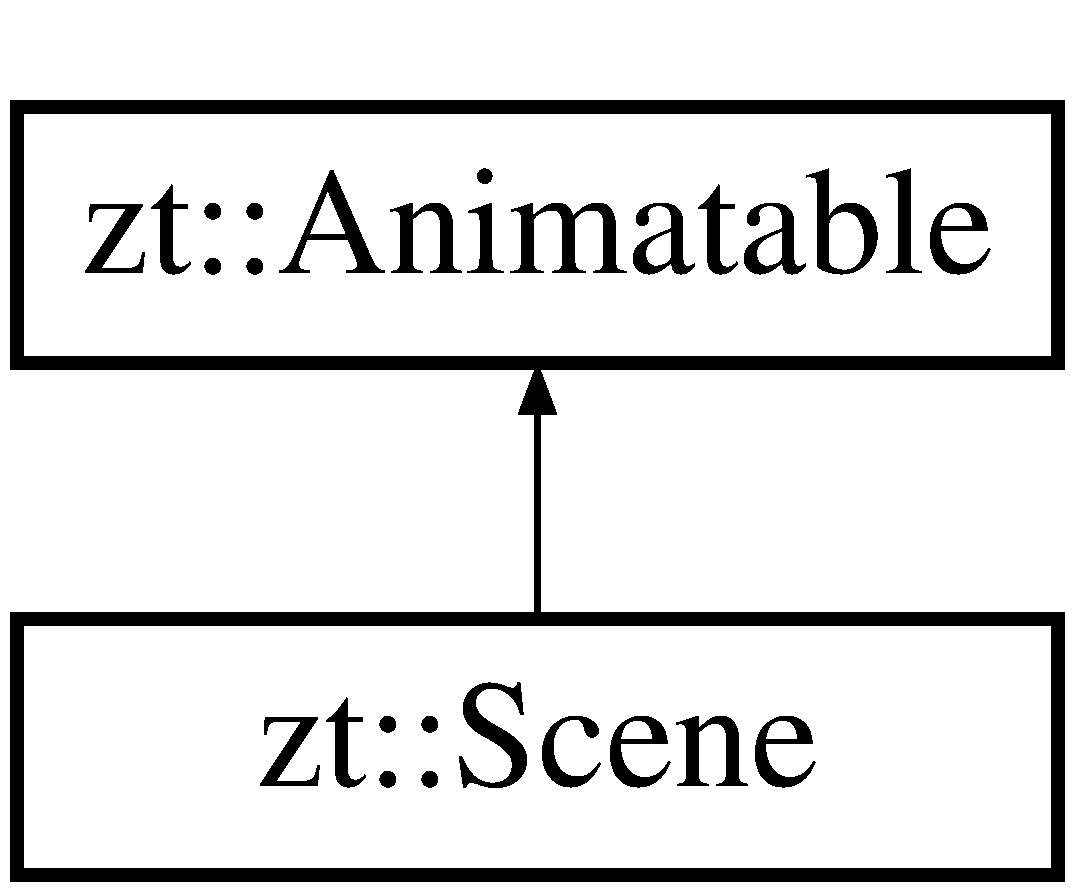
\includegraphics[height=2.000000cm]{classzt_1_1_scene}
\end{center}
\end{figure}
\subsection*{Public Types}
\begin{DoxyCompactItemize}
\item 
\mbox{\Hypertarget{classzt_1_1_scene_a5618d9448cd874af20a6be8ed60c87a5}\label{classzt_1_1_scene_a5618d9448cd874af20a6be8ed60c87a5}} 
enum \hyperlink{classzt_1_1_scene_a5618d9448cd874af20a6be8ed60c87a5}{State} \{ {\bfseries A\+C\+T\+I\+VE}, 
{\bfseries P\+A\+U\+S\+ED}, 
{\bfseries I\+N\+A\+C\+T\+I\+VE}
 \}\begin{DoxyCompactList}\small\item\em States of a scene. \end{DoxyCompactList}
\end{DoxyCompactItemize}
\subsection*{Public Member Functions}
\begin{DoxyCompactItemize}
\item 
\hyperlink{classzt_1_1_scene_af30ef0d6fa9fcdbada43d51f594b1f09}{Scene} (std\+::string name, \hyperlink{classzt_1_1_scene_manager}{Scene\+Manager} \&scene\+Manager)
\begin{DoxyCompactList}\small\item\em Constructs an {\bfseries inactive} scene. \end{DoxyCompactList}\item 
\hyperlink{classzt_1_1_scene_a5618d9448cd874af20a6be8ed60c87a5}{State} \hyperlink{classzt_1_1_scene_a8ee519dcf39f795ebcaf6b3cb2dbb930}{get\+State} () const
\item 
\mbox{\Hypertarget{classzt_1_1_scene_a82fa58fe125a30505c46d94d381e289d}\label{classzt_1_1_scene_a82fa58fe125a30505c46d94d381e289d}} 
std\+::string {\bfseries get\+Name} () const
\item 
virtual void \hyperlink{classzt_1_1_scene_ac7b62a9ada72130fd1d131c080e9a339}{set\+Window} (sf\+::\+Render\+Window \&\hyperlink{classzt_1_1_scene_a03f12b88348262d18487f2381f5874b1}{window})
\begin{DoxyCompactList}\small\item\em Allows you to change the window where you\textquotesingle{}ll be drawing. \end{DoxyCompactList}\item 
\mbox{\Hypertarget{classzt_1_1_scene_a53c482a19ae48fdce5fc3af5e8f3022b}\label{classzt_1_1_scene_a53c482a19ae48fdce5fc3af5e8f3022b}} 
virtual sf\+::\+Render\+Window \& {\bfseries get\+Window} ()
\item 
\mbox{\Hypertarget{classzt_1_1_scene_a571cfe15ea9f8e0b3f1bab35c6d97c6b}\label{classzt_1_1_scene_a571cfe15ea9f8e0b3f1bab35c6d97c6b}} 
virtual sf\+::\+Vector2u {\bfseries get\+Screen\+Size} () const
\item 
\mbox{\Hypertarget{classzt_1_1_scene_adb5f61d68371bdf121766e4bc6116ebe}\label{classzt_1_1_scene_adb5f61d68371bdf121766e4bc6116ebe}} 
virtual \hyperlink{classzt_1_1_nestable_clock}{zt\+::\+Nestable\+Clock} \& {\bfseries get\+Master\+Clock} ()
\item 
\mbox{\Hypertarget{classzt_1_1_scene_a784e245a00b9245faf57d6a6186e8d04}\label{classzt_1_1_scene_a784e245a00b9245faf57d6a6186e8d04}} 
virtual bool {\bfseries is\+Active} () const
\item 
\mbox{\Hypertarget{classzt_1_1_scene_a9ae2b530af478e2444e06c1994531f87}\label{classzt_1_1_scene_a9ae2b530af478e2444e06c1994531f87}} 
virtual bool {\bfseries is\+Inactive} () const
\item 
\mbox{\Hypertarget{classzt_1_1_scene_af2de671d8fa2ef003c0cd55440482464}\label{classzt_1_1_scene_af2de671d8fa2ef003c0cd55440482464}} 
virtual bool {\bfseries is\+Paused} () const
\item 
\mbox{\Hypertarget{classzt_1_1_scene_a7bfc8a6811275f47b858b9baa55ac106}\label{classzt_1_1_scene_a7bfc8a6811275f47b858b9baa55ac106}} 
virtual \hyperlink{classzt_1_1_scene_manager}{Scene\+Manager} \& {\bfseries get\+Scene\+Manager} ()
\end{DoxyCompactItemize}
\subsection*{Protected Member Functions}
\begin{DoxyCompactItemize}
\item 
virtual void \hyperlink{classzt_1_1_scene_a45f434d305b61e9819fb21efe35189dc}{on\+Activate} ()
\begin{DoxyCompactList}\small\item\em This method gets called when the scene is activated. \end{DoxyCompactList}\item 
virtual void \hyperlink{classzt_1_1_scene_a58390d4649c7c0eda1a3fe2f65952a3f}{on\+Deactivate} ()
\begin{DoxyCompactList}\small\item\em This method gets called when the scene is deactivated. \end{DoxyCompactList}\item 
virtual void \hyperlink{classzt_1_1_scene_a38821456606a61abb6255fed9954336e}{on\+Pause} ()
\begin{DoxyCompactList}\small\item\em This method gets called when the scene is paused. \end{DoxyCompactList}\item 
virtual void \hyperlink{classzt_1_1_scene_a0a0d32e948aca8f581a771f54a4444e5}{set\+State} (\hyperlink{classzt_1_1_scene_a5618d9448cd874af20a6be8ed60c87a5}{State} \hyperlink{classzt_1_1_scene_afa7ec29518dcf41daf6e1b33b3241ff8}{state})
\begin{DoxyCompactList}\small\item\em Changes the state of the scene. It\textquotesingle{}s not public because you should change the state of the scene through the scene manager. \end{DoxyCompactList}\item 
virtual void \hyperlink{classzt_1_1_scene_ac5440bbe62a44eda2d4b3d1dde5d3d6a}{advance\+Time} (float delta\+Time)
\begin{DoxyCompactList}\small\item\em This method calls the \hyperlink{classzt_1_1_scene_ac450fd3460c158c0a3f2661df0410477}{manage\+Events()}, \hyperlink{classzt_1_1_scene_a1150eb60893f3077ecacf94b309414bf}{logic()} and \hyperlink{classzt_1_1_scene_aa554c0468228aa1aab7e553c52c7b0d4}{render()} methods. You don\textquotesingle{}t call this method, it\textquotesingle{}s called by the scene manager. \end{DoxyCompactList}\item 
\mbox{\Hypertarget{classzt_1_1_scene_ac450fd3460c158c0a3f2661df0410477}\label{classzt_1_1_scene_ac450fd3460c158c0a3f2661df0410477}} 
virtual void \hyperlink{classzt_1_1_scene_ac450fd3460c158c0a3f2661df0410477}{manage\+Events} (float delta\+Time, std\+::queue$<$ sf\+::\+Event $>$ \&events)
\begin{DoxyCompactList}\small\item\em You should override this method and handle the events from here. \end{DoxyCompactList}\item 
\mbox{\Hypertarget{classzt_1_1_scene_a1150eb60893f3077ecacf94b309414bf}\label{classzt_1_1_scene_a1150eb60893f3077ecacf94b309414bf}} 
virtual void \hyperlink{classzt_1_1_scene_a1150eb60893f3077ecacf94b309414bf}{logic} (float delta\+Time)=0
\begin{DoxyCompactList}\small\item\em You must implement this method. You should handle the logic here. \end{DoxyCompactList}\item 
\mbox{\Hypertarget{classzt_1_1_scene_aa554c0468228aa1aab7e553c52c7b0d4}\label{classzt_1_1_scene_aa554c0468228aa1aab7e553c52c7b0d4}} 
virtual void \hyperlink{classzt_1_1_scene_aa554c0468228aa1aab7e553c52c7b0d4}{render} ()=0
\begin{DoxyCompactList}\small\item\em The drawing stuff goes here. Note that you don\textquotesingle{}t need to call window-\/$>$\hyperlink{classzt_1_1_scene_ae8a778b82813dca9d6153fdcb38896a1}{clear()} nor window-\/$>$display(). The scene manager cares about that. \end{DoxyCompactList}\item 
\mbox{\Hypertarget{classzt_1_1_scene_acfd0b618da5ada48d96b93c8859247af}\label{classzt_1_1_scene_acfd0b618da5ada48d96b93c8859247af}} 
virtual void \hyperlink{classzt_1_1_scene_acfd0b618da5ada48d96b93c8859247af}{check\+If\+Window\+Closed} (sf\+::\+Event event)
\begin{DoxyCompactList}\small\item\em If you call this method inside the poll event loop it will stop all scenes when the window X button is pressed. \end{DoxyCompactList}\item 
\mbox{\Hypertarget{classzt_1_1_scene_ac0fa65322c3b81f42b2386d14e55e14f}\label{classzt_1_1_scene_ac0fa65322c3b81f42b2386d14e55e14f}} 
virtual void \hyperlink{classzt_1_1_scene_ac0fa65322c3b81f42b2386d14e55e14f}{draw} (const sf\+::\+Drawable \&drawable) const
\begin{DoxyCompactList}\small\item\em Helper method to draw things easily. Instead of calling window-\/$>$draw(something) you just need to call draw(something). \end{DoxyCompactList}\item 
virtual void \hyperlink{classzt_1_1_scene_ae8a778b82813dca9d6153fdcb38896a1}{clear} (const sf\+::\+Color \&color=sf\+::\+Color\+::\+Black)
\begin{DoxyCompactList}\small\item\em Clears the screen. \end{DoxyCompactList}\end{DoxyCompactItemize}
\subsection*{Protected Attributes}
\begin{DoxyCompactItemize}
\item 
\mbox{\Hypertarget{classzt_1_1_scene_a2a64a5a0a5c38c79416f1887ad8ddf1d}\label{classzt_1_1_scene_a2a64a5a0a5c38c79416f1887ad8ddf1d}} 
\hyperlink{classzt_1_1_scene_manager}{Scene\+Manager} $\ast$ {\bfseries scene\+Manager}
\item 
\mbox{\Hypertarget{classzt_1_1_scene_afa7ec29518dcf41daf6e1b33b3241ff8}\label{classzt_1_1_scene_afa7ec29518dcf41daf6e1b33b3241ff8}} 
\hyperlink{classzt_1_1_scene_a5618d9448cd874af20a6be8ed60c87a5}{State} \hyperlink{classzt_1_1_scene_afa7ec29518dcf41daf6e1b33b3241ff8}{state}
\begin{DoxyCompactList}\small\item\em Current state. \end{DoxyCompactList}\item 
\mbox{\Hypertarget{classzt_1_1_scene_a03f12b88348262d18487f2381f5874b1}\label{classzt_1_1_scene_a03f12b88348262d18487f2381f5874b1}} 
sf\+::\+Render\+Window $\ast$ \hyperlink{classzt_1_1_scene_a03f12b88348262d18487f2381f5874b1}{window}
\begin{DoxyCompactList}\small\item\em Pointer to the current window. \end{DoxyCompactList}\item 
\mbox{\Hypertarget{classzt_1_1_scene_a4c59d38b4006405c0f5a4caae401500e}\label{classzt_1_1_scene_a4c59d38b4006405c0f5a4caae401500e}} 
std\+::string {\bfseries name}
\item 
\mbox{\Hypertarget{classzt_1_1_scene_a1da96e1c8fa7b26da4504ade1bfd6c41}\label{classzt_1_1_scene_a1da96e1c8fa7b26da4504ade1bfd6c41}} 
std\+::queue$<$ sf\+::\+Event $>$ {\bfseries events}
\item 
\mbox{\Hypertarget{classzt_1_1_scene_a4cc8f5e29b99c49a8edc0c8a2f535d3c}\label{classzt_1_1_scene_a4cc8f5e29b99c49a8edc0c8a2f535d3c}} 
\hyperlink{classzt_1_1_nestable_clock}{zt\+::\+Nestable\+Clock} {\bfseries master\+Clock}
\end{DoxyCompactItemize}
\subsection*{Friends}
\begin{DoxyCompactItemize}
\item 
\mbox{\Hypertarget{classzt_1_1_scene_a284464b0561a6f2915f04b0245b987f0}\label{classzt_1_1_scene_a284464b0561a6f2915f04b0245b987f0}} 
class {\bfseries Scene\+Manager}
\end{DoxyCompactItemize}


\subsection{Detailed Description}
Represents a game scene. It could be the main menu, the credits scene, etc. This class is made to be inherited from it. Scenes must have a unique name. 

There are three methods you\textquotesingle{}ll want/have to override\+: -\/manage\+Events()\+: this is the place to manage the events. The current behaviour of this method is to finish the game when you click the X button. -\/logic()\+: you can place the logic here. -\/draw()\+: rendering stuff goes here.

The \hyperlink{classzt_1_1_scene}{Scene} class does not really care about where you put your logic or your event handling. That means that you can put your logic in the \hyperlink{classzt_1_1_scene_ac450fd3460c158c0a3f2661df0410477}{manage\+Events()} method and handle the events in the \hyperlink{classzt_1_1_scene_a1150eb60893f3077ecacf94b309414bf}{logic()} one. Of course, you shouldn\textquotesingle{}t.

Both \hyperlink{classzt_1_1_scene_ac450fd3460c158c0a3f2661df0410477}{manage\+Events()} and \hyperlink{classzt_1_1_scene_a1150eb60893f3077ecacf94b309414bf}{logic()} receive the delta\+Time as argument to move things accordingly with the frame rate, \hyperlink{classzt_1_1_scene_aa554c0468228aa1aab7e553c52c7b0d4}{render()} doesn\textquotesingle{}t because you should not update anything there.

Sometimes the order in which these methods are called is important. By default, they are called like this\+: \hyperlink{classzt_1_1_scene_ac450fd3460c158c0a3f2661df0410477}{manage\+Events()} then \hyperlink{classzt_1_1_scene_a1150eb60893f3077ecacf94b309414bf}{logic()} then \hyperlink{classzt_1_1_scene_aa554c0468228aa1aab7e553c52c7b0d4}{render()}. You can change this behaviour by overriding the \hyperlink{classzt_1_1_scene_ac5440bbe62a44eda2d4b3d1dde5d3d6a}{advance\+Time()} method.

Keep in mind that the \hyperlink{classzt_1_1_scene_ac5440bbe62a44eda2d4b3d1dde5d3d6a}{advance\+Time()} method is called from the game loop, but this method {\bfseries is not} the game loop. The game loop is in the scene manager. 

\subsection{Constructor \& Destructor Documentation}
\mbox{\Hypertarget{classzt_1_1_scene_af30ef0d6fa9fcdbada43d51f594b1f09}\label{classzt_1_1_scene_af30ef0d6fa9fcdbada43d51f594b1f09}} 
\index{zt\+::\+Scene@{zt\+::\+Scene}!Scene@{Scene}}
\index{Scene@{Scene}!zt\+::\+Scene@{zt\+::\+Scene}}
\subsubsection{\texorpdfstring{Scene()}{Scene()}}
{\footnotesize\ttfamily zt\+::\+Scene\+::\+Scene (\begin{DoxyParamCaption}\item[{std\+::string}]{name,  }\item[{\hyperlink{classzt_1_1_scene_manager}{Scene\+Manager} \&}]{scene\+Manager }\end{DoxyParamCaption})}



Constructs an {\bfseries inactive} scene. 


\begin{DoxyParams}{Parameters}
{\em name} & Unique name for the scene. \\
\hline
{\em window} & Reference to the window where you\textquotesingle{}ll draw your stuff. \\
\hline
\end{DoxyParams}


\subsection{Member Function Documentation}
\mbox{\Hypertarget{classzt_1_1_scene_ac5440bbe62a44eda2d4b3d1dde5d3d6a}\label{classzt_1_1_scene_ac5440bbe62a44eda2d4b3d1dde5d3d6a}} 
\index{zt\+::\+Scene@{zt\+::\+Scene}!advance\+Time@{advance\+Time}}
\index{advance\+Time@{advance\+Time}!zt\+::\+Scene@{zt\+::\+Scene}}
\subsubsection{\texorpdfstring{advance\+Time()}{advanceTime()}}
{\footnotesize\ttfamily virtual void zt\+::\+Scene\+::advance\+Time (\begin{DoxyParamCaption}\item[{float}]{delta\+Time }\end{DoxyParamCaption})\hspace{0.3cm}{\ttfamily [protected]}, {\ttfamily [virtual]}}



This method calls the \hyperlink{classzt_1_1_scene_ac450fd3460c158c0a3f2661df0410477}{manage\+Events()}, \hyperlink{classzt_1_1_scene_a1150eb60893f3077ecacf94b309414bf}{logic()} and \hyperlink{classzt_1_1_scene_aa554c0468228aa1aab7e553c52c7b0d4}{render()} methods. You don\textquotesingle{}t call this method, it\textquotesingle{}s called by the scene manager. 

By default, \hyperlink{classzt_1_1_scene_ac450fd3460c158c0a3f2661df0410477}{manage\+Events()} and \hyperlink{classzt_1_1_scene_a1150eb60893f3077ecacf94b309414bf}{logic()} are only called when the scene is active. The \hyperlink{classzt_1_1_scene_aa554c0468228aa1aab7e553c52c7b0d4}{render()} method is also called when the scene is paused. You may want to override this behaviour. 
\begin{DoxyParams}{Parameters}
{\em delta\+Time} & \\
\hline
\end{DoxyParams}


Implements \hyperlink{classzt_1_1_animatable}{zt\+::\+Animatable}.

\mbox{\Hypertarget{classzt_1_1_scene_ae8a778b82813dca9d6153fdcb38896a1}\label{classzt_1_1_scene_ae8a778b82813dca9d6153fdcb38896a1}} 
\index{zt\+::\+Scene@{zt\+::\+Scene}!clear@{clear}}
\index{clear@{clear}!zt\+::\+Scene@{zt\+::\+Scene}}
\subsubsection{\texorpdfstring{clear()}{clear()}}
{\footnotesize\ttfamily virtual void zt\+::\+Scene\+::clear (\begin{DoxyParamCaption}\item[{const sf\+::\+Color \&}]{color = {\ttfamily sf\+:\+:Color\+:\+:Black} }\end{DoxyParamCaption})\hspace{0.3cm}{\ttfamily [protected]}, {\ttfamily [virtual]}}



Clears the screen. 


\begin{DoxyParams}{Parameters}
{\em color} & \\
\hline
\end{DoxyParams}
\mbox{\Hypertarget{classzt_1_1_scene_a8ee519dcf39f795ebcaf6b3cb2dbb930}\label{classzt_1_1_scene_a8ee519dcf39f795ebcaf6b3cb2dbb930}} 
\index{zt\+::\+Scene@{zt\+::\+Scene}!get\+State@{get\+State}}
\index{get\+State@{get\+State}!zt\+::\+Scene@{zt\+::\+Scene}}
\subsubsection{\texorpdfstring{get\+State()}{getState()}}
{\footnotesize\ttfamily \hyperlink{classzt_1_1_scene_a5618d9448cd874af20a6be8ed60c87a5}{State} zt\+::\+Scene\+::get\+State (\begin{DoxyParamCaption}{ }\end{DoxyParamCaption}) const}

\begin{DoxyReturn}{Returns}
Current state. 
\end{DoxyReturn}
\begin{DoxySeeAlso}{See also}
\hyperlink{classzt_1_1_scene_a5618d9448cd874af20a6be8ed60c87a5}{State} 
\end{DoxySeeAlso}
\mbox{\Hypertarget{classzt_1_1_scene_a45f434d305b61e9819fb21efe35189dc}\label{classzt_1_1_scene_a45f434d305b61e9819fb21efe35189dc}} 
\index{zt\+::\+Scene@{zt\+::\+Scene}!on\+Activate@{on\+Activate}}
\index{on\+Activate@{on\+Activate}!zt\+::\+Scene@{zt\+::\+Scene}}
\subsubsection{\texorpdfstring{on\+Activate()}{onActivate()}}
{\footnotesize\ttfamily virtual void zt\+::\+Scene\+::on\+Activate (\begin{DoxyParamCaption}{ }\end{DoxyParamCaption})\hspace{0.3cm}{\ttfamily [protected]}, {\ttfamily [virtual]}}



This method gets called when the scene is activated. 

\begin{DoxyNote}{Note}
If you override this method do not forget to call the parent \hyperlink{classzt_1_1_scene_a45f434d305b61e9819fb21efe35189dc}{on\+Activate()} method or it will not be activated. 
\end{DoxyNote}
\mbox{\Hypertarget{classzt_1_1_scene_a58390d4649c7c0eda1a3fe2f65952a3f}\label{classzt_1_1_scene_a58390d4649c7c0eda1a3fe2f65952a3f}} 
\index{zt\+::\+Scene@{zt\+::\+Scene}!on\+Deactivate@{on\+Deactivate}}
\index{on\+Deactivate@{on\+Deactivate}!zt\+::\+Scene@{zt\+::\+Scene}}
\subsubsection{\texorpdfstring{on\+Deactivate()}{onDeactivate()}}
{\footnotesize\ttfamily virtual void zt\+::\+Scene\+::on\+Deactivate (\begin{DoxyParamCaption}{ }\end{DoxyParamCaption})\hspace{0.3cm}{\ttfamily [protected]}, {\ttfamily [virtual]}}



This method gets called when the scene is deactivated. 

\begin{DoxyNote}{Note}
If you override this method do not forget to call the parent on\+Deactivated() method or it will not be activated. 
\end{DoxyNote}
\mbox{\Hypertarget{classzt_1_1_scene_a38821456606a61abb6255fed9954336e}\label{classzt_1_1_scene_a38821456606a61abb6255fed9954336e}} 
\index{zt\+::\+Scene@{zt\+::\+Scene}!on\+Pause@{on\+Pause}}
\index{on\+Pause@{on\+Pause}!zt\+::\+Scene@{zt\+::\+Scene}}
\subsubsection{\texorpdfstring{on\+Pause()}{onPause()}}
{\footnotesize\ttfamily virtual void zt\+::\+Scene\+::on\+Pause (\begin{DoxyParamCaption}{ }\end{DoxyParamCaption})\hspace{0.3cm}{\ttfamily [protected]}, {\ttfamily [virtual]}}



This method gets called when the scene is paused. 

\begin{DoxyNote}{Note}
If you override this method do not forget to call the parent on\+Paused() method or it will not be activated. 
\end{DoxyNote}
\mbox{\Hypertarget{classzt_1_1_scene_a0a0d32e948aca8f581a771f54a4444e5}\label{classzt_1_1_scene_a0a0d32e948aca8f581a771f54a4444e5}} 
\index{zt\+::\+Scene@{zt\+::\+Scene}!set\+State@{set\+State}}
\index{set\+State@{set\+State}!zt\+::\+Scene@{zt\+::\+Scene}}
\subsubsection{\texorpdfstring{set\+State()}{setState()}}
{\footnotesize\ttfamily virtual void zt\+::\+Scene\+::set\+State (\begin{DoxyParamCaption}\item[{\hyperlink{classzt_1_1_scene_a5618d9448cd874af20a6be8ed60c87a5}{State}}]{state }\end{DoxyParamCaption})\hspace{0.3cm}{\ttfamily [protected]}, {\ttfamily [virtual]}}



Changes the state of the scene. It\textquotesingle{}s not public because you should change the state of the scene through the scene manager. 


\begin{DoxyParams}{Parameters}
{\em state} & New state. \\
\hline
\end{DoxyParams}
\mbox{\Hypertarget{classzt_1_1_scene_ac7b62a9ada72130fd1d131c080e9a339}\label{classzt_1_1_scene_ac7b62a9ada72130fd1d131c080e9a339}} 
\index{zt\+::\+Scene@{zt\+::\+Scene}!set\+Window@{set\+Window}}
\index{set\+Window@{set\+Window}!zt\+::\+Scene@{zt\+::\+Scene}}
\subsubsection{\texorpdfstring{set\+Window()}{setWindow()}}
{\footnotesize\ttfamily virtual void zt\+::\+Scene\+::set\+Window (\begin{DoxyParamCaption}\item[{sf\+::\+Render\+Window \&}]{window }\end{DoxyParamCaption})\hspace{0.3cm}{\ttfamily [virtual]}}



Allows you to change the window where you\textquotesingle{}ll be drawing. 


\begin{DoxyParams}{Parameters}
{\em window} & Window. \\
\hline
\end{DoxyParams}


The documentation for this class was generated from the following file\+:\begin{DoxyCompactItemize}
\item 
include/\+Zelta/\+Core/Scene.\+hpp\end{DoxyCompactItemize}

\hypertarget{classzt_1_1_scene_manager}{}\section{zt\+:\+:Scene\+Manager Class Reference}
\label{classzt_1_1_scene_manager}\index{zt\+::\+Scene\+Manager@{zt\+::\+Scene\+Manager}}


This class manages scenes. Scenes added to the scene manager must have a unique name. You\textquotesingle{}ll activate them through the \hyperlink{classzt_1_1_scene_manager}{Scene\+Manager}.  




{\ttfamily \#include $<$Scene\+Manager.\+hpp$>$}

\subsection*{Public Member Functions}
\begin{DoxyCompactItemize}
\item 
\mbox{\Hypertarget{classzt_1_1_scene_manager_af087c4fb01189e095d9221efb54619dc}\label{classzt_1_1_scene_manager_af087c4fb01189e095d9221efb54619dc}} 
{\bfseries Scene\+Manager} (sf\+::\+Render\+Window \&window)
\item 
void \hyperlink{classzt_1_1_scene_manager_ad6bee2cb8d320e788a2eda8fcdebdbc9}{set\+Render\+Window} (sf\+::\+Render\+Window \&\hyperlink{classzt_1_1_scene_manager_a1a0c6b40321c66709ae36f3ccd9f84f6}{render\+Window})
\begin{DoxyCompactList}\small\item\em Sets the window. \end{DoxyCompactList}\item 
void \hyperlink{classzt_1_1_scene_manager_a063202765a5b757eae0d28bb9badc53b}{add\+Scene} (\hyperlink{classzt_1_1_scene}{zt\+::\+Scene} \&scene)
\begin{DoxyCompactList}\small\item\em Adds a \hyperlink{classzt_1_1_scene}{Scene}. \end{DoxyCompactList}\item 
\mbox{\Hypertarget{classzt_1_1_scene_manager_a9385d452cd66294db0c03b6366519d4a}\label{classzt_1_1_scene_manager_a9385d452cd66294db0c03b6366519d4a}} 
void \hyperlink{classzt_1_1_scene_manager_a9385d452cd66294db0c03b6366519d4a}{manage} ()
\begin{DoxyCompactList}\small\item\em This is the actual game loop. This function will return when all scenes are inactive. \end{DoxyCompactList}\item 
void \hyperlink{classzt_1_1_scene_manager_acee2eb38afb510f701dc3dd3c5fe3482}{activate\+Scene} (std\+::string name)
\begin{DoxyCompactList}\small\item\em Activates a \hyperlink{classzt_1_1_scene}{Scene}. \end{DoxyCompactList}\item 
void \hyperlink{classzt_1_1_scene_manager_a90a6e2b62f58123056dd3d475cb64165}{switch\+To} (std\+::string name)
\begin{DoxyCompactList}\small\item\em Activate a scene and deactivate the others. \end{DoxyCompactList}\item 
void \hyperlink{classzt_1_1_scene_manager_a6adb888b88566305c08f1b57b33dbb83}{deactivate\+Scene} (std\+::string name)
\begin{DoxyCompactList}\small\item\em Deactivate a scene. \end{DoxyCompactList}\item 
\mbox{\Hypertarget{classzt_1_1_scene_manager_a6afb9d6bd8ff0b537d55128fbd9be96a}\label{classzt_1_1_scene_manager_a6afb9d6bd8ff0b537d55128fbd9be96a}} 
void \hyperlink{classzt_1_1_scene_manager_a6afb9d6bd8ff0b537d55128fbd9be96a}{deactivate\+All\+Scenes} ()
\begin{DoxyCompactList}\small\item\em Deactivates all scenes, thus, the game loop will finish. \end{DoxyCompactList}\item 
void \hyperlink{classzt_1_1_scene_manager_ac8864d3586a8fa7ce01a7c5c007dd5e7}{pause\+Scene} (std\+::string name)
\begin{DoxyCompactList}\small\item\em Pauses the scene. \end{DoxyCompactList}\item 
\mbox{\Hypertarget{classzt_1_1_scene_manager_a5e7367b8f8bc358a974220e9ae58ab0a}\label{classzt_1_1_scene_manager_a5e7367b8f8bc358a974220e9ae58ab0a}} 
void \hyperlink{classzt_1_1_scene_manager_a5e7367b8f8bc358a974220e9ae58ab0a}{remove\+Scene} (std\+::string name)
\begin{DoxyCompactList}\small\item\em Removes a scene. \end{DoxyCompactList}\item 
bool \hyperlink{classzt_1_1_scene_manager_a9b84c499ed47c2f58ef6e7ea8edba296}{all\+Scenes\+Inactive} () const
\item 
\mbox{\Hypertarget{classzt_1_1_scene_manager_a3a0edba9daf3e9fe063b621dc39310c9}\label{classzt_1_1_scene_manager_a3a0edba9daf3e9fe063b621dc39310c9}} 
sf\+::\+Render\+Window \& {\bfseries get\+Render\+Window} ()
\item 
\mbox{\Hypertarget{classzt_1_1_scene_manager_a44481a7e109706c111c38c985d9caedb}\label{classzt_1_1_scene_manager_a44481a7e109706c111c38c985d9caedb}} 
void {\bfseries move\+Forward} (const std\+::string \&scene\+Name)
\item 
\mbox{\Hypertarget{classzt_1_1_scene_manager_aeed45624540e6b59e5ae0f78468b4f29}\label{classzt_1_1_scene_manager_aeed45624540e6b59e5ae0f78468b4f29}} 
void {\bfseries move\+To\+Front} (const std\+::string \&scene\+Name)
\item 
\mbox{\Hypertarget{classzt_1_1_scene_manager_a8caa94629a100ae3db366b10f76f7c54}\label{classzt_1_1_scene_manager_a8caa94629a100ae3db366b10f76f7c54}} 
void {\bfseries move\+Backward} (const std\+::string \&scene\+Name)
\item 
\mbox{\Hypertarget{classzt_1_1_scene_manager_acb09572788f74b46f0c445c5b47b9489}\label{classzt_1_1_scene_manager_acb09572788f74b46f0c445c5b47b9489}} 
void {\bfseries move\+To\+Back} (const std\+::string \&scene\+Name)
\item 
\mbox{\Hypertarget{classzt_1_1_scene_manager_a4aa593d96a651a6512da4d1c4a53b345}\label{classzt_1_1_scene_manager_a4aa593d96a651a6512da4d1c4a53b345}} 
void {\bfseries set\+Scenes\+Order} ()
\item 
\mbox{\Hypertarget{classzt_1_1_scene_manager_a16dcc1decc831c9eeef7910c4ed87e02}\label{classzt_1_1_scene_manager_a16dcc1decc831c9eeef7910c4ed87e02}} 
{\footnotesize template$<$typename... TS$>$ }\\void {\bfseries set\+Scenes\+Order} (T\+S... others, const std\+::string \&name)
\end{DoxyCompactItemize}
\subsection*{Protected Member Functions}
\begin{DoxyCompactItemize}
\item 
\mbox{\Hypertarget{classzt_1_1_scene_manager_a4390bf866b30292dbf27eae3f56bfa31}\label{classzt_1_1_scene_manager_a4390bf866b30292dbf27eae3f56bfa31}} 
void \hyperlink{classzt_1_1_scene_manager_a4390bf866b30292dbf27eae3f56bfa31}{start\+Render} ()
\begin{DoxyCompactList}\small\item\em This method is called just before the all render() methods from scenes are called. It clears the screen. \end{DoxyCompactList}\item 
\mbox{\Hypertarget{classzt_1_1_scene_manager_a66015a7d3051185c09a03ad184101b89}\label{classzt_1_1_scene_manager_a66015a7d3051185c09a03ad184101b89}} 
void \hyperlink{classzt_1_1_scene_manager_a66015a7d3051185c09a03ad184101b89}{stop\+Render} ()
\begin{DoxyCompactList}\small\item\em This method is called just after all render() methods from scenes are called. It displays the drawed stuff. \end{DoxyCompactList}\item 
\hyperlink{classzt_1_1_scene}{Scene} $\ast$ \hyperlink{classzt_1_1_scene_manager_a8587fc624ef29ac0d71ff72a8a653066}{look\+For\+Scene} (std\+::string name)
\end{DoxyCompactItemize}
\subsection*{Protected Attributes}
\begin{DoxyCompactItemize}
\item 
\mbox{\Hypertarget{classzt_1_1_scene_manager_a1a0c6b40321c66709ae36f3ccd9f84f6}\label{classzt_1_1_scene_manager_a1a0c6b40321c66709ae36f3ccd9f84f6}} 
sf\+::\+Render\+Window $\ast$ \hyperlink{classzt_1_1_scene_manager_a1a0c6b40321c66709ae36f3ccd9f84f6}{render\+Window}
\begin{DoxyCompactList}\small\item\em Pointer to the window. The \hyperlink{classzt_1_1_scene_manager}{Scene\+Manager} frees you from having to call window-\/$>$clear() and window-\/$>$display() from your scenes. \end{DoxyCompactList}\item 
\mbox{\Hypertarget{classzt_1_1_scene_manager_ae79370ebeb570c32b61f2d99f443762f}\label{classzt_1_1_scene_manager_ae79370ebeb570c32b61f2d99f443762f}} 
std\+::list$<$ \hyperlink{classzt_1_1_scene}{Scene} $\ast$ $>$ {\bfseries scenes}
\item 
\mbox{\Hypertarget{classzt_1_1_scene_manager_a4b874be56a77810968973b7c6c5e850a}\label{classzt_1_1_scene_manager_a4b874be56a77810968973b7c6c5e850a}} 
sf\+::\+Clock \hyperlink{classzt_1_1_scene_manager_a4b874be56a77810968973b7c6c5e850a}{delta\+Time}
\begin{DoxyCompactList}\small\item\em This clock is used to calc the delta time. All scenes get this information from the \hyperlink{classzt_1_1_scene_manager}{Scene\+Manager} and use that number to move things accordingly with it. \end{DoxyCompactList}\item 
\mbox{\Hypertarget{classzt_1_1_scene_manager_ab98ec372db998caa20e060a6e49fed72}\label{classzt_1_1_scene_manager_ab98ec372db998caa20e060a6e49fed72}} 
std\+::deque$<$ sf\+::\+Event $>$ \hyperlink{classzt_1_1_scene_manager_ab98ec372db998caa20e060a6e49fed72}{events}
\begin{DoxyCompactList}\small\item\em Stores the event queue from the window. We store it because we\textquotesingle{}ll be giving a copy of the queue to each scene so that all of them can handle the events. \end{DoxyCompactList}\end{DoxyCompactItemize}


\subsection{Detailed Description}
This class manages scenes. Scenes added to the scene manager must have a unique name. You\textquotesingle{}ll activate them through the \hyperlink{classzt_1_1_scene_manager}{Scene\+Manager}. 

The \hyperlink{classzt_1_1_scene_manager_a9385d452cd66294db0c03b6366519d4a}{manage()} method contains the main loop which will call the manage\+Events(), logic() and render() methods of your scenes. 

\subsection{Member Function Documentation}
\mbox{\Hypertarget{classzt_1_1_scene_manager_acee2eb38afb510f701dc3dd3c5fe3482}\label{classzt_1_1_scene_manager_acee2eb38afb510f701dc3dd3c5fe3482}} 
\index{zt\+::\+Scene\+Manager@{zt\+::\+Scene\+Manager}!activate\+Scene@{activate\+Scene}}
\index{activate\+Scene@{activate\+Scene}!zt\+::\+Scene\+Manager@{zt\+::\+Scene\+Manager}}
\subsubsection{\texorpdfstring{activate\+Scene()}{activateScene()}}
{\footnotesize\ttfamily void zt\+::\+Scene\+Manager\+::activate\+Scene (\begin{DoxyParamCaption}\item[{std\+::string}]{name }\end{DoxyParamCaption})}



Activates a \hyperlink{classzt_1_1_scene}{Scene}. 


\begin{DoxyParams}{Parameters}
{\em name} & Name of the scene. \\
\hline
\end{DoxyParams}
\mbox{\Hypertarget{classzt_1_1_scene_manager_a063202765a5b757eae0d28bb9badc53b}\label{classzt_1_1_scene_manager_a063202765a5b757eae0d28bb9badc53b}} 
\index{zt\+::\+Scene\+Manager@{zt\+::\+Scene\+Manager}!add\+Scene@{add\+Scene}}
\index{add\+Scene@{add\+Scene}!zt\+::\+Scene\+Manager@{zt\+::\+Scene\+Manager}}
\subsubsection{\texorpdfstring{add\+Scene()}{addScene()}}
{\footnotesize\ttfamily void zt\+::\+Scene\+Manager\+::add\+Scene (\begin{DoxyParamCaption}\item[{\hyperlink{classzt_1_1_scene}{zt\+::\+Scene} \&}]{scene }\end{DoxyParamCaption})}



Adds a \hyperlink{classzt_1_1_scene}{Scene}. 


\begin{DoxyParams}{Parameters}
{\em scene} & \hyperlink{classzt_1_1_scene}{Scene}. \\
\hline
\end{DoxyParams}
\mbox{\Hypertarget{classzt_1_1_scene_manager_a9b84c499ed47c2f58ef6e7ea8edba296}\label{classzt_1_1_scene_manager_a9b84c499ed47c2f58ef6e7ea8edba296}} 
\index{zt\+::\+Scene\+Manager@{zt\+::\+Scene\+Manager}!all\+Scenes\+Inactive@{all\+Scenes\+Inactive}}
\index{all\+Scenes\+Inactive@{all\+Scenes\+Inactive}!zt\+::\+Scene\+Manager@{zt\+::\+Scene\+Manager}}
\subsubsection{\texorpdfstring{all\+Scenes\+Inactive()}{allScenesInactive()}}
{\footnotesize\ttfamily bool zt\+::\+Scene\+Manager\+::all\+Scenes\+Inactive (\begin{DoxyParamCaption}{ }\end{DoxyParamCaption}) const}

\begin{DoxyReturn}{Returns}
Returns true if all scenes are inactive. 
\end{DoxyReturn}
\mbox{\Hypertarget{classzt_1_1_scene_manager_a6adb888b88566305c08f1b57b33dbb83}\label{classzt_1_1_scene_manager_a6adb888b88566305c08f1b57b33dbb83}} 
\index{zt\+::\+Scene\+Manager@{zt\+::\+Scene\+Manager}!deactivate\+Scene@{deactivate\+Scene}}
\index{deactivate\+Scene@{deactivate\+Scene}!zt\+::\+Scene\+Manager@{zt\+::\+Scene\+Manager}}
\subsubsection{\texorpdfstring{deactivate\+Scene()}{deactivateScene()}}
{\footnotesize\ttfamily void zt\+::\+Scene\+Manager\+::deactivate\+Scene (\begin{DoxyParamCaption}\item[{std\+::string}]{name }\end{DoxyParamCaption})}



Deactivate a scene. 


\begin{DoxyParams}{Parameters}
{\em name} & Name of the scene. \\
\hline
\end{DoxyParams}
\mbox{\Hypertarget{classzt_1_1_scene_manager_a8587fc624ef29ac0d71ff72a8a653066}\label{classzt_1_1_scene_manager_a8587fc624ef29ac0d71ff72a8a653066}} 
\index{zt\+::\+Scene\+Manager@{zt\+::\+Scene\+Manager}!look\+For\+Scene@{look\+For\+Scene}}
\index{look\+For\+Scene@{look\+For\+Scene}!zt\+::\+Scene\+Manager@{zt\+::\+Scene\+Manager}}
\subsubsection{\texorpdfstring{look\+For\+Scene()}{lookForScene()}}
{\footnotesize\ttfamily \hyperlink{classzt_1_1_scene}{Scene}$\ast$ zt\+::\+Scene\+Manager\+::look\+For\+Scene (\begin{DoxyParamCaption}\item[{std\+::string}]{name }\end{DoxyParamCaption})\hspace{0.3cm}{\ttfamily [protected]}}

Returns a \hyperlink{classzt_1_1_scene}{Scene} by its name. 
\begin{DoxyParams}{Parameters}
{\em nombre} & \hyperlink{classzt_1_1_scene}{Scene} name. \\
\hline
\end{DoxyParams}
\begin{DoxyReturn}{Returns}
Pointer to the scene or nullptr if it does not exist. 
\end{DoxyReturn}
\mbox{\Hypertarget{classzt_1_1_scene_manager_ac8864d3586a8fa7ce01a7c5c007dd5e7}\label{classzt_1_1_scene_manager_ac8864d3586a8fa7ce01a7c5c007dd5e7}} 
\index{zt\+::\+Scene\+Manager@{zt\+::\+Scene\+Manager}!pause\+Scene@{pause\+Scene}}
\index{pause\+Scene@{pause\+Scene}!zt\+::\+Scene\+Manager@{zt\+::\+Scene\+Manager}}
\subsubsection{\texorpdfstring{pause\+Scene()}{pauseScene()}}
{\footnotesize\ttfamily void zt\+::\+Scene\+Manager\+::pause\+Scene (\begin{DoxyParamCaption}\item[{std\+::string}]{name }\end{DoxyParamCaption})}



Pauses the scene. 


\begin{DoxyParams}{Parameters}
{\em name} & Name of the scene. \\
\hline
\end{DoxyParams}
\mbox{\Hypertarget{classzt_1_1_scene_manager_ad6bee2cb8d320e788a2eda8fcdebdbc9}\label{classzt_1_1_scene_manager_ad6bee2cb8d320e788a2eda8fcdebdbc9}} 
\index{zt\+::\+Scene\+Manager@{zt\+::\+Scene\+Manager}!set\+Render\+Window@{set\+Render\+Window}}
\index{set\+Render\+Window@{set\+Render\+Window}!zt\+::\+Scene\+Manager@{zt\+::\+Scene\+Manager}}
\subsubsection{\texorpdfstring{set\+Render\+Window()}{setRenderWindow()}}
{\footnotesize\ttfamily void zt\+::\+Scene\+Manager\+::set\+Render\+Window (\begin{DoxyParamCaption}\item[{sf\+::\+Render\+Window \&}]{render\+Window }\end{DoxyParamCaption})}



Sets the window. 


\begin{DoxyParams}{Parameters}
{\em render\+Window} & Window \\
\hline
\end{DoxyParams}
\mbox{\Hypertarget{classzt_1_1_scene_manager_a90a6e2b62f58123056dd3d475cb64165}\label{classzt_1_1_scene_manager_a90a6e2b62f58123056dd3d475cb64165}} 
\index{zt\+::\+Scene\+Manager@{zt\+::\+Scene\+Manager}!switch\+To@{switch\+To}}
\index{switch\+To@{switch\+To}!zt\+::\+Scene\+Manager@{zt\+::\+Scene\+Manager}}
\subsubsection{\texorpdfstring{switch\+To()}{switchTo()}}
{\footnotesize\ttfamily void zt\+::\+Scene\+Manager\+::switch\+To (\begin{DoxyParamCaption}\item[{std\+::string}]{name }\end{DoxyParamCaption})}



Activate a scene and deactivate the others. 


\begin{DoxyParams}{Parameters}
{\em name} & Name of the scene that will be activated. \\
\hline
\end{DoxyParams}


The documentation for this class was generated from the following file\+:\begin{DoxyCompactItemize}
\item 
include/\+Zelta/\+Core/Scene\+Manager.\+hpp\end{DoxyCompactItemize}

\hypertarget{classzt_1_1_screen_dimensions}{}\section{zt\+:\+:Screen\+Dimensions Class Reference}
\label{classzt_1_1_screen_dimensions}\index{zt\+::\+Screen\+Dimensions@{zt\+::\+Screen\+Dimensions}}


This class performs some calculations to keep aspect ratio.  




{\ttfamily \#include $<$Screen\+Dimensions.\+hpp$>$}

\subsection*{Public Member Functions}
\begin{DoxyCompactItemize}
\item 
\mbox{\Hypertarget{classzt_1_1_screen_dimensions_a5b5307a2f0d32b58335c4c50b0ba1e7a}\label{classzt_1_1_screen_dimensions_a5b5307a2f0d32b58335c4c50b0ba1e7a}} 
{\bfseries Screen\+Dimensions} (float devW, float devH, float targetW, float targetH)
\item 
\mbox{\Hypertarget{classzt_1_1_screen_dimensions_af0186d951b371f89c24d8a6905565f16}\label{classzt_1_1_screen_dimensions_af0186d951b371f89c24d8a6905565f16}} 
float {\bfseries get\+FactorX} () const
\item 
\mbox{\Hypertarget{classzt_1_1_screen_dimensions_acd0361d35a6963e47c7dabc6634b2988}\label{classzt_1_1_screen_dimensions_acd0361d35a6963e47c7dabc6634b2988}} 
float {\bfseries get\+FactorY} () const
\item 
\mbox{\Hypertarget{classzt_1_1_screen_dimensions_a2d64bda9f317b6b44197081de80d8b82}\label{classzt_1_1_screen_dimensions_a2d64bda9f317b6b44197081de80d8b82}} 
float {\bfseries get\+UsefulW} () const
\item 
\mbox{\Hypertarget{classzt_1_1_screen_dimensions_aecd1f41f69045fa82c030d529523a874}\label{classzt_1_1_screen_dimensions_aecd1f41f69045fa82c030d529523a874}} 
float {\bfseries get\+UsefulH} () const
\item 
\mbox{\Hypertarget{classzt_1_1_screen_dimensions_a8a177586d4f5fe06f159af91860d7279}\label{classzt_1_1_screen_dimensions_a8a177586d4f5fe06f159af91860d7279}} 
float {\bfseries get\+UselessW} () const
\item 
\mbox{\Hypertarget{classzt_1_1_screen_dimensions_a01ca470ee6b640674e5043cf29e82be7}\label{classzt_1_1_screen_dimensions_a01ca470ee6b640674e5043cf29e82be7}} 
float {\bfseries get\+UselessH} () const
\item 
\mbox{\Hypertarget{classzt_1_1_screen_dimensions_a2042312cd93d3bdc77fcf0ff69570084}\label{classzt_1_1_screen_dimensions_a2042312cd93d3bdc77fcf0ff69570084}} 
float {\bfseries dev\+Aspect\+Ratio} () const
\item 
\mbox{\Hypertarget{classzt_1_1_screen_dimensions_adca68ccecdc0e3368f033d5316318e96}\label{classzt_1_1_screen_dimensions_adca68ccecdc0e3368f033d5316318e96}} 
float {\bfseries target\+Aspect\+Ratio} () const
\item 
\mbox{\Hypertarget{classzt_1_1_screen_dimensions_aab1a31506b3398f42b05ba4b867da622}\label{classzt_1_1_screen_dimensions_aab1a31506b3398f42b05ba4b867da622}} 
float {\bfseries get\+DevW} () const
\item 
\mbox{\Hypertarget{classzt_1_1_screen_dimensions_aff6e3ed167ece686c764c9cc2625593f}\label{classzt_1_1_screen_dimensions_aff6e3ed167ece686c764c9cc2625593f}} 
float {\bfseries get\+DevH} () const
\item 
\mbox{\Hypertarget{classzt_1_1_screen_dimensions_ac8638b29de8e36f3aa9b224a21565c2c}\label{classzt_1_1_screen_dimensions_ac8638b29de8e36f3aa9b224a21565c2c}} 
float {\bfseries get\+TargetW} () const
\item 
\mbox{\Hypertarget{classzt_1_1_screen_dimensions_a19ca5481c1d6a66704b2a6933dbebd8c}\label{classzt_1_1_screen_dimensions_a19ca5481c1d6a66704b2a6933dbebd8c}} 
float {\bfseries get\+TargetH} () const
\end{DoxyCompactItemize}


\subsection{Detailed Description}
This class performs some calculations to keep aspect ratio. 

Given a development width and a development height (this is, the resolution you used during the development) and the target width and target height (the real size of the window where your game is being executed), the class provides you with some useful methods to know where you can draw keeping in ming that you want to respect the aspect ratio. 

The documentation for this class was generated from the following file\+:\begin{DoxyCompactItemize}
\item 
include/\+Zelta/\+Core/Screen\+Dimensions.\+hpp\end{DoxyCompactItemize}

\hypertarget{classzt_1_1_singleton}{}\section{zt\+:\+:Singleton$<$ T $>$ Class Template Reference}
\label{classzt_1_1_singleton}\index{zt\+::\+Singleton$<$ T $>$@{zt\+::\+Singleton$<$ T $>$}}


Base class for other singleton classes.  




{\ttfamily \#include $<$Singleton.\+hpp$>$}

\subsection*{Static Public Member Functions}
\begin{DoxyCompactItemize}
\item 
\mbox{\Hypertarget{classzt_1_1_singleton_a1387e69646cc1af08e1695bc70f63084}\label{classzt_1_1_singleton_a1387e69646cc1af08e1695bc70f63084}} 
static T \& {\bfseries instance} ()
\end{DoxyCompactItemize}


\subsection{Detailed Description}
\subsubsection*{template$<$class T$>$\newline
class zt\+::\+Singleton$<$ T $>$}

Base class for other singleton classes. 

To use this class\+:
\begin{DoxyEnumerate}
\item Inherit from this class and use your child class as template parament.
\item Child class must declare this class as friend (friend class Singleton$<$\+Y\+O\+U\+R C\+H\+I\+L\+D C\+L\+A\+S\+S$>$).
\item Make your child class constructor private. 
\end{DoxyEnumerate}

The documentation for this class was generated from the following file\+:\begin{DoxyCompactItemize}
\item 
include/\+Zelta/\+Core/Singleton.\+hpp\end{DoxyCompactItemize}

\hypertarget{classzt_1_1_sound_buffer_manager}{}\section{zt\+:\+:Sound\+Buffer\+Manager Class Reference}
\label{classzt_1_1_sound_buffer_manager}\index{zt\+::\+Sound\+Buffer\+Manager@{zt\+::\+Sound\+Buffer\+Manager}}


Resource manager for sf\+::\+Sound\+Buffer.  




{\ttfamily \#include $<$Sound\+Buffer\+Manager.\+hpp$>$}

Inheritance diagram for zt\+:\+:Sound\+Buffer\+Manager\+:\begin{figure}[H]
\begin{center}
\leavevmode
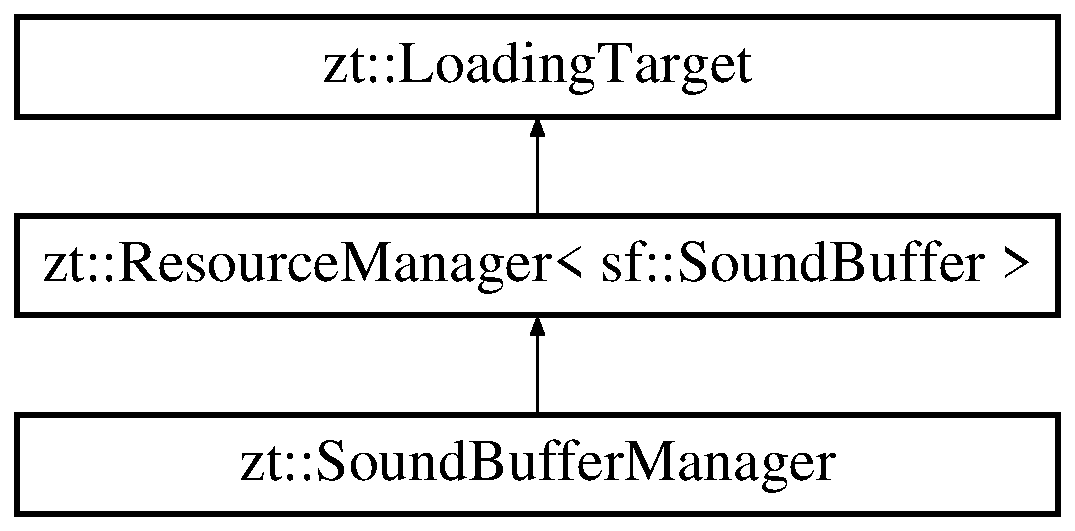
\includegraphics[height=3.000000cm]{classzt_1_1_sound_buffer_manager}
\end{center}
\end{figure}
\subsection*{Public Member Functions}
\begin{DoxyCompactItemize}
\item 
\mbox{\Hypertarget{classzt_1_1_sound_buffer_manager_a6e49792172f215b99908fdcb0ce43cf1}\label{classzt_1_1_sound_buffer_manager_a6e49792172f215b99908fdcb0ce43cf1}} 
virtual void {\bfseries load\+From\+File} (const std\+::string \&name, const std\+::string \&file)
\item 
\mbox{\Hypertarget{classzt_1_1_sound_buffer_manager_af9f12e257943e82ed68d1272a6e053af}\label{classzt_1_1_sound_buffer_manager_af9f12e257943e82ed68d1272a6e053af}} 
virtual void {\bfseries load\+From\+Memory} (const std\+::string \&name, const void $\ast$data, std\+::size\+\_\+t size)
\end{DoxyCompactItemize}
\subsection*{Additional Inherited Members}


\subsection{Detailed Description}
Resource manager for sf\+::\+Sound\+Buffer. 

The documentation for this class was generated from the following file\+:\begin{DoxyCompactItemize}
\item 
include/\+Zelta/\+Core/Sound\+Buffer\+Manager.\+hpp\end{DoxyCompactItemize}

\hypertarget{classzt_1_1_task}{}\section{zt\+:\+:Task Class Reference}
\label{classzt_1_1_task}\index{zt\+::\+Task@{zt\+::\+Task}}


A \hyperlink{classzt_1_1_task}{Task} is a unit of work.  




{\ttfamily \#include $<$Task.\+hpp$>$}

\subsection*{Public Member Functions}
\begin{DoxyCompactItemize}
\item 
virtual bool \hyperlink{classzt_1_1_task_a6026a3bc7552bd86653f1168919ae7ab}{work} ()=0
\end{DoxyCompactItemize}


\subsection{Detailed Description}
A \hyperlink{classzt_1_1_task}{Task} is a unit of work. 

If you need something to be executed in a different thread you can use \hyperlink{classzt_1_1_task}{Task} and \hyperlink{classzt_1_1_task_pool}{Task\+Pool} classes.

\begin{DoxySeeAlso}{See also}
\hyperlink{classzt_1_1_task_pool}{Task\+Pool} 
\end{DoxySeeAlso}


\subsection{Member Function Documentation}
\mbox{\Hypertarget{classzt_1_1_task_a6026a3bc7552bd86653f1168919ae7ab}\label{classzt_1_1_task_a6026a3bc7552bd86653f1168919ae7ab}} 
\index{zt\+::\+Task@{zt\+::\+Task}!work@{work}}
\index{work@{work}!zt\+::\+Task@{zt\+::\+Task}}
\subsubsection{\texorpdfstring{work()}{work()}}
{\footnotesize\ttfamily virtual bool zt\+::\+Task\+::work (\begin{DoxyParamCaption}{ }\end{DoxyParamCaption})\hspace{0.3cm}{\ttfamily [pure virtual]}}

\begin{DoxyReturn}{Returns}
True if the task is finished. 
\end{DoxyReturn}


The documentation for this class was generated from the following file\+:\begin{DoxyCompactItemize}
\item 
include/\+Zelta/\+Concurrency/Task.\+hpp\end{DoxyCompactItemize}

\hypertarget{classzt_1_1_task_pool}{}\section{zt\+:\+:Task\+Pool Class Reference}
\label{classzt_1_1_task_pool}\index{zt\+::\+Task\+Pool@{zt\+::\+Task\+Pool}}


A \hyperlink{classzt_1_1_task_pool}{Task\+Pool} keeps a set of workers (threads represented by the \hyperlink{classzt_1_1_worker}{Worker} class). You can enqueue tasks in the \hyperlink{classzt_1_1_task_pool}{Task\+Pool} and they will be executed when a worker is free.  




{\ttfamily \#include $<$Task\+Pool.\+hpp$>$}

\subsection*{Public Member Functions}
\begin{DoxyCompactItemize}
\item 
\hyperlink{classzt_1_1_task_pool_a20b14ff66aaf67a035dd7394e7266ee0}{Task\+Pool} (unsigned int threads=2)
\item 
void \hyperlink{classzt_1_1_task_pool_a966bbcbfbc550c1324772d90c1c70f1b}{add\+Task} (\hyperlink{classzt_1_1_task}{Task} \&task)
\item 
void \hyperlink{classzt_1_1_task_pool_a39276f6d847af21e7c6eff52a4712fea}{join} ()
\item 
\mbox{\Hypertarget{classzt_1_1_task_pool_ad9e5feffedd371d5ef1f0bfce8cef5c4}\label{classzt_1_1_task_pool_ad9e5feffedd371d5ef1f0bfce8cef5c4}} 
void {\bfseries stop} ()
\end{DoxyCompactItemize}
\subsection*{Protected Member Functions}
\begin{DoxyCompactItemize}
\item 
void \hyperlink{classzt_1_1_task_pool_a1b03b3bf318d4873e9109cd6c9ba43b4}{work} ()
\end{DoxyCompactItemize}


\subsection{Detailed Description}
A \hyperlink{classzt_1_1_task_pool}{Task\+Pool} keeps a set of workers (threads represented by the \hyperlink{classzt_1_1_worker}{Worker} class). You can enqueue tasks in the \hyperlink{classzt_1_1_task_pool}{Task\+Pool} and they will be executed when a worker is free. 

To create a task just inherit from \hyperlink{classzt_1_1_task}{Task} and implement in the \hyperlink{classzt_1_1_task_pool_a1b03b3bf318d4873e9109cd6c9ba43b4}{work()} method the code you want to execute in a different thread. The \hyperlink{classzt_1_1_task_pool_a1b03b3bf318d4873e9109cd6c9ba43b4}{work()} method must return true if it has finished the task so that the worker gets released. Then, instance the \hyperlink{classzt_1_1_task}{Task} and add it to a \hyperlink{classzt_1_1_task_pool}{Task\+Pool} with \hyperlink{classzt_1_1_task_pool_a966bbcbfbc550c1324772d90c1c70f1b}{add\+Task()}. The task will be executed as soon as a \hyperlink{classzt_1_1_worker}{Worker} is free. 

\subsection{Constructor \& Destructor Documentation}
\mbox{\Hypertarget{classzt_1_1_task_pool_a20b14ff66aaf67a035dd7394e7266ee0}\label{classzt_1_1_task_pool_a20b14ff66aaf67a035dd7394e7266ee0}} 
\index{zt\+::\+Task\+Pool@{zt\+::\+Task\+Pool}!Task\+Pool@{Task\+Pool}}
\index{Task\+Pool@{Task\+Pool}!zt\+::\+Task\+Pool@{zt\+::\+Task\+Pool}}
\subsubsection{\texorpdfstring{Task\+Pool()}{TaskPool()}}
{\footnotesize\ttfamily zt\+::\+Task\+Pool\+::\+Task\+Pool (\begin{DoxyParamCaption}\item[{unsigned int}]{threads = {\ttfamily 2} }\end{DoxyParamCaption})}

Creates a \hyperlink{classzt_1_1_task_pool}{Task\+Pool} with a certain amount of threads. 
\begin{DoxyParams}{Parameters}
{\em threads} & \\
\hline
\end{DoxyParams}


\subsection{Member Function Documentation}
\mbox{\Hypertarget{classzt_1_1_task_pool_a966bbcbfbc550c1324772d90c1c70f1b}\label{classzt_1_1_task_pool_a966bbcbfbc550c1324772d90c1c70f1b}} 
\index{zt\+::\+Task\+Pool@{zt\+::\+Task\+Pool}!add\+Task@{add\+Task}}
\index{add\+Task@{add\+Task}!zt\+::\+Task\+Pool@{zt\+::\+Task\+Pool}}
\subsubsection{\texorpdfstring{add\+Task()}{addTask()}}
{\footnotesize\ttfamily void zt\+::\+Task\+Pool\+::add\+Task (\begin{DoxyParamCaption}\item[{\hyperlink{classzt_1_1_task}{Task} \&}]{task }\end{DoxyParamCaption})}

Adds a new task to the queue. 
\begin{DoxyParams}{Parameters}
{\em task} & \\
\hline
\end{DoxyParams}
\mbox{\Hypertarget{classzt_1_1_task_pool_a39276f6d847af21e7c6eff52a4712fea}\label{classzt_1_1_task_pool_a39276f6d847af21e7c6eff52a4712fea}} 
\index{zt\+::\+Task\+Pool@{zt\+::\+Task\+Pool}!join@{join}}
\index{join@{join}!zt\+::\+Task\+Pool@{zt\+::\+Task\+Pool}}
\subsubsection{\texorpdfstring{join()}{join()}}
{\footnotesize\ttfamily void zt\+::\+Task\+Pool\+::join (\begin{DoxyParamCaption}{ }\end{DoxyParamCaption})}

Waits until the manager thread and the \hyperlink{classzt_1_1_worker}{Worker} threads are done. \mbox{\Hypertarget{classzt_1_1_task_pool_a1b03b3bf318d4873e9109cd6c9ba43b4}\label{classzt_1_1_task_pool_a1b03b3bf318d4873e9109cd6c9ba43b4}} 
\index{zt\+::\+Task\+Pool@{zt\+::\+Task\+Pool}!work@{work}}
\index{work@{work}!zt\+::\+Task\+Pool@{zt\+::\+Task\+Pool}}
\subsubsection{\texorpdfstring{work()}{work()}}
{\footnotesize\ttfamily void zt\+::\+Task\+Pool\+::work (\begin{DoxyParamCaption}{ }\end{DoxyParamCaption})\hspace{0.3cm}{\ttfamily [protected]}}

Manages the queue. This method is executed in a different thread and keeps running until you call stop(). Workers notificates this thread when they are free so that it can send them new tasks. 

The documentation for this class was generated from the following file\+:\begin{DoxyCompactItemize}
\item 
include/\+Zelta/\+Concurrency/Task\+Pool.\+hpp\end{DoxyCompactItemize}

\hypertarget{classzt_1_1_text}{}\section{zt\+:\+:Text Class Reference}
\label{classzt_1_1_text}\index{zt\+::\+Text@{zt\+::\+Text}}
Inheritance diagram for zt\+:\+:Text\+:\begin{figure}[H]
\begin{center}
\leavevmode
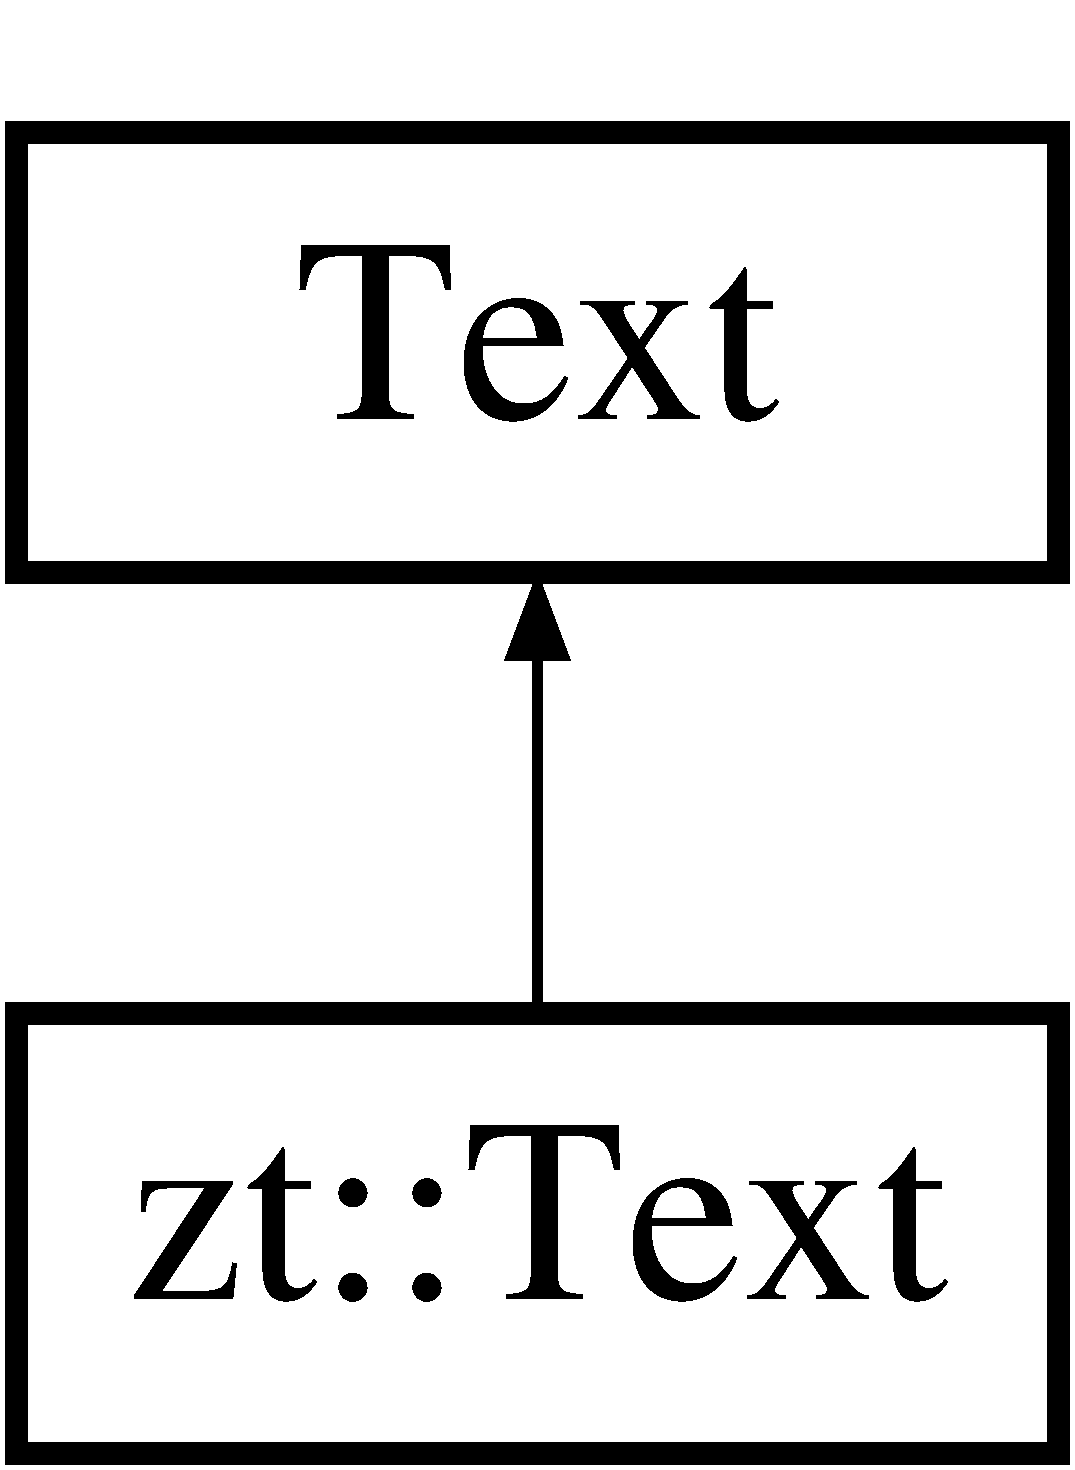
\includegraphics[height=2.000000cm]{classzt_1_1_text}
\end{center}
\end{figure}
\subsection*{Public Member Functions}
\begin{DoxyCompactItemize}
\item 
\mbox{\Hypertarget{classzt_1_1_text_a3911db18eb027d801bac56dff1ea3bb5}\label{classzt_1_1_text_a3911db18eb027d801bac56dff1ea3bb5}} 
virtual void {\bfseries translated} ()
\end{DoxyCompactItemize}


The documentation for this class was generated from the following file\+:\begin{DoxyCompactItemize}
\item 
include/\+Zelta/\+Internationalization/Text.\+hpp\end{DoxyCompactItemize}

\hypertarget{classzt_1_1_texture_manager}{}\section{zt\+:\+:Texture\+Manager Class Reference}
\label{classzt_1_1_texture_manager}\index{zt\+::\+Texture\+Manager@{zt\+::\+Texture\+Manager}}


Resource manager for sf\+::\+Texture.  




{\ttfamily \#include $<$Texture\+Manager.\+hpp$>$}

Inheritance diagram for zt\+:\+:Texture\+Manager\+:\begin{figure}[H]
\begin{center}
\leavevmode
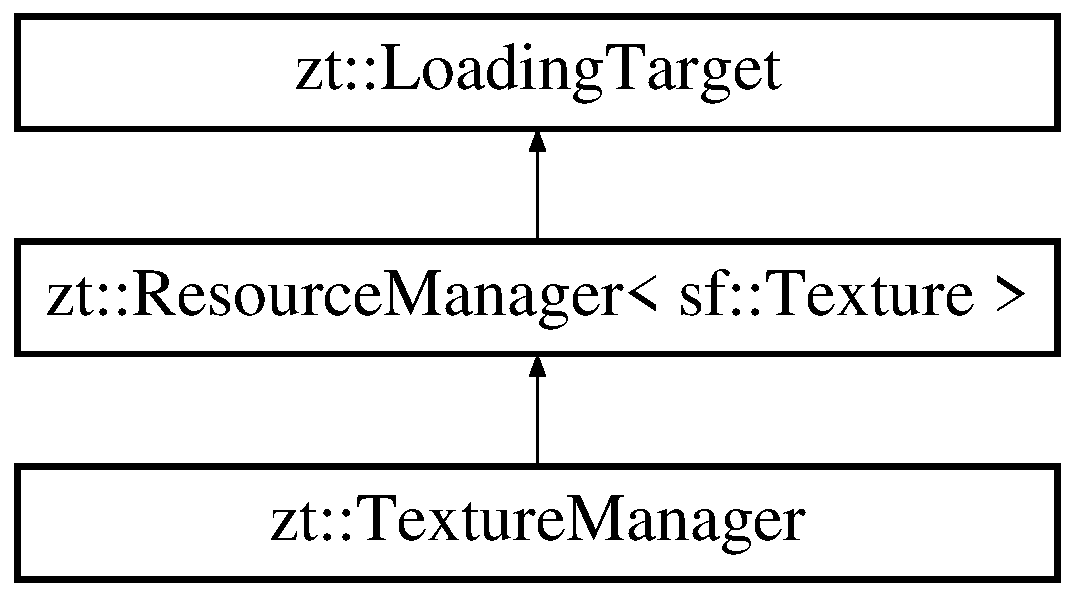
\includegraphics[height=3.000000cm]{classzt_1_1_texture_manager}
\end{center}
\end{figure}
\subsection*{Public Member Functions}
\begin{DoxyCompactItemize}
\item 
\mbox{\Hypertarget{classzt_1_1_texture_manager_a879750a20bccb880621017f94f94ced6}\label{classzt_1_1_texture_manager_a879750a20bccb880621017f94f94ced6}} 
virtual void {\bfseries load\+From\+File} (const std\+::string \&name, const std\+::string \&file)
\item 
\mbox{\Hypertarget{classzt_1_1_texture_manager_a872e10acf220cd9a77b498b9f30978d6}\label{classzt_1_1_texture_manager_a872e10acf220cd9a77b498b9f30978d6}} 
virtual void {\bfseries load\+From\+Memory} (const std\+::string \&name, const void $\ast$data, std\+::size\+\_\+t size)
\end{DoxyCompactItemize}
\subsection*{Additional Inherited Members}


\subsection{Detailed Description}
Resource manager for sf\+::\+Texture. 

The documentation for this class was generated from the following file\+:\begin{DoxyCompactItemize}
\item 
include/\+Zelta/\+Core/Texture\+Manager.\+hpp\end{DoxyCompactItemize}

\hypertarget{classzt_1_1tiled_1_1_tile}{}\section{zt\+:\+:tiled\+:\+:Tile Class Reference}
\label{classzt_1_1tiled_1_1_tile}\index{zt\+::tiled\+::\+Tile@{zt\+::tiled\+::\+Tile}}
\subsection*{Public Member Functions}
\begin{DoxyCompactItemize}
\item 
\mbox{\Hypertarget{classzt_1_1tiled_1_1_tile_aa178268dae96e986737e3f1753da0aaa}\label{classzt_1_1tiled_1_1_tile_aa178268dae96e986737e3f1753da0aaa}} 
{\bfseries Tile} (int gid)
\item 
\mbox{\Hypertarget{classzt_1_1tiled_1_1_tile_a2b9b5baee7c8816366bc553a84b24c77}\label{classzt_1_1tiled_1_1_tile_a2b9b5baee7c8816366bc553a84b24c77}} 
int {\bfseries get\+G\+ID} () const
\end{DoxyCompactItemize}


The documentation for this class was generated from the following file\+:\begin{DoxyCompactItemize}
\item 
include/\+Zelta/\+Tile\+Engine/\+Tiled\+Loader/Tile.\+hpp\end{DoxyCompactItemize}

\hypertarget{classzt_1_1_tile_container}{}\section{zt\+:\+:Tile\+Container$<$ T $>$ Class Template Reference}
\label{classzt_1_1_tile_container}\index{zt\+::\+Tile\+Container$<$ T $>$@{zt\+::\+Tile\+Container$<$ T $>$}}
\subsection*{Public Attributes}
\begin{DoxyCompactItemize}
\item 
\mbox{\Hypertarget{classzt_1_1_tile_container_aab3b478c2ba149552d49fb7dc75f10af}\label{classzt_1_1_tile_container_aab3b478c2ba149552d49fb7dc75f10af}} 
T {\bfseries tile}
\item 
\mbox{\Hypertarget{classzt_1_1_tile_container_a0c08596908cd40992020b9d61411cfb9}\label{classzt_1_1_tile_container_a0c08596908cd40992020b9d61411cfb9}} 
bool {\bfseries empty}
\end{DoxyCompactItemize}


The documentation for this class was generated from the following file\+:\begin{DoxyCompactItemize}
\item 
include/\+Zelta/\+Tile\+Engine/Tilemap\+Layer.\+hpp\end{DoxyCompactItemize}

\hypertarget{classzt_1_1tiled_1_1_tiled_loader}{}\section{zt\+:\+:tiled\+:\+:Tiled\+Loader Class Reference}
\label{classzt_1_1tiled_1_1_tiled_loader}\index{zt\+::tiled\+::\+Tiled\+Loader@{zt\+::tiled\+::\+Tiled\+Loader}}
\subsection*{Public Member Functions}
\begin{DoxyCompactItemize}
\item 
\mbox{\Hypertarget{classzt_1_1tiled_1_1_tiled_loader_a4dcb166aef23c58af56d06ecb658240f}\label{classzt_1_1tiled_1_1_tiled_loader_a4dcb166aef23c58af56d06ecb658240f}} 
\hyperlink{classzt_1_1tiled_1_1_map}{Map} {\bfseries load\+From\+File} (const std\+::string \&file)
\item 
\mbox{\Hypertarget{classzt_1_1tiled_1_1_tiled_loader_a1f893b1c6e8eb87c494468bad25fd08d}\label{classzt_1_1tiled_1_1_tiled_loader_a1f893b1c6e8eb87c494468bad25fd08d}} 
virtual void {\bfseries size\+Loaded} (sf\+::\+Vector2u map\+Size, const sf\+::\+Vector2u \&tile\+Size)
\item 
\mbox{\Hypertarget{classzt_1_1tiled_1_1_tiled_loader_abe1f0dfb3a7028bbc6d7e5ca0eefe1d1}\label{classzt_1_1tiled_1_1_tiled_loader_abe1f0dfb3a7028bbc6d7e5ca0eefe1d1}} 
virtual void {\bfseries layer\+Loaded} (\hyperlink{classzt_1_1tiled_1_1_layer}{Layer} layer)
\item 
\mbox{\Hypertarget{classzt_1_1tiled_1_1_tiled_loader_a9dc3e335436c2a099c109617ea9ef366}\label{classzt_1_1tiled_1_1_tiled_loader_a9dc3e335436c2a099c109617ea9ef366}} 
virtual void {\bfseries object\+Layer\+Loaded} (\hyperlink{classzt_1_1tiled_1_1_object_layer}{Object\+Layer} object\+Group)
\end{DoxyCompactItemize}


The documentation for this class was generated from the following file\+:\begin{DoxyCompactItemize}
\item 
include/\+Zelta/\+Tile\+Engine/\+Tiled\+Loader/Tiled\+Loader.\+hpp\end{DoxyCompactItemize}

\hypertarget{classzt_1_1_tilemap_layer}{}\section{zt\+:\+:Tilemap\+Layer$<$ T $>$ Class Template Reference}
\label{classzt_1_1_tilemap_layer}\index{zt\+::\+Tilemap\+Layer$<$ T $>$@{zt\+::\+Tilemap\+Layer$<$ T $>$}}
Inheritance diagram for zt\+:\+:Tilemap\+Layer$<$ T $>$\+:\begin{figure}[H]
\begin{center}
\leavevmode
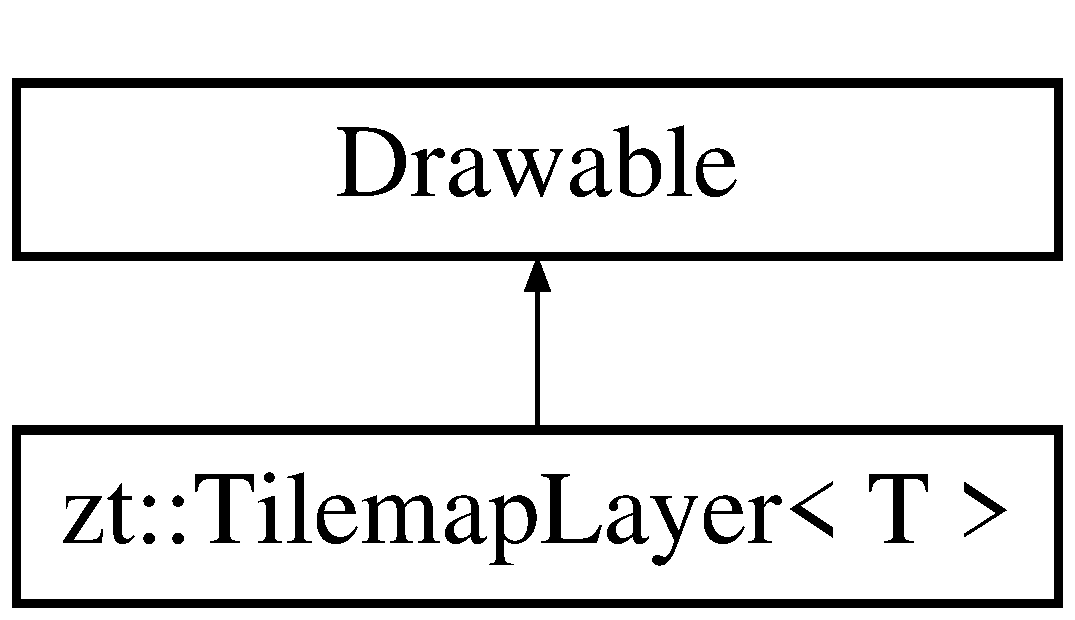
\includegraphics[height=2.000000cm]{classzt_1_1_tilemap_layer}
\end{center}
\end{figure}
\subsection*{Public Member Functions}
\begin{DoxyCompactItemize}
\item 
\mbox{\Hypertarget{classzt_1_1_tilemap_layer_afe899acb9ffba9fba70e0913595f124c}\label{classzt_1_1_tilemap_layer_afe899acb9ffba9fba70e0913595f124c}} 
void {\bfseries set\+Size} (const sf\+::\+Vector2u \&size)
\item 
\mbox{\Hypertarget{classzt_1_1_tilemap_layer_a8990bba160dd50c39a6abcf803bb58e0}\label{classzt_1_1_tilemap_layer_a8990bba160dd50c39a6abcf803bb58e0}} 
const sf\+::\+Vector2u \& {\bfseries get\+Size} () const
\item 
\mbox{\Hypertarget{classzt_1_1_tilemap_layer_a51c80b285c7128b1ff48f5efe34b302f}\label{classzt_1_1_tilemap_layer_a51c80b285c7128b1ff48f5efe34b302f}} 
void {\bfseries set\+Tile\+Size} (const sf\+::\+Vector2u \&tile\+Size)
\item 
\mbox{\Hypertarget{classzt_1_1_tilemap_layer_a0711254a5302e3cce7d19f269a48bff7}\label{classzt_1_1_tilemap_layer_a0711254a5302e3cce7d19f269a48bff7}} 
const sf\+::\+Vector2u \& {\bfseries get\+Tile\+Size} () const
\item 
\mbox{\Hypertarget{classzt_1_1_tilemap_layer_a18d1e2f04247e83bac25d5ec03870b8b}\label{classzt_1_1_tilemap_layer_a18d1e2f04247e83bac25d5ec03870b8b}} 
void {\bfseries update\+View} (const sf\+::\+View \&view)
\item 
\mbox{\Hypertarget{classzt_1_1_tilemap_layer_a187ec1100dcd2f02eac6f2ba32d1bf4e}\label{classzt_1_1_tilemap_layer_a187ec1100dcd2f02eac6f2ba32d1bf4e}} 
void {\bfseries draw} (sf\+::\+Render\+Target \&target, sf\+::\+Render\+States states) const
\item 
\mbox{\Hypertarget{classzt_1_1_tilemap_layer_a042b846c7958ac5fe1f82250c6cc1d3f}\label{classzt_1_1_tilemap_layer_a042b846c7958ac5fe1f82250c6cc1d3f}} 
std\+::pair$<$ int, T $\ast$ $>$ {\bfseries add\+Tile} (const T \&tile, const sf\+::\+Vector2u \&tile\+Position)
\item 
std\+::pair$<$ int, T $\ast$ $>$ \hyperlink{classzt_1_1_tilemap_layer_a6fe52aa49bd4965ac7df8a6db0187f5a}{add\+Tile} (const sf\+::\+Vector2u \&tile\+Position)
\begin{DoxyCompactList}\small\item\em Add a tile in a given position. \end{DoxyCompactList}\item 
\mbox{\Hypertarget{classzt_1_1_tilemap_layer_aaa84d473ece41766d7eab924821b3ed8}\label{classzt_1_1_tilemap_layer_aaa84d473ece41766d7eab924821b3ed8}} 
unsigned int {\bfseries count\+Tiles} () const
\item 
\mbox{\Hypertarget{classzt_1_1_tilemap_layer_af8beb5aa8873b00235677aa86d01271e}\label{classzt_1_1_tilemap_layer_af8beb5aa8873b00235677aa86d01271e}} 
void {\bfseries set\+Name} (const std\+::wstring \&name)
\item 
\mbox{\Hypertarget{classzt_1_1_tilemap_layer_a1d892a157ae743bbcd65632dbc10b973}\label{classzt_1_1_tilemap_layer_a1d892a157ae743bbcd65632dbc10b973}} 
const std\+::wstring \& {\bfseries get\+Name} () const
\item 
\mbox{\Hypertarget{classzt_1_1_tilemap_layer_a90f1e2ffac9764bf50813a252d4ef859}\label{classzt_1_1_tilemap_layer_a90f1e2ffac9764bf50813a252d4ef859}} 
bool {\bfseries is\+Empty} (int x, int y)
\item 
\mbox{\Hypertarget{classzt_1_1_tilemap_layer_a7d780310f2514eceb3bfdec5c50913fc}\label{classzt_1_1_tilemap_layer_a7d780310f2514eceb3bfdec5c50913fc}} 
T \& {\bfseries get\+Tile} (int x, int y)
\end{DoxyCompactItemize}


\subsection{Member Function Documentation}
\mbox{\Hypertarget{classzt_1_1_tilemap_layer_a6fe52aa49bd4965ac7df8a6db0187f5a}\label{classzt_1_1_tilemap_layer_a6fe52aa49bd4965ac7df8a6db0187f5a}} 
\index{zt\+::\+Tilemap\+Layer@{zt\+::\+Tilemap\+Layer}!add\+Tile@{add\+Tile}}
\index{add\+Tile@{add\+Tile}!zt\+::\+Tilemap\+Layer@{zt\+::\+Tilemap\+Layer}}
\subsubsection{\texorpdfstring{add\+Tile()}{addTile()}}
{\footnotesize\ttfamily template$<$class T$>$ \\
std\+::pair$<$int, T$\ast$$>$ \hyperlink{classzt_1_1_tilemap_layer}{zt\+::\+Tilemap\+Layer}$<$ T $>$\+::add\+Tile (\begin{DoxyParamCaption}\item[{const sf\+::\+Vector2u \&}]{tile\+Position }\end{DoxyParamCaption})\hspace{0.3cm}{\ttfamily [inline]}}



Add a tile in a given position. 


\begin{DoxyParams}{Parameters}
{\em tile\+Position} & Position (measured in tiles). \\
\hline
\end{DoxyParams}
\begin{DoxyReturn}{Returns}
Returns a pair. The first element is the position of the tile in the vector. The second element is a pointer to the new tile. 
\end{DoxyReturn}


The documentation for this class was generated from the following file\+:\begin{DoxyCompactItemize}
\item 
include/\+Zelta/\+Tile\+Engine/Tilemap\+Layer.\+hpp\end{DoxyCompactItemize}

\hypertarget{classzt_1_1_tilemap_renderer}{}\section{zt\+:\+:Tilemap\+Renderer$<$ T $>$ Class Template Reference}
\label{classzt_1_1_tilemap_renderer}\index{zt\+::\+Tilemap\+Renderer$<$ T $>$@{zt\+::\+Tilemap\+Renderer$<$ T $>$}}
Inheritance diagram for zt\+:\+:Tilemap\+Renderer$<$ T $>$\+:\begin{figure}[H]
\begin{center}
\leavevmode
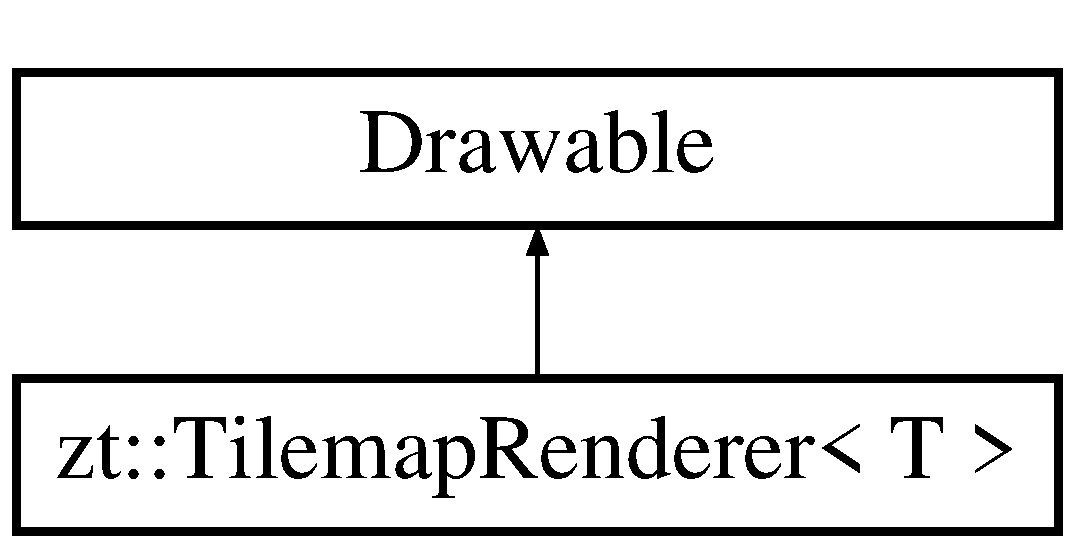
\includegraphics[height=2.000000cm]{classzt_1_1_tilemap_renderer}
\end{center}
\end{figure}
\subsection*{Public Member Functions}
\begin{DoxyCompactItemize}
\item 
\mbox{\Hypertarget{classzt_1_1_tilemap_renderer_a9feb81534e16c96ce3e3ee5670662daa}\label{classzt_1_1_tilemap_renderer_a9feb81534e16c96ce3e3ee5670662daa}} 
void {\bfseries set\+Size} (const sf\+::\+Vector2u \&\hyperlink{classzt_1_1_tilemap_renderer_a41d82c316bae652d144415dcbb7b3fd0}{size})
\item 
\mbox{\Hypertarget{classzt_1_1_tilemap_renderer_a5cf40934d8a8bf79347a111b8f47268c}\label{classzt_1_1_tilemap_renderer_a5cf40934d8a8bf79347a111b8f47268c}} 
const sf\+::\+Vector2u \& {\bfseries get\+Size} () const
\item 
\mbox{\Hypertarget{classzt_1_1_tilemap_renderer_ad6f065fa9f0779c83017428e084f20ff}\label{classzt_1_1_tilemap_renderer_ad6f065fa9f0779c83017428e084f20ff}} 
virtual void {\bfseries draw} (sf\+::\+Render\+Target \&target, sf\+::\+Render\+States states) const
\item 
\mbox{\Hypertarget{classzt_1_1_tilemap_renderer_a62ff3f11368b2ee9de0d3b3c55e5b671}\label{classzt_1_1_tilemap_renderer_a62ff3f11368b2ee9de0d3b3c55e5b671}} 
virtual void {\bfseries add\+Layer} (\hyperlink{classzt_1_1_tilemap_layer}{Tilemap\+Layer}$<$ T $>$ layer)
\item 
\mbox{\Hypertarget{classzt_1_1_tilemap_renderer_a13eab06fa00e6017bc3754309d689ccb}\label{classzt_1_1_tilemap_renderer_a13eab06fa00e6017bc3754309d689ccb}} 
void {\bfseries update\+View} (const sf\+::\+View \&view)
\item 
\hyperlink{classzt_1_1_tilemap_layer}{Tilemap\+Layer}$<$ T $>$ \& \hyperlink{classzt_1_1_tilemap_renderer_ad6e938ecae5da3fc70c2e4e36254bf73}{get\+Layer\+By\+Name} (std\+::wstring name)
\end{DoxyCompactItemize}
\subsection*{Protected Attributes}
\begin{DoxyCompactItemize}
\item 
\mbox{\Hypertarget{classzt_1_1_tilemap_renderer_a41d82c316bae652d144415dcbb7b3fd0}\label{classzt_1_1_tilemap_renderer_a41d82c316bae652d144415dcbb7b3fd0}} 
sf\+::\+Vector2u \hyperlink{classzt_1_1_tilemap_renderer_a41d82c316bae652d144415dcbb7b3fd0}{size}
\begin{DoxyCompactList}\small\item\em Ancho y alto en tiles del mapa. \end{DoxyCompactList}\item 
\mbox{\Hypertarget{classzt_1_1_tilemap_renderer_aa6a529a25e69408699b76bcc25c892fb}\label{classzt_1_1_tilemap_renderer_aa6a529a25e69408699b76bcc25c892fb}} 
std\+::vector$<$ \hyperlink{classzt_1_1_tilemap_layer}{Tilemap\+Layer}$<$ T $>$ $>$ {\bfseries layers}
\item 
\mbox{\Hypertarget{classzt_1_1_tilemap_renderer_aef57126336a35de96de481267817224d}\label{classzt_1_1_tilemap_renderer_aef57126336a35de96de481267817224d}} 
sf\+::\+View {\bfseries view}
\end{DoxyCompactItemize}


\subsection{Member Function Documentation}
\mbox{\Hypertarget{classzt_1_1_tilemap_renderer_ad6e938ecae5da3fc70c2e4e36254bf73}\label{classzt_1_1_tilemap_renderer_ad6e938ecae5da3fc70c2e4e36254bf73}} 
\index{zt\+::\+Tilemap\+Renderer@{zt\+::\+Tilemap\+Renderer}!get\+Layer\+By\+Name@{get\+Layer\+By\+Name}}
\index{get\+Layer\+By\+Name@{get\+Layer\+By\+Name}!zt\+::\+Tilemap\+Renderer@{zt\+::\+Tilemap\+Renderer}}
\subsubsection{\texorpdfstring{get\+Layer\+By\+Name()}{getLayerByName()}}
{\footnotesize\ttfamily template$<$class T $>$ \\
\hyperlink{classzt_1_1_tilemap_layer}{Tilemap\+Layer}$<$T$>$\& \hyperlink{classzt_1_1_tilemap_renderer}{zt\+::\+Tilemap\+Renderer}$<$ T $>$\+::get\+Layer\+By\+Name (\begin{DoxyParamCaption}\item[{std\+::wstring}]{name }\end{DoxyParamCaption})\hspace{0.3cm}{\ttfamily [inline]}}

Devuelve una capa a partir de su nombre. Si no existe lanza una excepción. 
\begin{DoxyParams}{Parameters}
{\em name} & \\
\hline
\end{DoxyParams}
\begin{DoxyReturn}{Returns}
Capa. 
\end{DoxyReturn}


The documentation for this class was generated from the following file\+:\begin{DoxyCompactItemize}
\item 
include/\+Zelta/\+Tile\+Engine/Tilemap\+Renderer.\+hpp\end{DoxyCompactItemize}

\hypertarget{classzt_1_1_tileset}{}\section{zt\+:\+:Tileset Class Reference}
\label{classzt_1_1_tileset}\index{zt\+::\+Tileset@{zt\+::\+Tileset}}
\subsection*{Public Member Functions}
\begin{DoxyCompactItemize}
\item 
\mbox{\Hypertarget{classzt_1_1_tileset_aedae616d1a77443e22f6e1613946ec1b}\label{classzt_1_1_tileset_aedae616d1a77443e22f6e1613946ec1b}} 
const sf\+::\+Texture \& {\bfseries get\+Texture\+For\+Tile} (unsigned int i) const
\item 
\mbox{\Hypertarget{classzt_1_1_tileset_a6400f74fa3c1d51235715b07c743ed90}\label{classzt_1_1_tileset_a6400f74fa3c1d51235715b07c743ed90}} 
void {\bfseries create} (sf\+::\+Texture \&texture, const sf\+::\+Vector2u \&size)
\item 
\mbox{\Hypertarget{classzt_1_1_tileset_a19192046cbbe4f09d05058ca442a5360}\label{classzt_1_1_tileset_a19192046cbbe4f09d05058ca442a5360}} 
void {\bfseries create} (sf\+::\+Texture \&texture, const sf\+::\+Vector2u \&tiles, sf\+::\+Vector2f padding, sf\+::\+Vector2f margin)
\end{DoxyCompactItemize}


The documentation for this class was generated from the following file\+:\begin{DoxyCompactItemize}
\item 
include/\+Zelta/\+Tile\+Engine/Tileset.\+hpp\end{DoxyCompactItemize}

\hypertarget{classzt_1_1_vector2f}{}\section{zt\+:\+:Vector2f Class Reference}
\label{classzt_1_1_vector2f}\index{zt\+::\+Vector2f@{zt\+::\+Vector2f}}


Utility class for 2-\/dimensional vectors.  




{\ttfamily \#include $<$Vector2f.\+hpp$>$}

\subsection*{Public Member Functions}
\begin{DoxyCompactItemize}
\item 
\mbox{\Hypertarget{classzt_1_1_vector2f_a94fc942a263a91f4f33d2821ee9c8acd}\label{classzt_1_1_vector2f_a94fc942a263a91f4f33d2821ee9c8acd}} 
{\bfseries Vector2f} (float x, float y)
\item 
\mbox{\Hypertarget{classzt_1_1_vector2f_a50ad9da433750914c687db6ede87e0a7}\label{classzt_1_1_vector2f_a50ad9da433750914c687db6ede87e0a7}} 
{\bfseries Vector2f} (const sf\+::\+Vector2f \&v)
\item 
\mbox{\Hypertarget{classzt_1_1_vector2f_a94ee9212d0ccaf6e88fd22f400925d24}\label{classzt_1_1_vector2f_a94ee9212d0ccaf6e88fd22f400925d24}} 
float {\bfseries getX} () const
\item 
\mbox{\Hypertarget{classzt_1_1_vector2f_a4c33e6e5f654d4e330ec802a3eefcd96}\label{classzt_1_1_vector2f_a4c33e6e5f654d4e330ec802a3eefcd96}} 
float {\bfseries getY} () const
\item 
\mbox{\Hypertarget{classzt_1_1_vector2f_abe058bbefd3d3490ed56e0b220724472}\label{classzt_1_1_vector2f_abe058bbefd3d3490ed56e0b220724472}} 
float {\bfseries length} () const
\item 
\mbox{\Hypertarget{classzt_1_1_vector2f_adf28079a299c65def555c97d3fb9c51d}\label{classzt_1_1_vector2f_adf28079a299c65def555c97d3fb9c51d}} 
void {\bfseries setX} (float x)
\item 
\mbox{\Hypertarget{classzt_1_1_vector2f_a6e6f512e24654940ca3cc20c97a24871}\label{classzt_1_1_vector2f_a6e6f512e24654940ca3cc20c97a24871}} 
void {\bfseries setY} (float y)
\item 
\mbox{\Hypertarget{classzt_1_1_vector2f_aa3318b77bb7ace0065c93f1d110b189f}\label{classzt_1_1_vector2f_aa3318b77bb7ace0065c93f1d110b189f}} 
void {\bfseries set} (float x, float y)
\item 
void \hyperlink{classzt_1_1_vector2f_a2992fead31cd872fbb7d2bda8271cdad}{normalize} ()
\begin{DoxyCompactList}\small\item\em Normalizes the vector. \end{DoxyCompactList}\item 
\hyperlink{classzt_1_1_vector2f}{Vector2f} \& \hyperlink{classzt_1_1_vector2f_ac87f5252d360bf9bad0934acbaa4cc07}{add} (const \hyperlink{classzt_1_1_vector2f}{Vector2f} \&other)
\begin{DoxyCompactList}\small\item\em Adds the other vector to this one. \end{DoxyCompactList}\item 
\hyperlink{classzt_1_1_vector2f}{Vector2f} \& \hyperlink{classzt_1_1_vector2f_aada2302369ae96e18db8362768702bd0}{multiply} (float num)
\begin{DoxyCompactList}\small\item\em Multiply the vector by a scalar. \end{DoxyCompactList}\item 
\hyperlink{classzt_1_1_vector2f}{Vector2f} \& \hyperlink{classzt_1_1_vector2f_a72873ae6ba73ade6dcabe23f482b4f82}{multiply} (float x, float y)
\begin{DoxyCompactList}\small\item\em Multiply the vector by two scalars. \end{DoxyCompactList}\item 
\hyperlink{classzt_1_1_vector2f}{Vector2f} \& \hyperlink{classzt_1_1_vector2f_a97aab9087dc306b6a8b9c61fa84e98de}{rotate} (float angle)
\begin{DoxyCompactList}\small\item\em Rotates de vector. \end{DoxyCompactList}\item 
\hyperlink{classzt_1_1_vector2f}{Vector2f} \hyperlink{classzt_1_1_vector2f_a46f3e0b08f9ea3c9ec0f1c0670f82ebc}{normalized} () const
\begin{DoxyCompactList}\small\item\em Returns the normalized vector. \end{DoxyCompactList}\item 
\hyperlink{classzt_1_1_vector3f}{Vector3f} \hyperlink{classzt_1_1_vector2f_a51b847203bcda779189114905d1dc77d}{cross} (const \hyperlink{classzt_1_1_vector2f}{Vector2f} \&other) const
\begin{DoxyCompactList}\small\item\em Returns the cross product. \end{DoxyCompactList}\item 
float \hyperlink{classzt_1_1_vector2f_a8141042fa92a5138e5d435505882d122}{dot} (const \hyperlink{classzt_1_1_vector2f}{Vector2f} \&other) const
\begin{DoxyCompactList}\small\item\em Returns the dot product. \end{DoxyCompactList}\item 
\hyperlink{classzt_1_1_vector2f}{Vector2f} \hyperlink{classzt_1_1_vector2f_a9455159e20935fee1c3fd46d5c138caa}{plus} (const \hyperlink{classzt_1_1_vector2f}{Vector2f} \&other) const
\begin{DoxyCompactList}\small\item\em Adds this vector to other and returns the result. \end{DoxyCompactList}\item 
\hyperlink{classzt_1_1_vector2f}{Vector2f} \hyperlink{classzt_1_1_vector2f_a69478760accc84d5de3867c899499f3a}{minus} (const \hyperlink{classzt_1_1_vector2f}{Vector2f} \&other) const
\begin{DoxyCompactList}\small\item\em Substracts other vector to thisand returns the result. \end{DoxyCompactList}\item 
\hyperlink{classzt_1_1_vector2f}{Vector2f} \hyperlink{classzt_1_1_vector2f_a158fe50fd17f2a0ee72a6add6a33ae93}{multiplied} (float s) const
\begin{DoxyCompactList}\small\item\em Multiply the vector by a scalar. \end{DoxyCompactList}\item 
\hyperlink{classzt_1_1_vector2f}{Vector2f} \hyperlink{classzt_1_1_vector2f_aadee7c951439eb7953256e5f5704e28a}{multiplied} (float x, float y) const
\begin{DoxyCompactList}\small\item\em Multiply the vector by two scalars. \end{DoxyCompactList}\item 
\hyperlink{classzt_1_1_vector2f}{Vector2f} \hyperlink{classzt_1_1_vector2f_a1b301634478a665f0e0e7cacdc568cac}{rotated} (float angle) const
\begin{DoxyCompactList}\small\item\em Returns a new rotated vector. \end{DoxyCompactList}\item 
float \hyperlink{classzt_1_1_vector2f_a4449e55fef14e503d832831b97d2f949}{get\+Angle} () const
\item 
\hyperlink{classzt_1_1_vector2f}{Vector2f} \hyperlink{classzt_1_1_vector2f_a2aa1ef32f78d6399891f6318e9a0cd3c}{to} (const \hyperlink{classzt_1_1_vector2f}{Vector2f} \&other) const
\item 
sf\+::\+Vector2f \hyperlink{classzt_1_1_vector2f_aebb473f59fd05176a89031cad7b5e13a}{to\+Sfml} () const
\end{DoxyCompactItemize}


\subsection{Detailed Description}
Utility class for 2-\/dimensional vectors. 

\subsection{Member Function Documentation}
\mbox{\Hypertarget{classzt_1_1_vector2f_ac87f5252d360bf9bad0934acbaa4cc07}\label{classzt_1_1_vector2f_ac87f5252d360bf9bad0934acbaa4cc07}} 
\index{zt\+::\+Vector2f@{zt\+::\+Vector2f}!add@{add}}
\index{add@{add}!zt\+::\+Vector2f@{zt\+::\+Vector2f}}
\subsubsection{\texorpdfstring{add()}{add()}}
{\footnotesize\ttfamily \hyperlink{classzt_1_1_vector2f}{Vector2f}\& zt\+::\+Vector2f\+::add (\begin{DoxyParamCaption}\item[{const \hyperlink{classzt_1_1_vector2f}{Vector2f} \&}]{other }\end{DoxyParamCaption})}



Adds the other vector to this one. 


\begin{DoxyParams}{Parameters}
{\em other} & \\
\hline
\end{DoxyParams}
\begin{DoxyReturn}{Returns}
Returns this vector. 
\end{DoxyReturn}
\mbox{\Hypertarget{classzt_1_1_vector2f_a51b847203bcda779189114905d1dc77d}\label{classzt_1_1_vector2f_a51b847203bcda779189114905d1dc77d}} 
\index{zt\+::\+Vector2f@{zt\+::\+Vector2f}!cross@{cross}}
\index{cross@{cross}!zt\+::\+Vector2f@{zt\+::\+Vector2f}}
\subsubsection{\texorpdfstring{cross()}{cross()}}
{\footnotesize\ttfamily \hyperlink{classzt_1_1_vector3f}{Vector3f} zt\+::\+Vector2f\+::cross (\begin{DoxyParamCaption}\item[{const \hyperlink{classzt_1_1_vector2f}{Vector2f} \&}]{other }\end{DoxyParamCaption}) const}



Returns the cross product. 


\begin{DoxyParams}{Parameters}
{\em other} & Other vector. \\
\hline
\end{DoxyParams}
\begin{DoxyReturn}{Returns}
Cross product (3d vector). 
\end{DoxyReturn}
\mbox{\Hypertarget{classzt_1_1_vector2f_a8141042fa92a5138e5d435505882d122}\label{classzt_1_1_vector2f_a8141042fa92a5138e5d435505882d122}} 
\index{zt\+::\+Vector2f@{zt\+::\+Vector2f}!dot@{dot}}
\index{dot@{dot}!zt\+::\+Vector2f@{zt\+::\+Vector2f}}
\subsubsection{\texorpdfstring{dot()}{dot()}}
{\footnotesize\ttfamily float zt\+::\+Vector2f\+::dot (\begin{DoxyParamCaption}\item[{const \hyperlink{classzt_1_1_vector2f}{Vector2f} \&}]{other }\end{DoxyParamCaption}) const}



Returns the dot product. 


\begin{DoxyParams}{Parameters}
{\em other} & Other vector. \\
\hline
\end{DoxyParams}
\begin{DoxyReturn}{Returns}
Dot product. 
\end{DoxyReturn}
\mbox{\Hypertarget{classzt_1_1_vector2f_a4449e55fef14e503d832831b97d2f949}\label{classzt_1_1_vector2f_a4449e55fef14e503d832831b97d2f949}} 
\index{zt\+::\+Vector2f@{zt\+::\+Vector2f}!get\+Angle@{get\+Angle}}
\index{get\+Angle@{get\+Angle}!zt\+::\+Vector2f@{zt\+::\+Vector2f}}
\subsubsection{\texorpdfstring{get\+Angle()}{getAngle()}}
{\footnotesize\ttfamily float zt\+::\+Vector2f\+::get\+Angle (\begin{DoxyParamCaption}{ }\end{DoxyParamCaption}) const}

\begin{DoxyReturn}{Returns}
Returns the angle of the vector. 
\end{DoxyReturn}
\mbox{\Hypertarget{classzt_1_1_vector2f_a69478760accc84d5de3867c899499f3a}\label{classzt_1_1_vector2f_a69478760accc84d5de3867c899499f3a}} 
\index{zt\+::\+Vector2f@{zt\+::\+Vector2f}!minus@{minus}}
\index{minus@{minus}!zt\+::\+Vector2f@{zt\+::\+Vector2f}}
\subsubsection{\texorpdfstring{minus()}{minus()}}
{\footnotesize\ttfamily \hyperlink{classzt_1_1_vector2f}{Vector2f} zt\+::\+Vector2f\+::minus (\begin{DoxyParamCaption}\item[{const \hyperlink{classzt_1_1_vector2f}{Vector2f} \&}]{other }\end{DoxyParamCaption}) const}



Substracts other vector to thisand returns the result. 


\begin{DoxyParams}{Parameters}
{\em other} & Other vector. \\
\hline
\end{DoxyParams}
\begin{DoxyReturn}{Returns}
Returns the substraction. 
\end{DoxyReturn}
\mbox{\Hypertarget{classzt_1_1_vector2f_a158fe50fd17f2a0ee72a6add6a33ae93}\label{classzt_1_1_vector2f_a158fe50fd17f2a0ee72a6add6a33ae93}} 
\index{zt\+::\+Vector2f@{zt\+::\+Vector2f}!multiplied@{multiplied}}
\index{multiplied@{multiplied}!zt\+::\+Vector2f@{zt\+::\+Vector2f}}
\subsubsection{\texorpdfstring{multiplied()}{multiplied()}\hspace{0.1cm}{\footnotesize\ttfamily [1/2]}}
{\footnotesize\ttfamily \hyperlink{classzt_1_1_vector2f}{Vector2f} zt\+::\+Vector2f\+::multiplied (\begin{DoxyParamCaption}\item[{float}]{s }\end{DoxyParamCaption}) const}



Multiply the vector by a scalar. 


\begin{DoxyParams}{Parameters}
{\em other} & \\
\hline
\end{DoxyParams}
\begin{DoxyReturn}{Returns}
Returns the new scaled vector. 
\end{DoxyReturn}
\mbox{\Hypertarget{classzt_1_1_vector2f_aadee7c951439eb7953256e5f5704e28a}\label{classzt_1_1_vector2f_aadee7c951439eb7953256e5f5704e28a}} 
\index{zt\+::\+Vector2f@{zt\+::\+Vector2f}!multiplied@{multiplied}}
\index{multiplied@{multiplied}!zt\+::\+Vector2f@{zt\+::\+Vector2f}}
\subsubsection{\texorpdfstring{multiplied()}{multiplied()}\hspace{0.1cm}{\footnotesize\ttfamily [2/2]}}
{\footnotesize\ttfamily \hyperlink{classzt_1_1_vector2f}{Vector2f} zt\+::\+Vector2f\+::multiplied (\begin{DoxyParamCaption}\item[{float}]{x,  }\item[{float}]{y }\end{DoxyParamCaption}) const}



Multiply the vector by two scalars. 


\begin{DoxyParams}{Parameters}
{\em x} & \\
\hline
{\em y} & \\
\hline
\end{DoxyParams}
\begin{DoxyReturn}{Returns}
Returns the new scaled vector. 
\end{DoxyReturn}
\mbox{\Hypertarget{classzt_1_1_vector2f_aada2302369ae96e18db8362768702bd0}\label{classzt_1_1_vector2f_aada2302369ae96e18db8362768702bd0}} 
\index{zt\+::\+Vector2f@{zt\+::\+Vector2f}!multiply@{multiply}}
\index{multiply@{multiply}!zt\+::\+Vector2f@{zt\+::\+Vector2f}}
\subsubsection{\texorpdfstring{multiply()}{multiply()}\hspace{0.1cm}{\footnotesize\ttfamily [1/2]}}
{\footnotesize\ttfamily \hyperlink{classzt_1_1_vector2f}{Vector2f}\& zt\+::\+Vector2f\+::multiply (\begin{DoxyParamCaption}\item[{float}]{num }\end{DoxyParamCaption})}



Multiply the vector by a scalar. 


\begin{DoxyParams}{Parameters}
{\em other} & \\
\hline
\end{DoxyParams}
\begin{DoxyReturn}{Returns}
Returns this vector. 
\end{DoxyReturn}
\mbox{\Hypertarget{classzt_1_1_vector2f_a72873ae6ba73ade6dcabe23f482b4f82}\label{classzt_1_1_vector2f_a72873ae6ba73ade6dcabe23f482b4f82}} 
\index{zt\+::\+Vector2f@{zt\+::\+Vector2f}!multiply@{multiply}}
\index{multiply@{multiply}!zt\+::\+Vector2f@{zt\+::\+Vector2f}}
\subsubsection{\texorpdfstring{multiply()}{multiply()}\hspace{0.1cm}{\footnotesize\ttfamily [2/2]}}
{\footnotesize\ttfamily \hyperlink{classzt_1_1_vector2f}{Vector2f}\& zt\+::\+Vector2f\+::multiply (\begin{DoxyParamCaption}\item[{float}]{x,  }\item[{float}]{y }\end{DoxyParamCaption})}



Multiply the vector by two scalars. 


\begin{DoxyParams}{Parameters}
{\em x} & \\
\hline
{\em y} & \\
\hline
\end{DoxyParams}
\begin{DoxyReturn}{Returns}
Returns this vector. 
\end{DoxyReturn}
\mbox{\Hypertarget{classzt_1_1_vector2f_a2992fead31cd872fbb7d2bda8271cdad}\label{classzt_1_1_vector2f_a2992fead31cd872fbb7d2bda8271cdad}} 
\index{zt\+::\+Vector2f@{zt\+::\+Vector2f}!normalize@{normalize}}
\index{normalize@{normalize}!zt\+::\+Vector2f@{zt\+::\+Vector2f}}
\subsubsection{\texorpdfstring{normalize()}{normalize()}}
{\footnotesize\ttfamily void zt\+::\+Vector2f\+::normalize (\begin{DoxyParamCaption}{ }\end{DoxyParamCaption})}



Normalizes the vector. 

\begin{DoxySeeAlso}{See also}
If you don\textquotesingle{}t want \hyperlink{classzt_1_1_vector2f_a2aa1ef32f78d6399891f6318e9a0cd3c}{to} modify this vector but get a new one use \hyperlink{classzt_1_1_vector2f_a46f3e0b08f9ea3c9ec0f1c0670f82ebc}{normalized()}. 
\end{DoxySeeAlso}
\mbox{\Hypertarget{classzt_1_1_vector2f_a46f3e0b08f9ea3c9ec0f1c0670f82ebc}\label{classzt_1_1_vector2f_a46f3e0b08f9ea3c9ec0f1c0670f82ebc}} 
\index{zt\+::\+Vector2f@{zt\+::\+Vector2f}!normalized@{normalized}}
\index{normalized@{normalized}!zt\+::\+Vector2f@{zt\+::\+Vector2f}}
\subsubsection{\texorpdfstring{normalized()}{normalized()}}
{\footnotesize\ttfamily \hyperlink{classzt_1_1_vector2f}{Vector2f} zt\+::\+Vector2f\+::normalized (\begin{DoxyParamCaption}{ }\end{DoxyParamCaption}) const}



Returns the normalized vector. 

\begin{DoxyWarning}{Warning}
This method does not modify the original vector. 
\end{DoxyWarning}
\begin{DoxyReturn}{Returns}
Normalized vector. 
\end{DoxyReturn}
\mbox{\Hypertarget{classzt_1_1_vector2f_a9455159e20935fee1c3fd46d5c138caa}\label{classzt_1_1_vector2f_a9455159e20935fee1c3fd46d5c138caa}} 
\index{zt\+::\+Vector2f@{zt\+::\+Vector2f}!plus@{plus}}
\index{plus@{plus}!zt\+::\+Vector2f@{zt\+::\+Vector2f}}
\subsubsection{\texorpdfstring{plus()}{plus()}}
{\footnotesize\ttfamily \hyperlink{classzt_1_1_vector2f}{Vector2f} zt\+::\+Vector2f\+::plus (\begin{DoxyParamCaption}\item[{const \hyperlink{classzt_1_1_vector2f}{Vector2f} \&}]{other }\end{DoxyParamCaption}) const}



Adds this vector to other and returns the result. 


\begin{DoxyParams}{Parameters}
{\em other} & Other vector. \\
\hline
\end{DoxyParams}
\begin{DoxyReturn}{Returns}
Returns the sum. 
\end{DoxyReturn}
\mbox{\Hypertarget{classzt_1_1_vector2f_a97aab9087dc306b6a8b9c61fa84e98de}\label{classzt_1_1_vector2f_a97aab9087dc306b6a8b9c61fa84e98de}} 
\index{zt\+::\+Vector2f@{zt\+::\+Vector2f}!rotate@{rotate}}
\index{rotate@{rotate}!zt\+::\+Vector2f@{zt\+::\+Vector2f}}
\subsubsection{\texorpdfstring{rotate()}{rotate()}}
{\footnotesize\ttfamily \hyperlink{classzt_1_1_vector2f}{Vector2f}\& zt\+::\+Vector2f\+::rotate (\begin{DoxyParamCaption}\item[{float}]{angle }\end{DoxyParamCaption})}



Rotates de vector. 


\begin{DoxyParams}{Parameters}
{\em angle} & \\
\hline
\end{DoxyParams}
\begin{DoxyReturn}{Returns}
Returns this vector. 
\end{DoxyReturn}
\mbox{\Hypertarget{classzt_1_1_vector2f_a1b301634478a665f0e0e7cacdc568cac}\label{classzt_1_1_vector2f_a1b301634478a665f0e0e7cacdc568cac}} 
\index{zt\+::\+Vector2f@{zt\+::\+Vector2f}!rotated@{rotated}}
\index{rotated@{rotated}!zt\+::\+Vector2f@{zt\+::\+Vector2f}}
\subsubsection{\texorpdfstring{rotated()}{rotated()}}
{\footnotesize\ttfamily \hyperlink{classzt_1_1_vector2f}{Vector2f} zt\+::\+Vector2f\+::rotated (\begin{DoxyParamCaption}\item[{float}]{angle }\end{DoxyParamCaption}) const}



Returns a new rotated vector. 


\begin{DoxyParams}{Parameters}
{\em angle} & Angle \\
\hline
\end{DoxyParams}
\begin{DoxyReturn}{Returns}
Rotated vector. 
\end{DoxyReturn}
\mbox{\Hypertarget{classzt_1_1_vector2f_a2aa1ef32f78d6399891f6318e9a0cd3c}\label{classzt_1_1_vector2f_a2aa1ef32f78d6399891f6318e9a0cd3c}} 
\index{zt\+::\+Vector2f@{zt\+::\+Vector2f}!to@{to}}
\index{to@{to}!zt\+::\+Vector2f@{zt\+::\+Vector2f}}
\subsubsection{\texorpdfstring{to()}{to()}}
{\footnotesize\ttfamily \hyperlink{classzt_1_1_vector2f}{Vector2f} zt\+::\+Vector2f\+::to (\begin{DoxyParamCaption}\item[{const \hyperlink{classzt_1_1_vector2f}{Vector2f} \&}]{other }\end{DoxyParamCaption}) const}

Calcula el vector que va desde this hasta other. Este método es azúcar sintáctico para\+: other.\+minus($\ast$this). 
\begin{DoxyParams}{Parameters}
{\em Vector} & destino. \\
\hline
\end{DoxyParams}
\begin{DoxyReturn}{Returns}
Vector que tiene origen en this y termina en other. Returns the vector from $<$$<$this$>$$>$ to $<$$<$other$>$$>$. Its the same that other.\+minus($\ast$this). 
\end{DoxyReturn}

\begin{DoxyParams}{Parameters}
{\em other} & Other vector. \\
\hline
\end{DoxyParams}
\begin{DoxyReturn}{Returns}
New vector. 
\end{DoxyReturn}
\mbox{\Hypertarget{classzt_1_1_vector2f_aebb473f59fd05176a89031cad7b5e13a}\label{classzt_1_1_vector2f_aebb473f59fd05176a89031cad7b5e13a}} 
\index{zt\+::\+Vector2f@{zt\+::\+Vector2f}!to\+Sfml@{to\+Sfml}}
\index{to\+Sfml@{to\+Sfml}!zt\+::\+Vector2f@{zt\+::\+Vector2f}}
\subsubsection{\texorpdfstring{to\+Sfml()}{toSfml()}}
{\footnotesize\ttfamily sf\+::\+Vector2f zt\+::\+Vector2f\+::to\+Sfml (\begin{DoxyParamCaption}{ }\end{DoxyParamCaption}) const}

Converts this vector to a sf\+::\+Vector2f. \begin{DoxyReturn}{Returns}
S\+F\+ML vector. 
\end{DoxyReturn}


The documentation for this class was generated from the following file\+:\begin{DoxyCompactItemize}
\item 
include/\+Zelta/\+Math/Vector2f.\+hpp\end{DoxyCompactItemize}

\hypertarget{classzt_1_1_vector3f}{}\section{zt\+:\+:Vector3f Class Reference}
\label{classzt_1_1_vector3f}\index{zt\+::\+Vector3f@{zt\+::\+Vector3f}}


Utility class for 3-\/dimensional vectors.  




{\ttfamily \#include $<$Vector3f.\+hpp$>$}

\subsection*{Public Member Functions}
\begin{DoxyCompactItemize}
\item 
\mbox{\Hypertarget{classzt_1_1_vector3f_a03ad5be2fb03a578701e548d3b5237ad}\label{classzt_1_1_vector3f_a03ad5be2fb03a578701e548d3b5237ad}} 
{\bfseries Vector3f} (float x, float y, float z)
\item 
\mbox{\Hypertarget{classzt_1_1_vector3f_a12839eef9586c885c2f1c59b4ec616f6}\label{classzt_1_1_vector3f_a12839eef9586c885c2f1c59b4ec616f6}} 
float {\bfseries getX} () const
\item 
\mbox{\Hypertarget{classzt_1_1_vector3f_a1455e373af6cc3b84f1a9dad7514b17f}\label{classzt_1_1_vector3f_a1455e373af6cc3b84f1a9dad7514b17f}} 
float {\bfseries getY} () const
\item 
\mbox{\Hypertarget{classzt_1_1_vector3f_a52d3d420b275b484e67671e0c101e712}\label{classzt_1_1_vector3f_a52d3d420b275b484e67671e0c101e712}} 
float {\bfseries getZ} () const
\end{DoxyCompactItemize}


\subsection{Detailed Description}
Utility class for 3-\/dimensional vectors. 

The documentation for this class was generated from the following file\+:\begin{DoxyCompactItemize}
\item 
include/\+Zelta/\+Math/Vector3f.\+hpp\end{DoxyCompactItemize}

\hypertarget{classzt_1_1_worker}{}\section{zt\+:\+:Worker Class Reference}
\label{classzt_1_1_worker}\index{zt\+::\+Worker@{zt\+::\+Worker}}


Represents a thread. A \hyperlink{classzt_1_1_worker}{Worker} can have one task assigned at a time. It communicates with the \hyperlink{classzt_1_1_task_pool}{Task\+Pool} through a condition\+\_\+variable to send notifications when the task is done.  




{\ttfamily \#include $<$Worker.\+hpp$>$}

\subsection*{Public Member Functions}
\begin{DoxyCompactItemize}
\item 
\mbox{\Hypertarget{classzt_1_1_worker_a484c82fb91c80738f88505a2481a0ce6}\label{classzt_1_1_worker_a484c82fb91c80738f88505a2481a0ce6}} 
{\bfseries Worker} (std\+::condition\+\_\+variable \&pool\+Cv)
\item 
bool \hyperlink{classzt_1_1_worker_a4e5938583876d5e05e3f4418ef135634}{set\+Task} (\hyperlink{classzt_1_1_task}{Task} \&task)
\item 
bool \hyperlink{classzt_1_1_worker_a5f1ff7cb0e56f997c164a7e170ac3600}{is\+Free} () const
\item 
\mbox{\Hypertarget{classzt_1_1_worker_a261f37b96112a235b2966dfc891df6c1}\label{classzt_1_1_worker_a261f37b96112a235b2966dfc891df6c1}} 
void {\bfseries work} ()
\item 
\mbox{\Hypertarget{classzt_1_1_worker_a0bd417f2666e50c98ed00981165006c3}\label{classzt_1_1_worker_a0bd417f2666e50c98ed00981165006c3}} 
void {\bfseries join} ()
\item 
\mbox{\Hypertarget{classzt_1_1_worker_a003ddc5f1a4de3f2e51cbf01d4a6af34}\label{classzt_1_1_worker_a003ddc5f1a4de3f2e51cbf01d4a6af34}} 
void {\bfseries stop} ()
\end{DoxyCompactItemize}


\subsection{Detailed Description}
Represents a thread. A \hyperlink{classzt_1_1_worker}{Worker} can have one task assigned at a time. It communicates with the \hyperlink{classzt_1_1_task_pool}{Task\+Pool} through a condition\+\_\+variable to send notifications when the task is done. 

\subsection{Member Function Documentation}
\mbox{\Hypertarget{classzt_1_1_worker_a5f1ff7cb0e56f997c164a7e170ac3600}\label{classzt_1_1_worker_a5f1ff7cb0e56f997c164a7e170ac3600}} 
\index{zt\+::\+Worker@{zt\+::\+Worker}!is\+Free@{is\+Free}}
\index{is\+Free@{is\+Free}!zt\+::\+Worker@{zt\+::\+Worker}}
\subsubsection{\texorpdfstring{is\+Free()}{isFree()}}
{\footnotesize\ttfamily bool zt\+::\+Worker\+::is\+Free (\begin{DoxyParamCaption}{ }\end{DoxyParamCaption}) const}

\begin{DoxyReturn}{Returns}
False if the worker has an assigned task. 
\end{DoxyReturn}
\mbox{\Hypertarget{classzt_1_1_worker_a4e5938583876d5e05e3f4418ef135634}\label{classzt_1_1_worker_a4e5938583876d5e05e3f4418ef135634}} 
\index{zt\+::\+Worker@{zt\+::\+Worker}!set\+Task@{set\+Task}}
\index{set\+Task@{set\+Task}!zt\+::\+Worker@{zt\+::\+Worker}}
\subsubsection{\texorpdfstring{set\+Task()}{setTask()}}
{\footnotesize\ttfamily bool zt\+::\+Worker\+::set\+Task (\begin{DoxyParamCaption}\item[{\hyperlink{classzt_1_1_task}{Task} \&}]{task }\end{DoxyParamCaption})}

Tries to set the task of the \hyperlink{classzt_1_1_worker}{Worker}. If it already has a \hyperlink{classzt_1_1_task}{Task} the request will be ignored and it will return false. 
\begin{DoxyParams}{Parameters}
{\em task} & \\
\hline
\end{DoxyParams}
\begin{DoxyReturn}{Returns}

\end{DoxyReturn}


The documentation for this class was generated from the following file\+:\begin{DoxyCompactItemize}
\item 
include/\+Zelta/\+Concurrency/Worker.\+hpp\end{DoxyCompactItemize}

%--- End generated contents ---

% Index
\backmatter
\newpage
\phantomsection
\clearemptydoublepage
\addcontentsline{toc}{chapter}{Index}
\printindex

\end{document}
